\documentclass[twoside]{book}

% Packages required by doxygen
\usepackage{fixltx2e}
\usepackage{calc}
\usepackage{doxygen}
\usepackage[export]{adjustbox} % also loads graphicx
\usepackage{graphicx}
\usepackage[utf8]{inputenc}
\usepackage{makeidx}
\usepackage{multicol}
\usepackage{multirow}
\PassOptionsToPackage{warn}{textcomp}
\usepackage{textcomp}
\usepackage[nointegrals]{wasysym}
\usepackage[table]{xcolor}

% Font selection
\usepackage[T1]{fontenc}
\usepackage[scaled=.90]{helvet}
\usepackage{courier}
\usepackage{amssymb}
\usepackage{sectsty}
\renewcommand{\familydefault}{\sfdefault}
\allsectionsfont{%
  \fontseries{bc}\selectfont%
  \color{darkgray}%
}
\renewcommand{\DoxyLabelFont}{%
  \fontseries{bc}\selectfont%
  \color{darkgray}%
}
\newcommand{\+}{\discretionary{\mbox{\scriptsize$\hookleftarrow$}}{}{}}

% Page & text layout
\usepackage{geometry}
\geometry{%
  a4paper,%
  top=2.5cm,%
  bottom=2.5cm,%
  left=2.5cm,%
  right=2.5cm%
}
\tolerance=750
\hfuzz=15pt
\hbadness=750
\setlength{\emergencystretch}{15pt}
\setlength{\parindent}{0cm}
\setlength{\parskip}{3ex plus 2ex minus 2ex}
\makeatletter
\renewcommand{\paragraph}{%
  \@startsection{paragraph}{4}{0ex}{-1.0ex}{1.0ex}{%
    \normalfont\normalsize\bfseries\SS@parafont%
  }%
}
\renewcommand{\subparagraph}{%
  \@startsection{subparagraph}{5}{0ex}{-1.0ex}{1.0ex}{%
    \normalfont\normalsize\bfseries\SS@subparafont%
  }%
}
\makeatother

% Headers & footers
\usepackage{fancyhdr}
\pagestyle{fancyplain}
\fancyhead[LE]{\fancyplain{}{\bfseries\thepage}}
\fancyhead[CE]{\fancyplain{}{}}
\fancyhead[RE]{\fancyplain{}{\bfseries\leftmark}}
\fancyhead[LO]{\fancyplain{}{\bfseries\rightmark}}
\fancyhead[CO]{\fancyplain{}{}}
\fancyhead[RO]{\fancyplain{}{\bfseries\thepage}}
\fancyfoot[LE]{\fancyplain{}{}}
\fancyfoot[CE]{\fancyplain{}{}}
\fancyfoot[RE]{\fancyplain{}{\bfseries\scriptsize Generated by Doxygen }}
\fancyfoot[LO]{\fancyplain{}{\bfseries\scriptsize Generated by Doxygen }}
\fancyfoot[CO]{\fancyplain{}{}}
\fancyfoot[RO]{\fancyplain{}{}}
\renewcommand{\footrulewidth}{0.4pt}
\renewcommand{\chaptermark}[1]{%
  \markboth{#1}{}%
}
\renewcommand{\sectionmark}[1]{%
  \markright{\thesection\ #1}%
}

% Indices & bibliography
\usepackage{natbib}
\usepackage[titles]{tocloft}
\setcounter{tocdepth}{3}
\setcounter{secnumdepth}{5}
\makeindex

% Hyperlinks (required, but should be loaded last)
\usepackage{ifpdf}
\ifpdf
  \usepackage[pdftex,pagebackref=true]{hyperref}
\else
  \usepackage[ps2pdf,pagebackref=true]{hyperref}
\fi
\hypersetup{%
  colorlinks=true,%
  linkcolor=blue,%
  citecolor=blue,%
  unicode%
}

% Custom commands
\newcommand{\clearemptydoublepage}{%
  \newpage{\pagestyle{empty}\cleardoublepage}%
}

\usepackage{caption}
\captionsetup{labelsep=space,justification=centering,font={bf},singlelinecheck=off,skip=4pt,position=top}

%===== C O N T E N T S =====

\begin{document}

% Titlepage & ToC
\hypersetup{pageanchor=false,
             bookmarksnumbered=true,
             pdfencoding=unicode
            }
\pagenumbering{alph}
\begin{titlepage}
\vspace*{7cm}
\begin{center}%
{\Large Projet Orienté Objet }\\
\vspace*{1cm}
{\large Generated by Doxygen 1.8.14}\\
\end{center}
\end{titlepage}
\clearemptydoublepage
\pagenumbering{roman}
\tableofcontents
\clearemptydoublepage
\pagenumbering{arabic}
\hypersetup{pageanchor=true}

%--- Begin generated contents ---
\chapter{Hierarchical Index}
\section{Class Hierarchy}
This inheritance list is sorted roughly, but not completely, alphabetically\+:\begin{DoxyCompactList}
\item \contentsline{section}{fr.\+groupe40.\+projet.\+junit.\+Classe\+Tests}{\pageref{classfr_1_1groupe40_1_1projet_1_1junit_1_1_classe_tests}}{}
\item \contentsline{section}{fr.\+groupe40.\+projet.\+util.\+constants.\+Collision}{\pageref{enumfr_1_1groupe40_1_1projet_1_1util_1_1constants_1_1_collision}}{}
\item \contentsline{section}{fr.\+groupe40.\+projet.\+util.\+constants.\+Constants}{\pageref{classfr_1_1groupe40_1_1projet_1_1util_1_1constants_1_1_constants}}{}
\item \contentsline{section}{fr.\+groupe40.\+projet.\+file.\+Data\+Serializer}{\pageref{classfr_1_1groupe40_1_1projet_1_1file_1_1_data_serializer}}{}
\item \contentsline{section}{fr.\+groupe40.\+projet.\+events.\+Events}{\pageref{classfr_1_1groupe40_1_1projet_1_1events_1_1_events}}{}
\item \contentsline{section}{fr.\+groupe40.\+projet.\+model.\+board.\+Galaxy\+Generator}{\pageref{classfr_1_1groupe40_1_1projet_1_1model_1_1board_1_1_galaxy_generator}}{}
\item \contentsline{section}{fr.\+groupe40.\+projet.\+window.\+Game\+Screen}{\pageref{classfr_1_1groupe40_1_1projet_1_1window_1_1_game_screen}}{}
\item \contentsline{section}{fr.\+groupe40.\+projet.\+util.\+constants.\+Generation}{\pageref{classfr_1_1groupe40_1_1projet_1_1util_1_1constants_1_1_generation}}{}
\item \contentsline{section}{fr.\+groupe40.\+projet.\+util.\+constants.\+Graphism}{\pageref{classfr_1_1groupe40_1_1projet_1_1util_1_1constants_1_1_graphism}}{}
\item \contentsline{section}{fr.\+groupe40.\+projet.\+client.\+handler.\+Interaction\+Handler}{\pageref{classfr_1_1groupe40_1_1projet_1_1client_1_1handler_1_1_interaction_handler}}{}
\begin{DoxyCompactList}
\item \contentsline{section}{fr.\+groupe40.\+projet.\+client.\+handler.\+Keyboard\+Handler}{\pageref{classfr_1_1groupe40_1_1projet_1_1client_1_1handler_1_1_keyboard_handler}}{}
\item \contentsline{section}{fr.\+groupe40.\+projet.\+client.\+handler.\+Mouse\+Handler}{\pageref{classfr_1_1groupe40_1_1projet_1_1client_1_1handler_1_1_mouse_handler}}{}
\end{DoxyCompactList}
\item \contentsline{section}{fr.\+groupe40.\+projet.\+window.\+Loading\+Screen}{\pageref{classfr_1_1groupe40_1_1projet_1_1window_1_1_loading_screen}}{}
\item \contentsline{section}{fr.\+groupe40.\+projet.\+window.\+Main\+Menu}{\pageref{classfr_1_1groupe40_1_1projet_1_1window_1_1_main_menu}}{}
\item \contentsline{section}{fr.\+groupe40.\+projet.\+events.\+Pirate\+Assault}{\pageref{classfr_1_1groupe40_1_1projet_1_1events_1_1_pirate_assault}}{}
\item \contentsline{section}{fr.\+groupe40.\+projet.\+util.\+constants.\+Planets\+Garrison}{\pageref{classfr_1_1groupe40_1_1projet_1_1util_1_1constants_1_1_planets_garrison}}{}
\item \contentsline{section}{fr.\+groupe40.\+projet.\+events.\+Rebellion}{\pageref{classfr_1_1groupe40_1_1projet_1_1events_1_1_rebellion}}{}
\item \contentsline{section}{fr.\+groupe40.\+projet.\+window.\+Settings\+Menu}{\pageref{classfr_1_1groupe40_1_1projet_1_1window_1_1_settings_menu}}{}
\item \contentsline{section}{fr.\+groupe40.\+projet.\+util.\+constants.\+Ships\+Parameters}{\pageref{classfr_1_1groupe40_1_1projet_1_1util_1_1constants_1_1_ships_parameters}}{}
\item Application\begin{DoxyCompactList}
\item \contentsline{section}{fr.\+groupe40.\+projet.\+Game}{\pageref{classfr_1_1groupe40_1_1projet_1_1_game}}{}
\end{DoxyCompactList}
\item Serializable\begin{DoxyCompactList}
\item \contentsline{section}{fr.\+groupe40.\+projet.\+client.\+User}{\pageref{classfr_1_1groupe40_1_1projet_1_1client_1_1_user}}{}
\item \contentsline{section}{fr.\+groupe40.\+projet.\+model.\+board.\+Galaxy}{\pageref{classfr_1_1groupe40_1_1projet_1_1model_1_1board_1_1_galaxy}}{}
\item \contentsline{section}{fr.\+groupe40.\+projet.\+model.\+planets.\+Round\+Planet}{\pageref{classfr_1_1groupe40_1_1projet_1_1model_1_1planets_1_1_round_planet}}{}
\item \contentsline{section}{fr.\+groupe40.\+projet.\+model.\+planets.\+Square\+Planet}{\pageref{classfr_1_1groupe40_1_1projet_1_1model_1_1planets_1_1_square_planet}}{}
\item \contentsline{section}{fr.\+groupe40.\+projet.\+model.\+ships.\+Ship}{\pageref{classfr_1_1groupe40_1_1projet_1_1model_1_1ships_1_1_ship}}{}
\item \contentsline{section}{fr.\+groupe40.\+projet.\+model.\+ships.\+Ship\+Type}{\pageref{classfr_1_1groupe40_1_1projet_1_1model_1_1ships_1_1_ship_type}}{}
\item \contentsline{section}{fr.\+groupe40.\+projet.\+model.\+ships.\+Squad}{\pageref{classfr_1_1groupe40_1_1projet_1_1model_1_1ships_1_1_squad}}{}
\item \contentsline{section}{fr.\+groupe40.\+projet.\+model.\+Sprite}{\pageref{classfr_1_1groupe40_1_1projet_1_1model_1_1_sprite}}{}
\begin{DoxyCompactList}
\item \contentsline{section}{fr.\+groupe40.\+projet.\+model.\+planets.\+Planet}{\pageref{classfr_1_1groupe40_1_1projet_1_1model_1_1planets_1_1_planet}}{}
\begin{DoxyCompactList}
\item \contentsline{section}{fr.\+groupe40.\+projet.\+model.\+planets.\+Round\+Planet}{\pageref{classfr_1_1groupe40_1_1projet_1_1model_1_1planets_1_1_round_planet}}{}
\item \contentsline{section}{fr.\+groupe40.\+projet.\+model.\+planets.\+Square\+Planet}{\pageref{classfr_1_1groupe40_1_1projet_1_1model_1_1planets_1_1_square_planet}}{}
\end{DoxyCompactList}
\item \contentsline{section}{fr.\+groupe40.\+projet.\+model.\+ships.\+Ship}{\pageref{classfr_1_1groupe40_1_1projet_1_1model_1_1ships_1_1_ship}}{}
\end{DoxyCompactList}
\end{DoxyCompactList}
\end{DoxyCompactList}

\chapter{Class Index}
\section{Class List}
Here are the classes, structs, unions and interfaces with brief descriptions\+:\begin{DoxyCompactList}
\item\contentsline{section}{\hyperlink{classfr_1_1groupe40_1_1projet_1_1junit_1_1_classe_tests}{fr.\+groupe40.\+projet.\+junit.\+Classe\+Tests} }{\pageref{classfr_1_1groupe40_1_1projet_1_1junit_1_1_classe_tests}}{}
\item\contentsline{section}{\hyperlink{enumfr_1_1groupe40_1_1projet_1_1util_1_1constants_1_1_collision}{fr.\+groupe40.\+projet.\+util.\+constants.\+Collision} \\*Different types of collision between Space\+Ships and Planets }{\pageref{enumfr_1_1groupe40_1_1projet_1_1util_1_1constants_1_1_collision}}{}
\item\contentsline{section}{\hyperlink{classfr_1_1groupe40_1_1projet_1_1util_1_1constants_1_1_constants}{fr.\+groupe40.\+projet.\+util.\+constants.\+Constants} \\*Every constants to manage this project }{\pageref{classfr_1_1groupe40_1_1projet_1_1util_1_1constants_1_1_constants}}{}
\item\contentsline{section}{\hyperlink{classfr_1_1groupe40_1_1projet_1_1file_1_1_data_serializer}{fr.\+groupe40.\+projet.\+file.\+Data\+Serializer} \\*Class managing the saving/loading of the game }{\pageref{classfr_1_1groupe40_1_1projet_1_1file_1_1_data_serializer}}{}
\item\contentsline{section}{\hyperlink{classfr_1_1groupe40_1_1projet_1_1events_1_1_events}{fr.\+groupe40.\+projet.\+events.\+Events} }{\pageref{classfr_1_1groupe40_1_1projet_1_1events_1_1_events}}{}
\item\contentsline{section}{\hyperlink{classfr_1_1groupe40_1_1projet_1_1model_1_1board_1_1_galaxy}{fr.\+groupe40.\+projet.\+model.\+board.\+Galaxy} \\*\textquotesingle{}Board\textquotesingle{} class. It contains the data of the game as ships, planets, .. }{\pageref{classfr_1_1groupe40_1_1projet_1_1model_1_1board_1_1_galaxy}}{}
\item\contentsline{section}{\hyperlink{classfr_1_1groupe40_1_1projet_1_1model_1_1board_1_1_galaxy_generator}{fr.\+groupe40.\+projet.\+model.\+board.\+Galaxy\+Generator} \\*\hyperlink{classfr_1_1groupe40_1_1projet_1_1model_1_1board_1_1_galaxy}{Galaxy} Generator (mainly planets) }{\pageref{classfr_1_1groupe40_1_1projet_1_1model_1_1board_1_1_galaxy_generator}}{}
\item\contentsline{section}{\hyperlink{classfr_1_1groupe40_1_1projet_1_1_game}{fr.\+groupe40.\+projet.\+Game} \\*Main class. Currently managing users interactions and display }{\pageref{classfr_1_1groupe40_1_1projet_1_1_game}}{}
\item\contentsline{section}{\hyperlink{classfr_1_1groupe40_1_1projet_1_1window_1_1_game_screen}{fr.\+groupe40.\+projet.\+window.\+Game\+Screen} }{\pageref{classfr_1_1groupe40_1_1projet_1_1window_1_1_game_screen}}{}
\item\contentsline{section}{\hyperlink{classfr_1_1groupe40_1_1projet_1_1util_1_1constants_1_1_generation}{fr.\+groupe40.\+projet.\+util.\+constants.\+Generation} }{\pageref{classfr_1_1groupe40_1_1projet_1_1util_1_1constants_1_1_generation}}{}
\item\contentsline{section}{\hyperlink{classfr_1_1groupe40_1_1projet_1_1util_1_1constants_1_1_graphism}{fr.\+groupe40.\+projet.\+util.\+constants.\+Graphism} }{\pageref{classfr_1_1groupe40_1_1projet_1_1util_1_1constants_1_1_graphism}}{}
\item\contentsline{section}{\hyperlink{classfr_1_1groupe40_1_1projet_1_1client_1_1handler_1_1_interaction_handler}{fr.\+groupe40.\+projet.\+client.\+handler.\+Interaction\+Handler} }{\pageref{classfr_1_1groupe40_1_1projet_1_1client_1_1handler_1_1_interaction_handler}}{}
\item\contentsline{section}{\hyperlink{classfr_1_1groupe40_1_1projet_1_1client_1_1handler_1_1_keyboard_handler}{fr.\+groupe40.\+projet.\+client.\+handler.\+Keyboard\+Handler} }{\pageref{classfr_1_1groupe40_1_1projet_1_1client_1_1handler_1_1_keyboard_handler}}{}
\item\contentsline{section}{\hyperlink{classfr_1_1groupe40_1_1projet_1_1window_1_1_loading_screen}{fr.\+groupe40.\+projet.\+window.\+Loading\+Screen} }{\pageref{classfr_1_1groupe40_1_1projet_1_1window_1_1_loading_screen}}{}
\item\contentsline{section}{\hyperlink{classfr_1_1groupe40_1_1projet_1_1window_1_1_main_menu}{fr.\+groupe40.\+projet.\+window.\+Main\+Menu} }{\pageref{classfr_1_1groupe40_1_1projet_1_1window_1_1_main_menu}}{}
\item\contentsline{section}{\hyperlink{classfr_1_1groupe40_1_1projet_1_1client_1_1handler_1_1_mouse_handler}{fr.\+groupe40.\+projet.\+client.\+handler.\+Mouse\+Handler} }{\pageref{classfr_1_1groupe40_1_1projet_1_1client_1_1handler_1_1_mouse_handler}}{}
\item\contentsline{section}{\hyperlink{classfr_1_1groupe40_1_1projet_1_1events_1_1_pirate_assault}{fr.\+groupe40.\+projet.\+events.\+Pirate\+Assault} }{\pageref{classfr_1_1groupe40_1_1projet_1_1events_1_1_pirate_assault}}{}
\item\contentsline{section}{\hyperlink{classfr_1_1groupe40_1_1projet_1_1model_1_1planets_1_1_planet}{fr.\+groupe40.\+projet.\+model.\+planets.\+Planet} \\*Abstract class of the general type \char`\"{}planet\char`\"{} }{\pageref{classfr_1_1groupe40_1_1projet_1_1model_1_1planets_1_1_planet}}{}
\item\contentsline{section}{\hyperlink{classfr_1_1groupe40_1_1projet_1_1util_1_1constants_1_1_planets_garrison}{fr.\+groupe40.\+projet.\+util.\+constants.\+Planets\+Garrison} }{\pageref{classfr_1_1groupe40_1_1projet_1_1util_1_1constants_1_1_planets_garrison}}{}
\item\contentsline{section}{\hyperlink{classfr_1_1groupe40_1_1projet_1_1events_1_1_rebellion}{fr.\+groupe40.\+projet.\+events.\+Rebellion} }{\pageref{classfr_1_1groupe40_1_1projet_1_1events_1_1_rebellion}}{}
\item\contentsline{section}{\hyperlink{classfr_1_1groupe40_1_1projet_1_1model_1_1planets_1_1_round_planet}{fr.\+groupe40.\+projet.\+model.\+planets.\+Round\+Planet} \\*Round planet T\+O\+DO }{\pageref{classfr_1_1groupe40_1_1projet_1_1model_1_1planets_1_1_round_planet}}{}
\item\contentsline{section}{\hyperlink{classfr_1_1groupe40_1_1projet_1_1window_1_1_settings_menu}{fr.\+groupe40.\+projet.\+window.\+Settings\+Menu} }{\pageref{classfr_1_1groupe40_1_1projet_1_1window_1_1_settings_menu}}{}
\item\contentsline{section}{\hyperlink{classfr_1_1groupe40_1_1projet_1_1model_1_1ships_1_1_ship}{fr.\+groupe40.\+projet.\+model.\+ships.\+Ship} \\*\hyperlink{classfr_1_1groupe40_1_1projet_1_1model_1_1ships_1_1_ship}{Ship} of a squad, contains the destination, src, .. }{\pageref{classfr_1_1groupe40_1_1projet_1_1model_1_1ships_1_1_ship}}{}
\item\contentsline{section}{\hyperlink{classfr_1_1groupe40_1_1projet_1_1util_1_1constants_1_1_ships_parameters}{fr.\+groupe40.\+projet.\+util.\+constants.\+Ships\+Parameters} }{\pageref{classfr_1_1groupe40_1_1projet_1_1util_1_1constants_1_1_ships_parameters}}{}
\item\contentsline{section}{\hyperlink{classfr_1_1groupe40_1_1projet_1_1model_1_1ships_1_1_ship_type}{fr.\+groupe40.\+projet.\+model.\+ships.\+Ship\+Type} \\*Class containing the ships parameters as speed, .. }{\pageref{classfr_1_1groupe40_1_1projet_1_1model_1_1ships_1_1_ship_type}}{}
\item\contentsline{section}{\hyperlink{classfr_1_1groupe40_1_1projet_1_1model_1_1_sprite}{fr.\+groupe40.\+projet.\+model.\+Sprite} }{\pageref{classfr_1_1groupe40_1_1projet_1_1model_1_1_sprite}}{}
\item\contentsline{section}{\hyperlink{classfr_1_1groupe40_1_1projet_1_1model_1_1ships_1_1_squad}{fr.\+groupe40.\+projet.\+model.\+ships.\+Squad} \\*\hyperlink{classfr_1_1groupe40_1_1projet_1_1model_1_1ships_1_1_squad}{Squad} object }{\pageref{classfr_1_1groupe40_1_1projet_1_1model_1_1ships_1_1_squad}}{}
\item\contentsline{section}{\hyperlink{classfr_1_1groupe40_1_1projet_1_1model_1_1planets_1_1_square_planet}{fr.\+groupe40.\+projet.\+model.\+planets.\+Square\+Planet} \\*Square planet T\+O\+DO }{\pageref{classfr_1_1groupe40_1_1projet_1_1model_1_1planets_1_1_square_planet}}{}
\item\contentsline{section}{\hyperlink{classfr_1_1groupe40_1_1projet_1_1client_1_1_user}{fr.\+groupe40.\+projet.\+client.\+User} }{\pageref{classfr_1_1groupe40_1_1projet_1_1client_1_1_user}}{}
\end{DoxyCompactList}

\chapter{Class Documentation}
\hypertarget{enumfr_1_1groupe40_1_1projet_1_1util_1_1_collision}{}\section{fr.\+groupe40.\+projet.\+util.\+Collision Enum Reference}
\label{enumfr_1_1groupe40_1_1projet_1_1util_1_1_collision}\index{fr.\+groupe40.\+projet.\+util.\+Collision@{fr.\+groupe40.\+projet.\+util.\+Collision}}
\subsection*{Public Attributes}
\begin{DoxyCompactItemize}
\item 
\mbox{\hyperlink{enumfr_1_1groupe40_1_1projet_1_1util_1_1_collision_a007237d39993e1e03b2fde3e8fa91847}{N\+O\+\_\+\+C\+O\+L\+L\+I\+S\+I\+ON}}
\item 
\mbox{\hyperlink{enumfr_1_1groupe40_1_1projet_1_1util_1_1_collision_a0e45de89c8e4ab6450f428f13330bdf8}{T\+OP}}
\item 
\mbox{\hyperlink{enumfr_1_1groupe40_1_1projet_1_1util_1_1_collision_a299b5a34c0c8ccbcd32ee78f6af8501a}{B\+O\+T\+T\+OM}}
\item 
\mbox{\hyperlink{enumfr_1_1groupe40_1_1projet_1_1util_1_1_collision_ab3dd45d1ad2a6fa77524f448ee4cb8a7}{L\+E\+FT}}
\item 
\mbox{\hyperlink{enumfr_1_1groupe40_1_1projet_1_1util_1_1_collision_aff12efe840cb22c3804893540ab2812d}{R\+I\+G\+HT}}
\end{DoxyCompactItemize}


\subsection{Detailed Description}
Different types of collision between Space\+Ships and Planets. 

\subsection{Member Data Documentation}
\mbox{\Hypertarget{enumfr_1_1groupe40_1_1projet_1_1util_1_1_collision_a299b5a34c0c8ccbcd32ee78f6af8501a}\label{enumfr_1_1groupe40_1_1projet_1_1util_1_1_collision_a299b5a34c0c8ccbcd32ee78f6af8501a}} 
\index{fr\+::groupe40\+::projet\+::util\+::\+Collision@{fr\+::groupe40\+::projet\+::util\+::\+Collision}!B\+O\+T\+T\+OM@{B\+O\+T\+T\+OM}}
\index{B\+O\+T\+T\+OM@{B\+O\+T\+T\+OM}!fr\+::groupe40\+::projet\+::util\+::\+Collision@{fr\+::groupe40\+::projet\+::util\+::\+Collision}}
\subsubsection{\texorpdfstring{B\+O\+T\+T\+OM}{BOTTOM}}
{\footnotesize\ttfamily fr.\+groupe40.\+projet.\+util.\+Collision.\+B\+O\+T\+T\+OM}

T\+O\+DO comment \mbox{\Hypertarget{enumfr_1_1groupe40_1_1projet_1_1util_1_1_collision_ab3dd45d1ad2a6fa77524f448ee4cb8a7}\label{enumfr_1_1groupe40_1_1projet_1_1util_1_1_collision_ab3dd45d1ad2a6fa77524f448ee4cb8a7}} 
\index{fr\+::groupe40\+::projet\+::util\+::\+Collision@{fr\+::groupe40\+::projet\+::util\+::\+Collision}!L\+E\+FT@{L\+E\+FT}}
\index{L\+E\+FT@{L\+E\+FT}!fr\+::groupe40\+::projet\+::util\+::\+Collision@{fr\+::groupe40\+::projet\+::util\+::\+Collision}}
\subsubsection{\texorpdfstring{L\+E\+FT}{LEFT}}
{\footnotesize\ttfamily fr.\+groupe40.\+projet.\+util.\+Collision.\+L\+E\+FT}

T\+O\+DO comment \mbox{\Hypertarget{enumfr_1_1groupe40_1_1projet_1_1util_1_1_collision_a007237d39993e1e03b2fde3e8fa91847}\label{enumfr_1_1groupe40_1_1projet_1_1util_1_1_collision_a007237d39993e1e03b2fde3e8fa91847}} 
\index{fr\+::groupe40\+::projet\+::util\+::\+Collision@{fr\+::groupe40\+::projet\+::util\+::\+Collision}!N\+O\+\_\+\+C\+O\+L\+L\+I\+S\+I\+ON@{N\+O\+\_\+\+C\+O\+L\+L\+I\+S\+I\+ON}}
\index{N\+O\+\_\+\+C\+O\+L\+L\+I\+S\+I\+ON@{N\+O\+\_\+\+C\+O\+L\+L\+I\+S\+I\+ON}!fr\+::groupe40\+::projet\+::util\+::\+Collision@{fr\+::groupe40\+::projet\+::util\+::\+Collision}}
\subsubsection{\texorpdfstring{N\+O\+\_\+\+C\+O\+L\+L\+I\+S\+I\+ON}{NO\_COLLISION}}
{\footnotesize\ttfamily fr.\+groupe40.\+projet.\+util.\+Collision.\+N\+O\+\_\+\+C\+O\+L\+L\+I\+S\+I\+ON}

There is no collisions \mbox{\Hypertarget{enumfr_1_1groupe40_1_1projet_1_1util_1_1_collision_aff12efe840cb22c3804893540ab2812d}\label{enumfr_1_1groupe40_1_1projet_1_1util_1_1_collision_aff12efe840cb22c3804893540ab2812d}} 
\index{fr\+::groupe40\+::projet\+::util\+::\+Collision@{fr\+::groupe40\+::projet\+::util\+::\+Collision}!R\+I\+G\+HT@{R\+I\+G\+HT}}
\index{R\+I\+G\+HT@{R\+I\+G\+HT}!fr\+::groupe40\+::projet\+::util\+::\+Collision@{fr\+::groupe40\+::projet\+::util\+::\+Collision}}
\subsubsection{\texorpdfstring{R\+I\+G\+HT}{RIGHT}}
{\footnotesize\ttfamily fr.\+groupe40.\+projet.\+util.\+Collision.\+R\+I\+G\+HT}

T\+O\+DO comment \mbox{\Hypertarget{enumfr_1_1groupe40_1_1projet_1_1util_1_1_collision_a0e45de89c8e4ab6450f428f13330bdf8}\label{enumfr_1_1groupe40_1_1projet_1_1util_1_1_collision_a0e45de89c8e4ab6450f428f13330bdf8}} 
\index{fr\+::groupe40\+::projet\+::util\+::\+Collision@{fr\+::groupe40\+::projet\+::util\+::\+Collision}!T\+OP@{T\+OP}}
\index{T\+OP@{T\+OP}!fr\+::groupe40\+::projet\+::util\+::\+Collision@{fr\+::groupe40\+::projet\+::util\+::\+Collision}}
\subsubsection{\texorpdfstring{T\+OP}{TOP}}
{\footnotesize\ttfamily fr.\+groupe40.\+projet.\+util.\+Collision.\+T\+OP}

T\+O\+DO comment 

The documentation for this enum was generated from the following file\+:\begin{DoxyCompactItemize}
\item 
src/fr/groupe40/projet/util/Collision.\+java\end{DoxyCompactItemize}

\hypertarget{classfr_1_1groupe40_1_1projet_1_1util_1_1_Constants}{}\section{fr.\+groupe40.\+projet.\+util.\+Constants Class Reference}
\label{classfr_1_1groupe40_1_1projet_1_1util_1_1_Constants}\index{fr.\+groupe40.\+projet.\+util.\+Constants@{fr.\+groupe40.\+projet.\+util.\+Constants}}
\subsection*{Static Public Attributes}
\begin{DoxyCompactItemize}
\item 
static final String \mbox{\hyperlink{classfr_1_1groupe40_1_1projet_1_1util_1_1_Constants_ab635bb52f76d0eca60948b28f369c44a}{name\+\_\+player2}} = \char`\"{}IA 1\char`\"{}
\item 
\mbox{\Hypertarget{classfr_1_1groupe40_1_1projet_1_1util_1_1_Constants_a0d653b2ffa1ca80cc1510aa3986f1491}\label{classfr_1_1groupe40_1_1projet_1_1util_1_1_Constants_a0d653b2ffa1ca80cc1510aa3986f1491}} 
static final double {\bfseries PI} = 3.\+1415926535898
\item 
static final int \mbox{\hyperlink{classfr_1_1groupe40_1_1projet_1_1util_1_1_Constants_ab2f05167d177fd89c1251e2dc9d153e6}{height}} = 600
\item 
\mbox{\Hypertarget{classfr_1_1groupe40_1_1projet_1_1util_1_1_Constants_a11b7ce28d3b08c7c2b041c6ce68e884d}\label{classfr_1_1groupe40_1_1projet_1_1util_1_1_Constants_a11b7ce28d3b08c7c2b041c6ce68e884d}} 
static final int {\bfseries width} = 800
\item 
\mbox{\Hypertarget{classfr_1_1groupe40_1_1projet_1_1util_1_1_Constants_adb40bbe9bd7532c889179c0cd39c31e1}\label{classfr_1_1groupe40_1_1projet_1_1util_1_1_Constants_adb40bbe9bd7532c889179c0cd39c31e1}} 
static final double {\bfseries top\+\_\+margin\+\_\+size} = 50
\item 
\mbox{\Hypertarget{classfr_1_1groupe40_1_1projet_1_1util_1_1_Constants_a7a7e80ef5b565c110c85173464a3ee98}\label{classfr_1_1groupe40_1_1projet_1_1util_1_1_Constants_a7a7e80ef5b565c110c85173464a3ee98}} 
static final double {\bfseries left\+\_\+margin\+\_\+size} = 50
\item 
\mbox{\Hypertarget{classfr_1_1groupe40_1_1projet_1_1util_1_1_Constants_add8a472b939e065fe0776dbca5540c96}\label{classfr_1_1groupe40_1_1projet_1_1util_1_1_Constants_add8a472b939e065fe0776dbca5540c96}} 
static final double {\bfseries bottom\+\_\+margin\+\_\+size} = 50
\item 
\mbox{\Hypertarget{classfr_1_1groupe40_1_1projet_1_1util_1_1_Constants_a88253d831700a561a099bccfe95fd11d}\label{classfr_1_1groupe40_1_1projet_1_1util_1_1_Constants_a88253d831700a561a099bccfe95fd11d}} 
static final double {\bfseries right\+\_\+margin\+\_\+size} = 50
\item 
static final int \mbox{\hyperlink{classfr_1_1groupe40_1_1projet_1_1util_1_1_Constants_a8e2d019fc2eedd9b61a3d82994e35d9f}{nb\+\_\+planets\+\_\+tentatives}} = 6
\item 
\mbox{\Hypertarget{classfr_1_1groupe40_1_1projet_1_1util_1_1_Constants_a513ae64f34612eecfd202303918ae2fb}\label{classfr_1_1groupe40_1_1projet_1_1util_1_1_Constants_a513ae64f34612eecfd202303918ae2fb}} 
static final int {\bfseries min\+\_\+numbers\+\_\+of\+\_\+planets} = 2
\item 
\mbox{\Hypertarget{classfr_1_1groupe40_1_1projet_1_1util_1_1_Constants_a0cecc142100d00b8e40fb64575bd044f}\label{classfr_1_1groupe40_1_1projet_1_1util_1_1_Constants_a0cecc142100d00b8e40fb64575bd044f}} 
static final int {\bfseries minimal\+\_\+distance\+\_\+between\+\_\+planets} = 150
\item 
\mbox{\Hypertarget{classfr_1_1groupe40_1_1projet_1_1util_1_1_Constants_a9b95b16149e38031c079a607a5d301ad}\label{classfr_1_1groupe40_1_1projet_1_1util_1_1_Constants_a9b95b16149e38031c079a607a5d301ad}} 
static final int {\bfseries nb\+\_\+squads} = 0
\item 
static final double \mbox{\hyperlink{classfr_1_1groupe40_1_1projet_1_1util_1_1_Constants_a841b2f722e23d84cc2a49c2577d30e66}{size\+\_\+squads}} = 15.\+0
\item 
\mbox{\Hypertarget{classfr_1_1groupe40_1_1projet_1_1util_1_1_Constants_a04b2499b2e22521241aff510909bf2fa}\label{classfr_1_1groupe40_1_1projet_1_1util_1_1_Constants_a04b2499b2e22521241aff510909bf2fa}} 
static final double {\bfseries size\+\_\+minimal\+\_\+planets} = 4$\ast$15.\+0
\item 
\mbox{\Hypertarget{classfr_1_1groupe40_1_1projet_1_1util_1_1_Constants_a4a5ef9ca60ae7c8668bfddbb6d1853b3}\label{classfr_1_1groupe40_1_1projet_1_1util_1_1_Constants_a4a5ef9ca60ae7c8668bfddbb6d1853b3}} 
static final double {\bfseries size\+\_\+maximal\+\_\+planets} = 5$\ast$15.\+0
\item 
\mbox{\Hypertarget{classfr_1_1groupe40_1_1projet_1_1util_1_1_Constants_a2d9a2b3fc75edb737987063ab014c22e}\label{classfr_1_1groupe40_1_1projet_1_1util_1_1_Constants_a2d9a2b3fc75edb737987063ab014c22e}} 
static final String {\bfseries message\+\_\+game\+\_\+over} = \char`\"{}Vous avez perdu !\char`\"{}
\item 
static final double \mbox{\hyperlink{classfr_1_1groupe40_1_1projet_1_1util_1_1_Constants_a76009ca7098c810952f0b19a830eeeda}{min\+\_\+ship\+\_\+speed}} = 3
\item 
\mbox{\Hypertarget{classfr_1_1groupe40_1_1projet_1_1util_1_1_Constants_a187b4bf2514b0ca6b72f14775ff53113}\label{classfr_1_1groupe40_1_1projet_1_1util_1_1_Constants_a187b4bf2514b0ca6b72f14775ff53113}} 
static final double {\bfseries min\+\_\+ship\+\_\+power} = 3
\item 
\mbox{\Hypertarget{classfr_1_1groupe40_1_1projet_1_1util_1_1_Constants_ad430382ca219591db8f49948ca368e54}\label{classfr_1_1groupe40_1_1projet_1_1util_1_1_Constants_ad430382ca219591db8f49948ca368e54}} 
static final double {\bfseries min\+\_\+ship\+\_\+produce} = 1
\item 
\mbox{\Hypertarget{classfr_1_1groupe40_1_1projet_1_1util_1_1_Constants_aedf8672a10806151b426d5e3f5de4e95}\label{classfr_1_1groupe40_1_1projet_1_1util_1_1_Constants_aedf8672a10806151b426d5e3f5de4e95}} 
static final double {\bfseries max\+\_\+ship\+\_\+speed} = 5
\item 
\mbox{\Hypertarget{classfr_1_1groupe40_1_1projet_1_1util_1_1_Constants_a9e64e6371e488200e8dd800c06a2390e}\label{classfr_1_1groupe40_1_1projet_1_1util_1_1_Constants_a9e64e6371e488200e8dd800c06a2390e}} 
static final double {\bfseries max\+\_\+ship\+\_\+power} = 7
\item 
\mbox{\Hypertarget{classfr_1_1groupe40_1_1projet_1_1util_1_1_Constants_a8a6e1920db968df16d2f6315cf18773e}\label{classfr_1_1groupe40_1_1projet_1_1util_1_1_Constants_a8a6e1920db968df16d2f6315cf18773e}} 
static final double {\bfseries max\+\_\+ship\+\_\+produce} = 4
\item 
static final int \mbox{\hyperlink{classfr_1_1groupe40_1_1projet_1_1util_1_1_Constants_aea1263e516c6d50bdf88db763ede883f}{neutral}} = 0
\item 
\mbox{\Hypertarget{classfr_1_1groupe40_1_1projet_1_1util_1_1_Constants_ace9d91ef95278388aba49f5dc3cd9220}\label{classfr_1_1groupe40_1_1projet_1_1util_1_1_Constants_ace9d91ef95278388aba49f5dc3cd9220}} 
static final \mbox{\hyperlink{classfr_1_1groupe40_1_1projet_1_1client_1_1_user}{User}} {\bfseries neutral\+\_\+user} = new \mbox{\hyperlink{classfr_1_1groupe40_1_1projet_1_1client_1_1_user}{User}}(\mbox{\hyperlink{classfr_1_1groupe40_1_1projet_1_1util_1_1_Constants_aea1263e516c6d50bdf88db763ede883f}{neutral}}, 0)
\item 
\mbox{\Hypertarget{classfr_1_1groupe40_1_1projet_1_1util_1_1_Constants_af09c79b50b0ecf2d18810012dcb87c67}\label{classfr_1_1groupe40_1_1projet_1_1util_1_1_Constants_af09c79b50b0ecf2d18810012dcb87c67}} 
static final \mbox{\hyperlink{classfr_1_1groupe40_1_1projet_1_1client_1_1_user}{User}} {\bfseries ai\+\_\+user} = new \mbox{\hyperlink{classfr_1_1groupe40_1_1projet_1_1client_1_1_user}{User}}(ai, -\/1)
\item 
\mbox{\Hypertarget{classfr_1_1groupe40_1_1projet_1_1util_1_1_Constants_ad17d3f158d0aeec6e27865908736812d}\label{classfr_1_1groupe40_1_1projet_1_1util_1_1_Constants_ad17d3f158d0aeec6e27865908736812d}} 
static final \mbox{\hyperlink{classfr_1_1groupe40_1_1projet_1_1client_1_1_user}{User}} {\bfseries pirates\+\_\+users} = new \mbox{\hyperlink{classfr_1_1groupe40_1_1projet_1_1client_1_1_user}{User}}(ai, -\/2)
\item 
\mbox{\Hypertarget{classfr_1_1groupe40_1_1projet_1_1util_1_1_Constants_aaffc7e5b6f497e4d4c539ec9fb167bcb}\label{classfr_1_1groupe40_1_1projet_1_1util_1_1_Constants_aaffc7e5b6f497e4d4c539ec9fb167bcb}} 
static final \mbox{\hyperlink{classfr_1_1groupe40_1_1projet_1_1client_1_1_user}{User}} {\bfseries human\+\_\+user} = new \mbox{\hyperlink{classfr_1_1groupe40_1_1projet_1_1client_1_1_user}{User}}(player, 1)
\item 
static final long \mbox{\hyperlink{classfr_1_1groupe40_1_1projet_1_1util_1_1_Constants_a09945669fdc66d2ecb8d95dce54e09f6}{ms\+\_\+per\+\_\+produce}} = 1000
\item 
\mbox{\Hypertarget{classfr_1_1groupe40_1_1projet_1_1util_1_1_Constants_aaa70f1dd3b40cd897b860c6a2aca30cd}\label{classfr_1_1groupe40_1_1projet_1_1util_1_1_Constants_aaa70f1dd3b40cd897b860c6a2aca30cd}} 
static final int {\bfseries max\+\_\+init\+Defense} = 15
\item 
\mbox{\Hypertarget{classfr_1_1groupe40_1_1projet_1_1util_1_1_Constants_a304217cd4401b6f4b5b3fd3bee08db70}\label{classfr_1_1groupe40_1_1projet_1_1util_1_1_Constants_a304217cd4401b6f4b5b3fd3bee08db70}} 
static final int {\bfseries min\+\_\+troups} = 1
\item 
\mbox{\Hypertarget{classfr_1_1groupe40_1_1projet_1_1util_1_1_Constants_afcae6895be022df2ff254855f3cd35a4}\label{classfr_1_1groupe40_1_1projet_1_1util_1_1_Constants_afcae6895be022df2ff254855f3cd35a4}} 
static final int {\bfseries max\+\_\+troups} = 100
\item 
static final int \mbox{\hyperlink{classfr_1_1groupe40_1_1projet_1_1util_1_1_Constants_aae58c6abfb1e6f953eb91a86b61db339}{size\+\_\+type\+Ships1}} = 1
\item 
\mbox{\Hypertarget{classfr_1_1groupe40_1_1projet_1_1util_1_1_Constants_a8dd80a7f5dfedda7401c558feac11ea1}\label{classfr_1_1groupe40_1_1projet_1_1util_1_1_Constants_a8dd80a7f5dfedda7401c558feac11ea1}} 
static final int {\bfseries size\+\_\+type\+Ships2} = 5
\item 
\mbox{\Hypertarget{classfr_1_1groupe40_1_1projet_1_1util_1_1_Constants_a8a1165315455a43e2bb104a062fb5943}\label{classfr_1_1groupe40_1_1projet_1_1util_1_1_Constants_a8a1165315455a43e2bb104a062fb5943}} 
static final int {\bfseries size\+\_\+type\+Ships3} = 25
\item 
\mbox{\Hypertarget{classfr_1_1groupe40_1_1projet_1_1util_1_1_Constants_ab3eb4d8a8fcd19d792f7e7d93c650746}\label{classfr_1_1groupe40_1_1projet_1_1util_1_1_Constants_ab3eb4d8a8fcd19d792f7e7d93c650746}} 
static final int {\bfseries size\+\_\+type\+Ships4} = 50
\item 
static final Color \mbox{\hyperlink{classfr_1_1groupe40_1_1projet_1_1util_1_1_Constants_ab371ca0a12a467e674717725bf528c80}{color\+\_\+neutral}} = Color.\+D\+A\+R\+K\+G\+R\+AY
\item 
\mbox{\Hypertarget{classfr_1_1groupe40_1_1projet_1_1util_1_1_Constants_a203dab4561bb9bd05828a81f1bfa61b5}\label{classfr_1_1groupe40_1_1projet_1_1util_1_1_Constants_a203dab4561bb9bd05828a81f1bfa61b5}} 
static final Color {\bfseries color\+\_\+player} = Color.\+L\+I\+G\+H\+T\+S\+E\+A\+G\+R\+E\+EN
\item 
\mbox{\Hypertarget{classfr_1_1groupe40_1_1projet_1_1util_1_1_Constants_ab926a9ffae54037d9d5666cf53a913ef}\label{classfr_1_1groupe40_1_1projet_1_1util_1_1_Constants_ab926a9ffae54037d9d5666cf53a913ef}} 
static final Color {\bfseries color\+\_\+ai} = Color.\+R\+ED
\item 
\mbox{\Hypertarget{classfr_1_1groupe40_1_1projet_1_1util_1_1_Constants_abce28375ccffaf58e7eb520bdff56f08}\label{classfr_1_1groupe40_1_1projet_1_1util_1_1_Constants_abce28375ccffaf58e7eb520bdff56f08}} 
static final Color {\bfseries color\+\_\+default} = Color.\+W\+H\+I\+TE
\item 
static final String \mbox{\hyperlink{classfr_1_1groupe40_1_1projet_1_1util_1_1_Constants_a594d78730a1028de3d6e5f757fb48d89}{path\+\_\+save}} = \char`\"{}\char`\"{}
\item 
\mbox{\Hypertarget{classfr_1_1groupe40_1_1projet_1_1util_1_1_Constants_a11fde697725ee4aa2333f7423cf60863}\label{classfr_1_1groupe40_1_1projet_1_1util_1_1_Constants_a11fde697725ee4aa2333f7423cf60863}} 
static final String {\bfseries path\+\_\+img\+\_\+planets} = \char`\"{}/resources/images/square.\+png\char`\"{}
\item 
\mbox{\Hypertarget{classfr_1_1groupe40_1_1projet_1_1util_1_1_Constants_a108da68ced1e893fdd226931dcf1d663}\label{classfr_1_1groupe40_1_1projet_1_1util_1_1_Constants_a108da68ced1e893fdd226931dcf1d663}} 
static final String {\bfseries path\+\_\+img\+\_\+ships} = \char`\"{}/resources/images/alien.\+png\char`\"{}
\item 
\mbox{\Hypertarget{classfr_1_1groupe40_1_1projet_1_1util_1_1_Constants_a856e41952c8ff7dfcf4fca745158b1f8}\label{classfr_1_1groupe40_1_1projet_1_1util_1_1_Constants_a856e41952c8ff7dfcf4fca745158b1f8}} 
static final String {\bfseries path\+\_\+img\+\_\+background} = \char`\"{}/resources/images/background.\+jpg\char`\"{}
\item 
\mbox{\Hypertarget{classfr_1_1groupe40_1_1projet_1_1util_1_1_Constants_ae38a63f959bf2dfa3323116ce1a6ed97}\label{classfr_1_1groupe40_1_1projet_1_1util_1_1_Constants_ae38a63f959bf2dfa3323116ce1a6ed97}} 
static final String {\bfseries path\+\_\+img\+\_\+round\+\_\+planets} = \char`\"{}/resources/images/planets/rounds/1.png\char`\"{}
\item 
\mbox{\Hypertarget{classfr_1_1groupe40_1_1projet_1_1util_1_1_Constants_a5f11c8e5328f29b02c0d2ecaf2e956e8}\label{classfr_1_1groupe40_1_1projet_1_1util_1_1_Constants_a5f11c8e5328f29b02c0d2ecaf2e956e8}} 
static final String {\bfseries path\+\_\+sound\+\_\+explosion} = \char`\"{}/resources/sounds/Engine.\+mp4\char`\"{}
\item 
\mbox{\Hypertarget{classfr_1_1groupe40_1_1projet_1_1util_1_1_Constants_a6dfc890788fa7a55f9194e90e8964a81}\label{classfr_1_1groupe40_1_1projet_1_1util_1_1_Constants_a6dfc890788fa7a55f9194e90e8964a81}} 
static final String {\bfseries path\+\_\+sound\+\_\+aa} = \char`\"{}/resources/sounds/aa.\+mp4\char`\"{}
\item 
static final int \mbox{\hyperlink{classfr_1_1groupe40_1_1projet_1_1util_1_1_Constants_a338cc553a2a019cfc248741a981e5874}{error\+\_\+greater\+\_\+x}} = 2
\item 
\mbox{\Hypertarget{classfr_1_1groupe40_1_1projet_1_1util_1_1_Constants_aec60ac263e8c5fdc8de6f3a0f945ede2}\label{classfr_1_1groupe40_1_1projet_1_1util_1_1_Constants_aec60ac263e8c5fdc8de6f3a0f945ede2}} 
static final int {\bfseries error\+\_\+greater\+\_\+y} = 1
\item 
\mbox{\Hypertarget{classfr_1_1groupe40_1_1projet_1_1util_1_1_Constants_a95f10dc55de1dba3b07fbb7354fa9a76}\label{classfr_1_1groupe40_1_1projet_1_1util_1_1_Constants_a95f10dc55de1dba3b07fbb7354fa9a76}} 
static final int {\bfseries error\+\_\+lower\+\_\+x} = -\/1
\item 
\mbox{\Hypertarget{classfr_1_1groupe40_1_1projet_1_1util_1_1_Constants_a1e30c221c612fd160382d4b05290cb4c}\label{classfr_1_1groupe40_1_1projet_1_1util_1_1_Constants_a1e30c221c612fd160382d4b05290cb4c}} 
static final int {\bfseries error\+\_\+lower\+\_\+y} = -\/2
\item 
\mbox{\Hypertarget{classfr_1_1groupe40_1_1projet_1_1util_1_1_Constants_a663b31d788f75eaa12dcd167d4fbe318}\label{classfr_1_1groupe40_1_1projet_1_1util_1_1_Constants_a663b31d788f75eaa12dcd167d4fbe318}} 
static final boolean {\bfseries D\+E\+B\+UG} = false
\item 
\mbox{\Hypertarget{classfr_1_1groupe40_1_1projet_1_1util_1_1_Constants_aaf750dd7f98a0c8a8fbf5bd08848fdd2}\label{classfr_1_1groupe40_1_1projet_1_1util_1_1_Constants_aaf750dd7f98a0c8a8fbf5bd08848fdd2}} 
static final boolean {\bfseries D\+E\+B\+U\+G\+\_\+\+T\+R\+O\+U\+PS} = false
\item 
static final boolean \mbox{\hyperlink{classfr_1_1groupe40_1_1projet_1_1util_1_1_Constants_a8a5666e18ee6a0beb16ff4da47279b48}{limit\+\_\+ai\+\_\+squads\+\_\+number}} = true
\item 
\mbox{\Hypertarget{classfr_1_1groupe40_1_1projet_1_1util_1_1_Constants_a08bade272cfeca679a5de02a1d5469f5}\label{classfr_1_1groupe40_1_1projet_1_1util_1_1_Constants_a08bade272cfeca679a5de02a1d5469f5}} 
static final int {\bfseries max\+\_\+squads\+\_\+for\+\_\+ai} = 2
\end{DoxyCompactItemize}


\subsection{Member Data Documentation}
\mbox{\Hypertarget{classfr_1_1groupe40_1_1projet_1_1util_1_1_Constants_ab371ca0a12a467e674717725bf528c80}\label{classfr_1_1groupe40_1_1projet_1_1util_1_1_Constants_ab371ca0a12a467e674717725bf528c80}} 
\index{fr\+::groupe40\+::projet\+::util\+::\+Constants@{fr\+::groupe40\+::projet\+::util\+::\+Constants}!color\+\_\+neutral@{color\+\_\+neutral}}
\index{color\+\_\+neutral@{color\+\_\+neutral}!fr\+::groupe40\+::projet\+::util\+::\+Constants@{fr\+::groupe40\+::projet\+::util\+::\+Constants}}
\subsubsection{\texorpdfstring{color\+\_\+neutral}{color\_neutral}}
{\footnotesize\ttfamily final Color fr.\+groupe40.\+projet.\+util.\+Constants.\+color\+\_\+neutral = Color.\+D\+A\+R\+K\+G\+R\+AY\hspace{0.3cm}{\ttfamily [static]}}

Color \mbox{\Hypertarget{classfr_1_1groupe40_1_1projet_1_1util_1_1_Constants_a338cc553a2a019cfc248741a981e5874}\label{classfr_1_1groupe40_1_1projet_1_1util_1_1_Constants_a338cc553a2a019cfc248741a981e5874}} 
\index{fr\+::groupe40\+::projet\+::util\+::\+Constants@{fr\+::groupe40\+::projet\+::util\+::\+Constants}!error\+\_\+greater\+\_\+x@{error\+\_\+greater\+\_\+x}}
\index{error\+\_\+greater\+\_\+x@{error\+\_\+greater\+\_\+x}!fr\+::groupe40\+::projet\+::util\+::\+Constants@{fr\+::groupe40\+::projet\+::util\+::\+Constants}}
\subsubsection{\texorpdfstring{error\+\_\+greater\+\_\+x}{error\_greater\_x}}
{\footnotesize\ttfamily final int fr.\+groupe40.\+projet.\+util.\+Constants.\+error\+\_\+greater\+\_\+x = 2\hspace{0.3cm}{\ttfamily [static]}}

Error \& Debugging \mbox{\Hypertarget{classfr_1_1groupe40_1_1projet_1_1util_1_1_Constants_ab2f05167d177fd89c1251e2dc9d153e6}\label{classfr_1_1groupe40_1_1projet_1_1util_1_1_Constants_ab2f05167d177fd89c1251e2dc9d153e6}} 
\index{fr\+::groupe40\+::projet\+::util\+::\+Constants@{fr\+::groupe40\+::projet\+::util\+::\+Constants}!height@{height}}
\index{height@{height}!fr\+::groupe40\+::projet\+::util\+::\+Constants@{fr\+::groupe40\+::projet\+::util\+::\+Constants}}
\subsubsection{\texorpdfstring{height}{height}}
{\footnotesize\ttfamily final int fr.\+groupe40.\+projet.\+util.\+Constants.\+height = 600\hspace{0.3cm}{\ttfamily [static]}}

Window Parameters \mbox{\Hypertarget{classfr_1_1groupe40_1_1projet_1_1util_1_1_Constants_a8a5666e18ee6a0beb16ff4da47279b48}\label{classfr_1_1groupe40_1_1projet_1_1util_1_1_Constants_a8a5666e18ee6a0beb16ff4da47279b48}} 
\index{fr\+::groupe40\+::projet\+::util\+::\+Constants@{fr\+::groupe40\+::projet\+::util\+::\+Constants}!limit\+\_\+ai\+\_\+squads\+\_\+number@{limit\+\_\+ai\+\_\+squads\+\_\+number}}
\index{limit\+\_\+ai\+\_\+squads\+\_\+number@{limit\+\_\+ai\+\_\+squads\+\_\+number}!fr\+::groupe40\+::projet\+::util\+::\+Constants@{fr\+::groupe40\+::projet\+::util\+::\+Constants}}
\subsubsection{\texorpdfstring{limit\+\_\+ai\+\_\+squads\+\_\+number}{limit\_ai\_squads\_number}}
{\footnotesize\ttfamily final boolean fr.\+groupe40.\+projet.\+util.\+Constants.\+limit\+\_\+ai\+\_\+squads\+\_\+number = true\hspace{0.3cm}{\ttfamily [static]}}

AI Config \mbox{\Hypertarget{classfr_1_1groupe40_1_1projet_1_1util_1_1_Constants_a76009ca7098c810952f0b19a830eeeda}\label{classfr_1_1groupe40_1_1projet_1_1util_1_1_Constants_a76009ca7098c810952f0b19a830eeeda}} 
\index{fr\+::groupe40\+::projet\+::util\+::\+Constants@{fr\+::groupe40\+::projet\+::util\+::\+Constants}!min\+\_\+ship\+\_\+speed@{min\+\_\+ship\+\_\+speed}}
\index{min\+\_\+ship\+\_\+speed@{min\+\_\+ship\+\_\+speed}!fr\+::groupe40\+::projet\+::util\+::\+Constants@{fr\+::groupe40\+::projet\+::util\+::\+Constants}}
\subsubsection{\texorpdfstring{min\+\_\+ship\+\_\+speed}{min\_ship\_speed}}
{\footnotesize\ttfamily final double fr.\+groupe40.\+projet.\+util.\+Constants.\+min\+\_\+ship\+\_\+speed = 3\hspace{0.3cm}{\ttfamily [static]}}

Ships Options \mbox{\Hypertarget{classfr_1_1groupe40_1_1projet_1_1util_1_1_Constants_a09945669fdc66d2ecb8d95dce54e09f6}\label{classfr_1_1groupe40_1_1projet_1_1util_1_1_Constants_a09945669fdc66d2ecb8d95dce54e09f6}} 
\index{fr\+::groupe40\+::projet\+::util\+::\+Constants@{fr\+::groupe40\+::projet\+::util\+::\+Constants}!ms\+\_\+per\+\_\+produce@{ms\+\_\+per\+\_\+produce}}
\index{ms\+\_\+per\+\_\+produce@{ms\+\_\+per\+\_\+produce}!fr\+::groupe40\+::projet\+::util\+::\+Constants@{fr\+::groupe40\+::projet\+::util\+::\+Constants}}
\subsubsection{\texorpdfstring{ms\+\_\+per\+\_\+produce}{ms\_per\_produce}}
{\footnotesize\ttfamily final long fr.\+groupe40.\+projet.\+util.\+Constants.\+ms\+\_\+per\+\_\+produce = 1000\hspace{0.3cm}{\ttfamily [static]}}

Defense \& Production \mbox{\Hypertarget{classfr_1_1groupe40_1_1projet_1_1util_1_1_Constants_ab635bb52f76d0eca60948b28f369c44a}\label{classfr_1_1groupe40_1_1projet_1_1util_1_1_Constants_ab635bb52f76d0eca60948b28f369c44a}} 
\index{fr\+::groupe40\+::projet\+::util\+::\+Constants@{fr\+::groupe40\+::projet\+::util\+::\+Constants}!name\+\_\+player2@{name\+\_\+player2}}
\index{name\+\_\+player2@{name\+\_\+player2}!fr\+::groupe40\+::projet\+::util\+::\+Constants@{fr\+::groupe40\+::projet\+::util\+::\+Constants}}
\subsubsection{\texorpdfstring{name\+\_\+player2}{name\_player2}}
{\footnotesize\ttfamily final String fr.\+groupe40.\+projet.\+util.\+Constants.\+name\+\_\+player2 = \char`\"{}IA 1\char`\"{}\hspace{0.3cm}{\ttfamily [static]}}

Deprecated \mbox{\Hypertarget{classfr_1_1groupe40_1_1projet_1_1util_1_1_Constants_a8e2d019fc2eedd9b61a3d82994e35d9f}\label{classfr_1_1groupe40_1_1projet_1_1util_1_1_Constants_a8e2d019fc2eedd9b61a3d82994e35d9f}} 
\index{fr\+::groupe40\+::projet\+::util\+::\+Constants@{fr\+::groupe40\+::projet\+::util\+::\+Constants}!nb\+\_\+planets\+\_\+tentatives@{nb\+\_\+planets\+\_\+tentatives}}
\index{nb\+\_\+planets\+\_\+tentatives@{nb\+\_\+planets\+\_\+tentatives}!fr\+::groupe40\+::projet\+::util\+::\+Constants@{fr\+::groupe40\+::projet\+::util\+::\+Constants}}
\subsubsection{\texorpdfstring{nb\+\_\+planets\+\_\+tentatives}{nb\_planets\_tentatives}}
{\footnotesize\ttfamily final int fr.\+groupe40.\+projet.\+util.\+Constants.\+nb\+\_\+planets\+\_\+tentatives = 6\hspace{0.3cm}{\ttfamily [static]}}

Generation parameters \mbox{\Hypertarget{classfr_1_1groupe40_1_1projet_1_1util_1_1_Constants_aea1263e516c6d50bdf88db763ede883f}\label{classfr_1_1groupe40_1_1projet_1_1util_1_1_Constants_aea1263e516c6d50bdf88db763ede883f}} 
\index{fr\+::groupe40\+::projet\+::util\+::\+Constants@{fr\+::groupe40\+::projet\+::util\+::\+Constants}!neutral@{neutral}}
\index{neutral@{neutral}!fr\+::groupe40\+::projet\+::util\+::\+Constants@{fr\+::groupe40\+::projet\+::util\+::\+Constants}}
\subsubsection{\texorpdfstring{neutral}{neutral}}
{\footnotesize\ttfamily final int fr.\+groupe40.\+projet.\+util.\+Constants.\+neutral = 0\hspace{0.3cm}{\ttfamily [static]}}

P\+L\+A\+Y\+E\+RS \mbox{\Hypertarget{classfr_1_1groupe40_1_1projet_1_1util_1_1_Constants_a594d78730a1028de3d6e5f757fb48d89}\label{classfr_1_1groupe40_1_1projet_1_1util_1_1_Constants_a594d78730a1028de3d6e5f757fb48d89}} 
\index{fr\+::groupe40\+::projet\+::util\+::\+Constants@{fr\+::groupe40\+::projet\+::util\+::\+Constants}!path\+\_\+save@{path\+\_\+save}}
\index{path\+\_\+save@{path\+\_\+save}!fr\+::groupe40\+::projet\+::util\+::\+Constants@{fr\+::groupe40\+::projet\+::util\+::\+Constants}}
\subsubsection{\texorpdfstring{path\+\_\+save}{path\_save}}
{\footnotesize\ttfamily final String fr.\+groupe40.\+projet.\+util.\+Constants.\+path\+\_\+save = \char`\"{}\char`\"{}\hspace{0.3cm}{\ttfamily [static]}}

file \mbox{\Hypertarget{classfr_1_1groupe40_1_1projet_1_1util_1_1_Constants_a841b2f722e23d84cc2a49c2577d30e66}\label{classfr_1_1groupe40_1_1projet_1_1util_1_1_Constants_a841b2f722e23d84cc2a49c2577d30e66}} 
\index{fr\+::groupe40\+::projet\+::util\+::\+Constants@{fr\+::groupe40\+::projet\+::util\+::\+Constants}!size\+\_\+squads@{size\+\_\+squads}}
\index{size\+\_\+squads@{size\+\_\+squads}!fr\+::groupe40\+::projet\+::util\+::\+Constants@{fr\+::groupe40\+::projet\+::util\+::\+Constants}}
\subsubsection{\texorpdfstring{size\+\_\+squads}{size\_squads}}
{\footnotesize\ttfamily final double fr.\+groupe40.\+projet.\+util.\+Constants.\+size\+\_\+squads = 15.\+0\hspace{0.3cm}{\ttfamily [static]}}

Graphics \mbox{\Hypertarget{classfr_1_1groupe40_1_1projet_1_1util_1_1_Constants_aae58c6abfb1e6f953eb91a86b61db339}\label{classfr_1_1groupe40_1_1projet_1_1util_1_1_Constants_aae58c6abfb1e6f953eb91a86b61db339}} 
\index{fr\+::groupe40\+::projet\+::util\+::\+Constants@{fr\+::groupe40\+::projet\+::util\+::\+Constants}!size\+\_\+type\+Ships1@{size\+\_\+type\+Ships1}}
\index{size\+\_\+type\+Ships1@{size\+\_\+type\+Ships1}!fr\+::groupe40\+::projet\+::util\+::\+Constants@{fr\+::groupe40\+::projet\+::util\+::\+Constants}}
\subsubsection{\texorpdfstring{size\+\_\+type\+Ships1}{size\_typeShips1}}
{\footnotesize\ttfamily final int fr.\+groupe40.\+projet.\+util.\+Constants.\+size\+\_\+type\+Ships1 = 1\hspace{0.3cm}{\ttfamily [static]}}

Type of Squads 

The documentation for this class was generated from the following file\+:\begin{DoxyCompactItemize}
\item 
src/fr/groupe40/projet/util/Constants.\+java\end{DoxyCompactItemize}

\hypertarget{classfr_1_1groupe40_1_1projet_1_1file_1_1_data_serializer}{}\section{fr.\+groupe40.\+projet.\+file.\+Data\+Serializer Class Reference}
\label{classfr_1_1groupe40_1_1projet_1_1file_1_1_data_serializer}\index{fr.\+groupe40.\+projet.\+file.\+Data\+Serializer@{fr.\+groupe40.\+projet.\+file.\+Data\+Serializer}}
\subsection*{Public Member Functions}
\begin{DoxyCompactItemize}
\item 
\mbox{\Hypertarget{classfr_1_1groupe40_1_1projet_1_1file_1_1_data_serializer_a6424f3371fa177b49444b47882ddc776}\label{classfr_1_1groupe40_1_1projet_1_1file_1_1_data_serializer_a6424f3371fa177b49444b47882ddc776}} 
{\bfseries Data\+Serializer} (String name, \mbox{\hyperlink{classfr_1_1groupe40_1_1projet_1_1model_1_1board_1_1_galaxy}{Galaxy}} data)
\item 
boolean \mbox{\hyperlink{classfr_1_1groupe40_1_1projet_1_1file_1_1_data_serializer_a007629e3f94601342175120cd37b9f2a}{save\+\_\+game}} ()
\begin{DoxyCompactList}\small\item\em Save the current game state in a file. \end{DoxyCompactList}\item 
\mbox{\hyperlink{classfr_1_1groupe40_1_1projet_1_1model_1_1board_1_1_galaxy}{Galaxy}} \mbox{\hyperlink{classfr_1_1groupe40_1_1projet_1_1file_1_1_data_serializer_aee21aaad042ebf0a5e6eb43f2844cecc}{load\+\_\+game}} ()
\begin{DoxyCompactList}\small\item\em Load a game from a save and apply it to the current game start. \end{DoxyCompactList}\item 
void \mbox{\hyperlink{classfr_1_1groupe40_1_1projet_1_1file_1_1_data_serializer_a777ad420962d628b445d6012a5cfffb2}{reload\+\_\+image\+\_\+and\+\_\+data}} (\mbox{\hyperlink{classfr_1_1groupe40_1_1projet_1_1model_1_1board_1_1_galaxy}{Galaxy}} g)
\begin{DoxyCompactList}\small\item\em Reload the game to apply the loading. \end{DoxyCompactList}\end{DoxyCompactItemize}


\subsection{Member Function Documentation}
\mbox{\Hypertarget{classfr_1_1groupe40_1_1projet_1_1file_1_1_data_serializer_aee21aaad042ebf0a5e6eb43f2844cecc}\label{classfr_1_1groupe40_1_1projet_1_1file_1_1_data_serializer_aee21aaad042ebf0a5e6eb43f2844cecc}} 
\index{fr\+::groupe40\+::projet\+::file\+::\+Data\+Serializer@{fr\+::groupe40\+::projet\+::file\+::\+Data\+Serializer}!load\+\_\+game@{load\+\_\+game}}
\index{load\+\_\+game@{load\+\_\+game}!fr\+::groupe40\+::projet\+::file\+::\+Data\+Serializer@{fr\+::groupe40\+::projet\+::file\+::\+Data\+Serializer}}
\subsubsection{\texorpdfstring{load\+\_\+game()}{load\_game()}}
{\footnotesize\ttfamily \mbox{\hyperlink{classfr_1_1groupe40_1_1projet_1_1model_1_1board_1_1_galaxy}{Galaxy}} fr.\+groupe40.\+projet.\+file.\+Data\+Serializer.\+load\+\_\+game (\begin{DoxyParamCaption}{ }\end{DoxyParamCaption})}



Load a game from a save and apply it to the current game start. 

\begin{DoxyReturn}{Returns}
the galaxy loaded from the save file 
\end{DoxyReturn}
\mbox{\Hypertarget{classfr_1_1groupe40_1_1projet_1_1file_1_1_data_serializer_a777ad420962d628b445d6012a5cfffb2}\label{classfr_1_1groupe40_1_1projet_1_1file_1_1_data_serializer_a777ad420962d628b445d6012a5cfffb2}} 
\index{fr\+::groupe40\+::projet\+::file\+::\+Data\+Serializer@{fr\+::groupe40\+::projet\+::file\+::\+Data\+Serializer}!reload\+\_\+image\+\_\+and\+\_\+data@{reload\+\_\+image\+\_\+and\+\_\+data}}
\index{reload\+\_\+image\+\_\+and\+\_\+data@{reload\+\_\+image\+\_\+and\+\_\+data}!fr\+::groupe40\+::projet\+::file\+::\+Data\+Serializer@{fr\+::groupe40\+::projet\+::file\+::\+Data\+Serializer}}
\subsubsection{\texorpdfstring{reload\+\_\+image\+\_\+and\+\_\+data()}{reload\_image\_and\_data()}}
{\footnotesize\ttfamily void fr.\+groupe40.\+projet.\+file.\+Data\+Serializer.\+reload\+\_\+image\+\_\+and\+\_\+data (\begin{DoxyParamCaption}\item[{\mbox{\hyperlink{classfr_1_1groupe40_1_1projet_1_1model_1_1board_1_1_galaxy}{Galaxy}}}]{g }\end{DoxyParamCaption})}



Reload the game to apply the loading. 


\begin{DoxyParams}{Parameters}
{\em g} & Galaxy to be reloaded \\
\hline
\end{DoxyParams}
\mbox{\Hypertarget{classfr_1_1groupe40_1_1projet_1_1file_1_1_data_serializer_a007629e3f94601342175120cd37b9f2a}\label{classfr_1_1groupe40_1_1projet_1_1file_1_1_data_serializer_a007629e3f94601342175120cd37b9f2a}} 
\index{fr\+::groupe40\+::projet\+::file\+::\+Data\+Serializer@{fr\+::groupe40\+::projet\+::file\+::\+Data\+Serializer}!save\+\_\+game@{save\+\_\+game}}
\index{save\+\_\+game@{save\+\_\+game}!fr\+::groupe40\+::projet\+::file\+::\+Data\+Serializer@{fr\+::groupe40\+::projet\+::file\+::\+Data\+Serializer}}
\subsubsection{\texorpdfstring{save\+\_\+game()}{save\_game()}}
{\footnotesize\ttfamily boolean fr.\+groupe40.\+projet.\+file.\+Data\+Serializer.\+save\+\_\+game (\begin{DoxyParamCaption}{ }\end{DoxyParamCaption})}



Save the current game state in a file. 

\begin{DoxyReturn}{Returns}
true if the game has been saved, else false 
\end{DoxyReturn}


The documentation for this class was generated from the following file\+:\begin{DoxyCompactItemize}
\item 
src/fr/groupe40/projet/file/Data\+Serializer.\+java\end{DoxyCompactItemize}

\hypertarget{classfr_1_1groupe40_1_1projet_1_1events_1_1_events}{}\section{fr.\+groupe40.\+projet.\+events.\+Events Class Reference}
\label{classfr_1_1groupe40_1_1projet_1_1events_1_1_events}\index{fr.\+groupe40.\+projet.\+events.\+Events@{fr.\+groupe40.\+projet.\+events.\+Events}}


The documentation for this class was generated from the following file\+:\begin{DoxyCompactItemize}
\item 
src/fr/groupe40/projet/events/Events.\+java\end{DoxyCompactItemize}

\hypertarget{classfr_1_1groupe40_1_1projet_1_1model_1_1board_1_1_galaxy}{}\section{fr.\+groupe40.\+projet.\+model.\+board.\+Galaxy Class Reference}
\label{classfr_1_1groupe40_1_1projet_1_1model_1_1board_1_1_galaxy}\index{fr.\+groupe40.\+projet.\+model.\+board.\+Galaxy@{fr.\+groupe40.\+projet.\+model.\+board.\+Galaxy}}


\textquotesingle{}Board\textquotesingle{} class. It contains the data of the game as ships, planets, ...  


Inheritance diagram for fr.\+groupe40.\+projet.\+model.\+board.\+Galaxy\+:\begin{figure}[H]
\begin{center}
\leavevmode
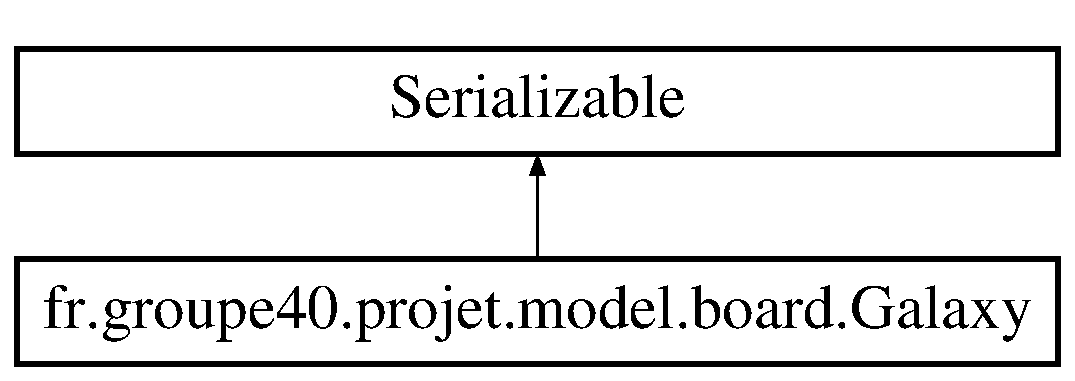
\includegraphics[height=2.000000cm]{classfr_1_1groupe40_1_1projet_1_1model_1_1board_1_1_galaxy}
\end{center}
\end{figure}
\subsection*{Public Member Functions}
\begin{DoxyCompactItemize}
\item 
\mbox{\Hypertarget{classfr_1_1groupe40_1_1projet_1_1model_1_1board_1_1_galaxy_acd002a00e4679b804002c05afb3b8308}\label{classfr_1_1groupe40_1_1projet_1_1model_1_1board_1_1_galaxy_acd002a00e4679b804002c05afb3b8308}} 
\hyperlink{classfr_1_1groupe40_1_1projet_1_1model_1_1board_1_1_galaxy_acd002a00e4679b804002c05afb3b8308}{Galaxy} ()
\begin{DoxyCompactList}\small\item\em Generate a game board with every parameters randomized. \end{DoxyCompactList}\item 
\hyperlink{classfr_1_1groupe40_1_1projet_1_1model_1_1board_1_1_galaxy_ae10e23d6a41a5b878123a8b03ec31e5a}{Galaxy} (\hyperlink{classfr_1_1groupe40_1_1projet_1_1model_1_1board_1_1_galaxy}{Galaxy} g)
\begin{DoxyCompactList}\small\item\em Generate a game board from another. \end{DoxyCompactList}\item 
\hyperlink{classfr_1_1groupe40_1_1projet_1_1model_1_1board_1_1_galaxy_ab214654e58ccf7bc40216d177cde0479}{Galaxy} (List$<$ \hyperlink{classfr_1_1groupe40_1_1projet_1_1model_1_1planets_1_1_planet}{Planet} $>$ planets, List$<$ \hyperlink{classfr_1_1groupe40_1_1projet_1_1model_1_1ships_1_1_squad}{Squad} $>$ squads)
\begin{DoxyCompactList}\small\item\em Generate a game board from an array of squads and planets. \end{DoxyCompactList}\item 
void \hyperlink{classfr_1_1groupe40_1_1projet_1_1model_1_1board_1_1_galaxy_ab3b17b740db263c25b80f7b9e6f33d24}{render} (Graphics\+Context gc)
\item 
\mbox{\Hypertarget{classfr_1_1groupe40_1_1projet_1_1model_1_1board_1_1_galaxy_a60fca62070a6cc902778ec3409a39c83}\label{classfr_1_1groupe40_1_1projet_1_1model_1_1board_1_1_galaxy_a60fca62070a6cc902778ec3409a39c83}} 
void \hyperlink{classfr_1_1groupe40_1_1projet_1_1model_1_1board_1_1_galaxy_a60fca62070a6cc902778ec3409a39c83}{update\+Squad\+Position} ()
\begin{DoxyCompactList}\small\item\em Main update function, manage AI, squads and has\+Lost. \end{DoxyCompactList}\item 
\mbox{\Hypertarget{classfr_1_1groupe40_1_1projet_1_1model_1_1board_1_1_galaxy_a32edba917f025f3ed2ff6d4723401dd1}\label{classfr_1_1groupe40_1_1projet_1_1model_1_1board_1_1_galaxy_a32edba917f025f3ed2ff6d4723401dd1}} 
void \hyperlink{classfr_1_1groupe40_1_1projet_1_1model_1_1board_1_1_galaxy_a32edba917f025f3ed2ff6d4723401dd1}{update\+AI} ()
\begin{DoxyCompactList}\small\item\em Manage the AI to send fleets. \end{DoxyCompactList}\item 
\mbox{\Hypertarget{classfr_1_1groupe40_1_1projet_1_1model_1_1board_1_1_galaxy_abad9a09b0c05e9092229a7406c8e1978}\label{classfr_1_1groupe40_1_1projet_1_1model_1_1board_1_1_galaxy_abad9a09b0c05e9092229a7406c8e1978}} 
void \hyperlink{classfr_1_1groupe40_1_1projet_1_1model_1_1board_1_1_galaxy_abad9a09b0c05e9092229a7406c8e1978}{update\+Garrison} ()
\begin{DoxyCompactList}\small\item\em update the garrison value of each planets \end{DoxyCompactList}\item 
\mbox{\Hypertarget{classfr_1_1groupe40_1_1projet_1_1model_1_1board_1_1_galaxy_afe5b556d02f5234c44ccfd505de5e2db}\label{classfr_1_1groupe40_1_1projet_1_1model_1_1board_1_1_galaxy_afe5b556d02f5234c44ccfd505de5e2db}} 
void \hyperlink{classfr_1_1groupe40_1_1projet_1_1model_1_1board_1_1_galaxy_afe5b556d02f5234c44ccfd505de5e2db}{update\+Waves\+Sending} ()
\begin{DoxyCompactList}\small\item\em send all a new wave if need for each squads \end{DoxyCompactList}\item 
boolean \hyperlink{classfr_1_1groupe40_1_1projet_1_1model_1_1board_1_1_galaxy_ad3ec27b73e7f093df14ca096395d10c2}{user\+Has\+Lost} (\hyperlink{classfr_1_1groupe40_1_1projet_1_1client_1_1_user}{User} u)
\begin{DoxyCompactList}\small\item\em Check if an user has lost. \end{DoxyCompactList}\item 
void \hyperlink{classfr_1_1groupe40_1_1projet_1_1model_1_1board_1_1_galaxy_a1cfe73fa7265d21c8c58162dd42acf58}{client\+Scroll\+Handler} (Direction direction)
\begin{DoxyCompactList}\small\item\em handle the scrolls event to change the percent of a fleet to send \end{DoxyCompactList}\item 
void \hyperlink{classfr_1_1groupe40_1_1projet_1_1model_1_1board_1_1_galaxy_a707f976a47503d6afab529da6a36a148}{collision\+Handler} (\hyperlink{classfr_1_1groupe40_1_1projet_1_1model_1_1ships_1_1_ship}{Ship} s, \hyperlink{classfr_1_1groupe40_1_1projet_1_1model_1_1planets_1_1_planet}{Planet} p)
\begin{DoxyCompactList}\small\item\em Manage the collisions between squads \& intermediate planets. \end{DoxyCompactList}\item 
boolean \hyperlink{classfr_1_1groupe40_1_1projet_1_1model_1_1board_1_1_galaxy_adb71c0d567ad5489d9f0d8890d604400}{is\+Collision} (\hyperlink{classfr_1_1groupe40_1_1projet_1_1model_1_1ships_1_1_ship}{Ship} s)
\begin{DoxyCompactList}\small\item\em check if there s a collision between a squad and every planet on board \end{DoxyCompactList}\item 
void \hyperlink{classfr_1_1groupe40_1_1projet_1_1model_1_1board_1_1_galaxy_aa24392147b91b61606b8e8e859ca3e23}{render\+Background} (Graphics\+Context gc)
\begin{DoxyCompactList}\small\item\em Render the background image. \end{DoxyCompactList}\item 
void \hyperlink{classfr_1_1groupe40_1_1projet_1_1model_1_1board_1_1_galaxy_a8490ed78537afb38bb28d86e4e37c312}{render\+Planets} (Graphics\+Context gc)
\begin{DoxyCompactList}\small\item\em Render each planets image. \end{DoxyCompactList}\item 
void \hyperlink{classfr_1_1groupe40_1_1projet_1_1model_1_1board_1_1_galaxy_a6fa32ff167eee765c18856e14679b281}{render\+Squads} (Graphics\+Context gc)
\begin{DoxyCompactList}\small\item\em Render every squads on board. \end{DoxyCompactList}\item 
void \hyperlink{classfr_1_1groupe40_1_1projet_1_1model_1_1board_1_1_galaxy_adbfc5609c012349d89f33849aa2787b0}{render\+Garrison} (Graphics\+Context gc)
\begin{DoxyCompactList}\small\item\em Render the garrison amount of each planets on board. \end{DoxyCompactList}\item 
void \hyperlink{classfr_1_1groupe40_1_1projet_1_1model_1_1board_1_1_galaxy_ab7d878b625cbb910e7eb20d0b3b3c260}{render\+Percentage\+Selected} (Graphics\+Context gc)
\begin{DoxyCompactList}\small\item\em Render the percentage of troups to send selected by the player. \end{DoxyCompactList}\item 
void \hyperlink{classfr_1_1groupe40_1_1projet_1_1model_1_1board_1_1_galaxy_aac749470d94e804f10e6891dbd043e03}{render\+Defeat} (Graphics\+Context gc)
\begin{DoxyCompactList}\small\item\em render in case of defeat //\+T\+O\+DO defeat rendering \end{DoxyCompactList}\item 
void \hyperlink{classfr_1_1groupe40_1_1projet_1_1model_1_1board_1_1_galaxy_aabdca1530440c8acec7f50c30af1a805}{render\+Explosion} (Graphics\+Context gc)
\begin{DoxyCompactList}\small\item\em render a explosion when a ship reach his destination \end{DoxyCompactList}\item 
void \hyperlink{classfr_1_1groupe40_1_1projet_1_1model_1_1board_1_1_galaxy_afcc91fd13d372426cae4eca41e115a11}{init\+Font} (Graphics\+Context gc)
\begin{DoxyCompactList}\small\item\em Init the default font style of the graphics context. \end{DoxyCompactList}\item 
Array\+List$<$ \hyperlink{classfr_1_1groupe40_1_1projet_1_1model_1_1ships_1_1_squad}{Squad} $>$ \hyperlink{classfr_1_1groupe40_1_1projet_1_1model_1_1board_1_1_galaxy_a76035e4de1484dfba7daf377127f80c0}{get\+Squads} ()
\begin{DoxyCompactList}\small\item\em Set the list containing every squads by another one. \end{DoxyCompactList}\item 
void \hyperlink{classfr_1_1groupe40_1_1projet_1_1model_1_1board_1_1_galaxy_a598d42d4b1e24f23d1e004a2e69c8959}{set\+Squads} (Array\+List$<$ \hyperlink{classfr_1_1groupe40_1_1projet_1_1model_1_1ships_1_1_squad}{Squad} $>$ squads)
\begin{DoxyCompactList}\small\item\em Return the list containing every squads on board. \end{DoxyCompactList}\item 
void \hyperlink{classfr_1_1groupe40_1_1projet_1_1model_1_1board_1_1_galaxy_a7f400bf11202afef051fccbc9cc727a9}{set\+Planets} (Array\+List$<$ \hyperlink{classfr_1_1groupe40_1_1projet_1_1model_1_1planets_1_1_planet}{Planet} $>$ planets)
\begin{DoxyCompactList}\small\item\em Set the list containing every planet by another one. \end{DoxyCompactList}\item 
Array\+List$<$ \hyperlink{classfr_1_1groupe40_1_1projet_1_1model_1_1planets_1_1_planet}{Planet} $>$ \hyperlink{classfr_1_1groupe40_1_1projet_1_1model_1_1board_1_1_galaxy_a9e97906db3f8da0d99dfcb0f272d476b}{get\+Planets} ()
\begin{DoxyCompactList}\small\item\em Return the list containing every planets on board. \end{DoxyCompactList}\item 
Image \hyperlink{classfr_1_1groupe40_1_1projet_1_1model_1_1board_1_1_galaxy_adc4718307d1288fe07acabd1f31415c9}{get\+Background} ()
\begin{DoxyCompactList}\small\item\em Return the background image. \end{DoxyCompactList}\item 
void \hyperlink{classfr_1_1groupe40_1_1projet_1_1model_1_1board_1_1_galaxy_a765e649c1488992dbf1247ae9a1adaf7}{set\+Background} (Image background)
\begin{DoxyCompactList}\small\item\em Set the background image. \end{DoxyCompactList}\end{DoxyCompactItemize}


\subsection{Detailed Description}
\textquotesingle{}Board\textquotesingle{} class. It contains the data of the game as ships, planets, ... 

\begin{DoxyAuthor}{Author}
Jordane Masson 

Sarah Portejoie 
\end{DoxyAuthor}


\subsection{Constructor \& Destructor Documentation}
\mbox{\Hypertarget{classfr_1_1groupe40_1_1projet_1_1model_1_1board_1_1_galaxy_ae10e23d6a41a5b878123a8b03ec31e5a}\label{classfr_1_1groupe40_1_1projet_1_1model_1_1board_1_1_galaxy_ae10e23d6a41a5b878123a8b03ec31e5a}} 
\index{fr\+::groupe40\+::projet\+::model\+::board\+::\+Galaxy@{fr\+::groupe40\+::projet\+::model\+::board\+::\+Galaxy}!Galaxy@{Galaxy}}
\index{Galaxy@{Galaxy}!fr\+::groupe40\+::projet\+::model\+::board\+::\+Galaxy@{fr\+::groupe40\+::projet\+::model\+::board\+::\+Galaxy}}
\subsubsection{\texorpdfstring{Galaxy()}{Galaxy()}\hspace{0.1cm}{\footnotesize\ttfamily [1/2]}}
{\footnotesize\ttfamily fr.\+groupe40.\+projet.\+model.\+board.\+Galaxy.\+Galaxy (\begin{DoxyParamCaption}\item[{\hyperlink{classfr_1_1groupe40_1_1projet_1_1model_1_1board_1_1_galaxy}{Galaxy}}]{g }\end{DoxyParamCaption})}



Generate a game board from another. 


\begin{DoxyParams}{Parameters}
{\em g} & The game board to copy from \\
\hline
\end{DoxyParams}
\mbox{\Hypertarget{classfr_1_1groupe40_1_1projet_1_1model_1_1board_1_1_galaxy_ab214654e58ccf7bc40216d177cde0479}\label{classfr_1_1groupe40_1_1projet_1_1model_1_1board_1_1_galaxy_ab214654e58ccf7bc40216d177cde0479}} 
\index{fr\+::groupe40\+::projet\+::model\+::board\+::\+Galaxy@{fr\+::groupe40\+::projet\+::model\+::board\+::\+Galaxy}!Galaxy@{Galaxy}}
\index{Galaxy@{Galaxy}!fr\+::groupe40\+::projet\+::model\+::board\+::\+Galaxy@{fr\+::groupe40\+::projet\+::model\+::board\+::\+Galaxy}}
\subsubsection{\texorpdfstring{Galaxy()}{Galaxy()}\hspace{0.1cm}{\footnotesize\ttfamily [2/2]}}
{\footnotesize\ttfamily fr.\+groupe40.\+projet.\+model.\+board.\+Galaxy.\+Galaxy (\begin{DoxyParamCaption}\item[{List$<$ \hyperlink{classfr_1_1groupe40_1_1projet_1_1model_1_1planets_1_1_planet}{Planet} $>$}]{planets,  }\item[{List$<$ \hyperlink{classfr_1_1groupe40_1_1projet_1_1model_1_1ships_1_1_squad}{Squad} $>$}]{squads }\end{DoxyParamCaption})}



Generate a game board from an array of squads and planets. 


\begin{DoxyParams}{Parameters}
{\em planets} & Planets that we want to have \\
\hline
{\em squads} & Squads already present \\
\hline
\end{DoxyParams}


\subsection{Member Function Documentation}
\mbox{\Hypertarget{classfr_1_1groupe40_1_1projet_1_1model_1_1board_1_1_galaxy_a1cfe73fa7265d21c8c58162dd42acf58}\label{classfr_1_1groupe40_1_1projet_1_1model_1_1board_1_1_galaxy_a1cfe73fa7265d21c8c58162dd42acf58}} 
\index{fr\+::groupe40\+::projet\+::model\+::board\+::\+Galaxy@{fr\+::groupe40\+::projet\+::model\+::board\+::\+Galaxy}!client\+Scroll\+Handler@{client\+Scroll\+Handler}}
\index{client\+Scroll\+Handler@{client\+Scroll\+Handler}!fr\+::groupe40\+::projet\+::model\+::board\+::\+Galaxy@{fr\+::groupe40\+::projet\+::model\+::board\+::\+Galaxy}}
\subsubsection{\texorpdfstring{client\+Scroll\+Handler()}{clientScrollHandler()}}
{\footnotesize\ttfamily void fr.\+groupe40.\+projet.\+model.\+board.\+Galaxy.\+client\+Scroll\+Handler (\begin{DoxyParamCaption}\item[{Direction}]{direction }\end{DoxyParamCaption})}



handle the scrolls event to change the percent of a fleet to send 


\begin{DoxyParams}{Parameters}
{\em action} & The scroll action (up or down case) \\
\hline
\end{DoxyParams}
\mbox{\Hypertarget{classfr_1_1groupe40_1_1projet_1_1model_1_1board_1_1_galaxy_a707f976a47503d6afab529da6a36a148}\label{classfr_1_1groupe40_1_1projet_1_1model_1_1board_1_1_galaxy_a707f976a47503d6afab529da6a36a148}} 
\index{fr\+::groupe40\+::projet\+::model\+::board\+::\+Galaxy@{fr\+::groupe40\+::projet\+::model\+::board\+::\+Galaxy}!collision\+Handler@{collision\+Handler}}
\index{collision\+Handler@{collision\+Handler}!fr\+::groupe40\+::projet\+::model\+::board\+::\+Galaxy@{fr\+::groupe40\+::projet\+::model\+::board\+::\+Galaxy}}
\subsubsection{\texorpdfstring{collision\+Handler()}{collisionHandler()}}
{\footnotesize\ttfamily void fr.\+groupe40.\+projet.\+model.\+board.\+Galaxy.\+collision\+Handler (\begin{DoxyParamCaption}\item[{\hyperlink{classfr_1_1groupe40_1_1projet_1_1model_1_1ships_1_1_ship}{Ship}}]{s,  }\item[{\hyperlink{classfr_1_1groupe40_1_1projet_1_1model_1_1planets_1_1_planet}{Planet}}]{p }\end{DoxyParamCaption})}



Manage the collisions between squads \& intermediate planets. 


\begin{DoxyParams}{Parameters}
{\em s} & The squad to manage \\
\hline
{\em p} & The planet to test collision with \\
\hline
\end{DoxyParams}
\mbox{\Hypertarget{classfr_1_1groupe40_1_1projet_1_1model_1_1board_1_1_galaxy_adc4718307d1288fe07acabd1f31415c9}\label{classfr_1_1groupe40_1_1projet_1_1model_1_1board_1_1_galaxy_adc4718307d1288fe07acabd1f31415c9}} 
\index{fr\+::groupe40\+::projet\+::model\+::board\+::\+Galaxy@{fr\+::groupe40\+::projet\+::model\+::board\+::\+Galaxy}!get\+Background@{get\+Background}}
\index{get\+Background@{get\+Background}!fr\+::groupe40\+::projet\+::model\+::board\+::\+Galaxy@{fr\+::groupe40\+::projet\+::model\+::board\+::\+Galaxy}}
\subsubsection{\texorpdfstring{get\+Background()}{getBackground()}}
{\footnotesize\ttfamily Image fr.\+groupe40.\+projet.\+model.\+board.\+Galaxy.\+get\+Background (\begin{DoxyParamCaption}{ }\end{DoxyParamCaption})}



Return the background image. 

\begin{DoxyReturn}{Returns}
Image 
\end{DoxyReturn}
\mbox{\Hypertarget{classfr_1_1groupe40_1_1projet_1_1model_1_1board_1_1_galaxy_a9e97906db3f8da0d99dfcb0f272d476b}\label{classfr_1_1groupe40_1_1projet_1_1model_1_1board_1_1_galaxy_a9e97906db3f8da0d99dfcb0f272d476b}} 
\index{fr\+::groupe40\+::projet\+::model\+::board\+::\+Galaxy@{fr\+::groupe40\+::projet\+::model\+::board\+::\+Galaxy}!get\+Planets@{get\+Planets}}
\index{get\+Planets@{get\+Planets}!fr\+::groupe40\+::projet\+::model\+::board\+::\+Galaxy@{fr\+::groupe40\+::projet\+::model\+::board\+::\+Galaxy}}
\subsubsection{\texorpdfstring{get\+Planets()}{getPlanets()}}
{\footnotesize\ttfamily Array\+List$<$\hyperlink{classfr_1_1groupe40_1_1projet_1_1model_1_1planets_1_1_planet}{Planet}$>$ fr.\+groupe40.\+projet.\+model.\+board.\+Galaxy.\+get\+Planets (\begin{DoxyParamCaption}{ }\end{DoxyParamCaption})}



Return the list containing every planets on board. 

\begin{DoxyReturn}{Returns}

\end{DoxyReturn}
\mbox{\Hypertarget{classfr_1_1groupe40_1_1projet_1_1model_1_1board_1_1_galaxy_a76035e4de1484dfba7daf377127f80c0}\label{classfr_1_1groupe40_1_1projet_1_1model_1_1board_1_1_galaxy_a76035e4de1484dfba7daf377127f80c0}} 
\index{fr\+::groupe40\+::projet\+::model\+::board\+::\+Galaxy@{fr\+::groupe40\+::projet\+::model\+::board\+::\+Galaxy}!get\+Squads@{get\+Squads}}
\index{get\+Squads@{get\+Squads}!fr\+::groupe40\+::projet\+::model\+::board\+::\+Galaxy@{fr\+::groupe40\+::projet\+::model\+::board\+::\+Galaxy}}
\subsubsection{\texorpdfstring{get\+Squads()}{getSquads()}}
{\footnotesize\ttfamily Array\+List$<$\hyperlink{classfr_1_1groupe40_1_1projet_1_1model_1_1ships_1_1_squad}{Squad}$>$ fr.\+groupe40.\+projet.\+model.\+board.\+Galaxy.\+get\+Squads (\begin{DoxyParamCaption}{ }\end{DoxyParamCaption})}



Set the list containing every squads by another one. 


\begin{DoxyParams}{Parameters}
{\em planets} & \\
\hline
\end{DoxyParams}
\mbox{\Hypertarget{classfr_1_1groupe40_1_1projet_1_1model_1_1board_1_1_galaxy_afcc91fd13d372426cae4eca41e115a11}\label{classfr_1_1groupe40_1_1projet_1_1model_1_1board_1_1_galaxy_afcc91fd13d372426cae4eca41e115a11}} 
\index{fr\+::groupe40\+::projet\+::model\+::board\+::\+Galaxy@{fr\+::groupe40\+::projet\+::model\+::board\+::\+Galaxy}!init\+Font@{init\+Font}}
\index{init\+Font@{init\+Font}!fr\+::groupe40\+::projet\+::model\+::board\+::\+Galaxy@{fr\+::groupe40\+::projet\+::model\+::board\+::\+Galaxy}}
\subsubsection{\texorpdfstring{init\+Font()}{initFont()}}
{\footnotesize\ttfamily void fr.\+groupe40.\+projet.\+model.\+board.\+Galaxy.\+init\+Font (\begin{DoxyParamCaption}\item[{Graphics\+Context}]{gc }\end{DoxyParamCaption})}



Init the default font style of the graphics context. 


\begin{DoxyParams}{Parameters}
{\em gc} & \\
\hline
\end{DoxyParams}
\mbox{\Hypertarget{classfr_1_1groupe40_1_1projet_1_1model_1_1board_1_1_galaxy_adb71c0d567ad5489d9f0d8890d604400}\label{classfr_1_1groupe40_1_1projet_1_1model_1_1board_1_1_galaxy_adb71c0d567ad5489d9f0d8890d604400}} 
\index{fr\+::groupe40\+::projet\+::model\+::board\+::\+Galaxy@{fr\+::groupe40\+::projet\+::model\+::board\+::\+Galaxy}!is\+Collision@{is\+Collision}}
\index{is\+Collision@{is\+Collision}!fr\+::groupe40\+::projet\+::model\+::board\+::\+Galaxy@{fr\+::groupe40\+::projet\+::model\+::board\+::\+Galaxy}}
\subsubsection{\texorpdfstring{is\+Collision()}{isCollision()}}
{\footnotesize\ttfamily boolean fr.\+groupe40.\+projet.\+model.\+board.\+Galaxy.\+is\+Collision (\begin{DoxyParamCaption}\item[{\hyperlink{classfr_1_1groupe40_1_1projet_1_1model_1_1ships_1_1_ship}{Ship}}]{s }\end{DoxyParamCaption})}



check if there s a collision between a squad and every planet on board 


\begin{DoxyParams}{Parameters}
{\em s} & the squad to check \\
\hline
\end{DoxyParams}
\begin{DoxyReturn}{Returns}
true if there s a collision, else false 
\end{DoxyReturn}
\mbox{\Hypertarget{classfr_1_1groupe40_1_1projet_1_1model_1_1board_1_1_galaxy_ab3b17b740db263c25b80f7b9e6f33d24}\label{classfr_1_1groupe40_1_1projet_1_1model_1_1board_1_1_galaxy_ab3b17b740db263c25b80f7b9e6f33d24}} 
\index{fr\+::groupe40\+::projet\+::model\+::board\+::\+Galaxy@{fr\+::groupe40\+::projet\+::model\+::board\+::\+Galaxy}!render@{render}}
\index{render@{render}!fr\+::groupe40\+::projet\+::model\+::board\+::\+Galaxy@{fr\+::groupe40\+::projet\+::model\+::board\+::\+Galaxy}}
\subsubsection{\texorpdfstring{render()}{render()}}
{\footnotesize\ttfamily void fr.\+groupe40.\+projet.\+model.\+board.\+Galaxy.\+render (\begin{DoxyParamCaption}\item[{Graphics\+Context}]{gc }\end{DoxyParamCaption})}

rendering function 
\begin{DoxyParams}{Parameters}
{\em gc} & \\
\hline
\end{DoxyParams}
\mbox{\Hypertarget{classfr_1_1groupe40_1_1projet_1_1model_1_1board_1_1_galaxy_aa24392147b91b61606b8e8e859ca3e23}\label{classfr_1_1groupe40_1_1projet_1_1model_1_1board_1_1_galaxy_aa24392147b91b61606b8e8e859ca3e23}} 
\index{fr\+::groupe40\+::projet\+::model\+::board\+::\+Galaxy@{fr\+::groupe40\+::projet\+::model\+::board\+::\+Galaxy}!render\+Background@{render\+Background}}
\index{render\+Background@{render\+Background}!fr\+::groupe40\+::projet\+::model\+::board\+::\+Galaxy@{fr\+::groupe40\+::projet\+::model\+::board\+::\+Galaxy}}
\subsubsection{\texorpdfstring{render\+Background()}{renderBackground()}}
{\footnotesize\ttfamily void fr.\+groupe40.\+projet.\+model.\+board.\+Galaxy.\+render\+Background (\begin{DoxyParamCaption}\item[{Graphics\+Context}]{gc }\end{DoxyParamCaption})}



Render the background image. 


\begin{DoxyParams}{Parameters}
{\em gc} & \\
\hline
\end{DoxyParams}
\mbox{\Hypertarget{classfr_1_1groupe40_1_1projet_1_1model_1_1board_1_1_galaxy_aac749470d94e804f10e6891dbd043e03}\label{classfr_1_1groupe40_1_1projet_1_1model_1_1board_1_1_galaxy_aac749470d94e804f10e6891dbd043e03}} 
\index{fr\+::groupe40\+::projet\+::model\+::board\+::\+Galaxy@{fr\+::groupe40\+::projet\+::model\+::board\+::\+Galaxy}!render\+Defeat@{render\+Defeat}}
\index{render\+Defeat@{render\+Defeat}!fr\+::groupe40\+::projet\+::model\+::board\+::\+Galaxy@{fr\+::groupe40\+::projet\+::model\+::board\+::\+Galaxy}}
\subsubsection{\texorpdfstring{render\+Defeat()}{renderDefeat()}}
{\footnotesize\ttfamily void fr.\+groupe40.\+projet.\+model.\+board.\+Galaxy.\+render\+Defeat (\begin{DoxyParamCaption}\item[{Graphics\+Context}]{gc }\end{DoxyParamCaption})}



render in case of defeat //\+T\+O\+DO defeat rendering 


\begin{DoxyParams}{Parameters}
{\em gc} & the Graphics Context \\
\hline
\end{DoxyParams}
\mbox{\Hypertarget{classfr_1_1groupe40_1_1projet_1_1model_1_1board_1_1_galaxy_aabdca1530440c8acec7f50c30af1a805}\label{classfr_1_1groupe40_1_1projet_1_1model_1_1board_1_1_galaxy_aabdca1530440c8acec7f50c30af1a805}} 
\index{fr\+::groupe40\+::projet\+::model\+::board\+::\+Galaxy@{fr\+::groupe40\+::projet\+::model\+::board\+::\+Galaxy}!render\+Explosion@{render\+Explosion}}
\index{render\+Explosion@{render\+Explosion}!fr\+::groupe40\+::projet\+::model\+::board\+::\+Galaxy@{fr\+::groupe40\+::projet\+::model\+::board\+::\+Galaxy}}
\subsubsection{\texorpdfstring{render\+Explosion()}{renderExplosion()}}
{\footnotesize\ttfamily void fr.\+groupe40.\+projet.\+model.\+board.\+Galaxy.\+render\+Explosion (\begin{DoxyParamCaption}\item[{Graphics\+Context}]{gc }\end{DoxyParamCaption})}



render a explosion when a ship reach his destination 


\begin{DoxyParams}{Parameters}
{\em gc} & \\
\hline
\end{DoxyParams}
\mbox{\Hypertarget{classfr_1_1groupe40_1_1projet_1_1model_1_1board_1_1_galaxy_adbfc5609c012349d89f33849aa2787b0}\label{classfr_1_1groupe40_1_1projet_1_1model_1_1board_1_1_galaxy_adbfc5609c012349d89f33849aa2787b0}} 
\index{fr\+::groupe40\+::projet\+::model\+::board\+::\+Galaxy@{fr\+::groupe40\+::projet\+::model\+::board\+::\+Galaxy}!render\+Garrison@{render\+Garrison}}
\index{render\+Garrison@{render\+Garrison}!fr\+::groupe40\+::projet\+::model\+::board\+::\+Galaxy@{fr\+::groupe40\+::projet\+::model\+::board\+::\+Galaxy}}
\subsubsection{\texorpdfstring{render\+Garrison()}{renderGarrison()}}
{\footnotesize\ttfamily void fr.\+groupe40.\+projet.\+model.\+board.\+Galaxy.\+render\+Garrison (\begin{DoxyParamCaption}\item[{Graphics\+Context}]{gc }\end{DoxyParamCaption})}



Render the garrison amount of each planets on board. 


\begin{DoxyParams}{Parameters}
{\em gc} & \\
\hline
\end{DoxyParams}
\mbox{\Hypertarget{classfr_1_1groupe40_1_1projet_1_1model_1_1board_1_1_galaxy_ab7d878b625cbb910e7eb20d0b3b3c260}\label{classfr_1_1groupe40_1_1projet_1_1model_1_1board_1_1_galaxy_ab7d878b625cbb910e7eb20d0b3b3c260}} 
\index{fr\+::groupe40\+::projet\+::model\+::board\+::\+Galaxy@{fr\+::groupe40\+::projet\+::model\+::board\+::\+Galaxy}!render\+Percentage\+Selected@{render\+Percentage\+Selected}}
\index{render\+Percentage\+Selected@{render\+Percentage\+Selected}!fr\+::groupe40\+::projet\+::model\+::board\+::\+Galaxy@{fr\+::groupe40\+::projet\+::model\+::board\+::\+Galaxy}}
\subsubsection{\texorpdfstring{render\+Percentage\+Selected()}{renderPercentageSelected()}}
{\footnotesize\ttfamily void fr.\+groupe40.\+projet.\+model.\+board.\+Galaxy.\+render\+Percentage\+Selected (\begin{DoxyParamCaption}\item[{Graphics\+Context}]{gc }\end{DoxyParamCaption})}



Render the percentage of troups to send selected by the player. 


\begin{DoxyParams}{Parameters}
{\em gc} & \\
\hline
\end{DoxyParams}
\mbox{\Hypertarget{classfr_1_1groupe40_1_1projet_1_1model_1_1board_1_1_galaxy_a8490ed78537afb38bb28d86e4e37c312}\label{classfr_1_1groupe40_1_1projet_1_1model_1_1board_1_1_galaxy_a8490ed78537afb38bb28d86e4e37c312}} 
\index{fr\+::groupe40\+::projet\+::model\+::board\+::\+Galaxy@{fr\+::groupe40\+::projet\+::model\+::board\+::\+Galaxy}!render\+Planets@{render\+Planets}}
\index{render\+Planets@{render\+Planets}!fr\+::groupe40\+::projet\+::model\+::board\+::\+Galaxy@{fr\+::groupe40\+::projet\+::model\+::board\+::\+Galaxy}}
\subsubsection{\texorpdfstring{render\+Planets()}{renderPlanets()}}
{\footnotesize\ttfamily void fr.\+groupe40.\+projet.\+model.\+board.\+Galaxy.\+render\+Planets (\begin{DoxyParamCaption}\item[{Graphics\+Context}]{gc }\end{DoxyParamCaption})}



Render each planets image. 


\begin{DoxyParams}{Parameters}
{\em gc} & \\
\hline
\end{DoxyParams}
\mbox{\Hypertarget{classfr_1_1groupe40_1_1projet_1_1model_1_1board_1_1_galaxy_a6fa32ff167eee765c18856e14679b281}\label{classfr_1_1groupe40_1_1projet_1_1model_1_1board_1_1_galaxy_a6fa32ff167eee765c18856e14679b281}} 
\index{fr\+::groupe40\+::projet\+::model\+::board\+::\+Galaxy@{fr\+::groupe40\+::projet\+::model\+::board\+::\+Galaxy}!render\+Squads@{render\+Squads}}
\index{render\+Squads@{render\+Squads}!fr\+::groupe40\+::projet\+::model\+::board\+::\+Galaxy@{fr\+::groupe40\+::projet\+::model\+::board\+::\+Galaxy}}
\subsubsection{\texorpdfstring{render\+Squads()}{renderSquads()}}
{\footnotesize\ttfamily void fr.\+groupe40.\+projet.\+model.\+board.\+Galaxy.\+render\+Squads (\begin{DoxyParamCaption}\item[{Graphics\+Context}]{gc }\end{DoxyParamCaption})}



Render every squads on board. 


\begin{DoxyParams}{Parameters}
{\em gc} & \\
\hline
\end{DoxyParams}
\mbox{\Hypertarget{classfr_1_1groupe40_1_1projet_1_1model_1_1board_1_1_galaxy_a765e649c1488992dbf1247ae9a1adaf7}\label{classfr_1_1groupe40_1_1projet_1_1model_1_1board_1_1_galaxy_a765e649c1488992dbf1247ae9a1adaf7}} 
\index{fr\+::groupe40\+::projet\+::model\+::board\+::\+Galaxy@{fr\+::groupe40\+::projet\+::model\+::board\+::\+Galaxy}!set\+Background@{set\+Background}}
\index{set\+Background@{set\+Background}!fr\+::groupe40\+::projet\+::model\+::board\+::\+Galaxy@{fr\+::groupe40\+::projet\+::model\+::board\+::\+Galaxy}}
\subsubsection{\texorpdfstring{set\+Background()}{setBackground()}}
{\footnotesize\ttfamily void fr.\+groupe40.\+projet.\+model.\+board.\+Galaxy.\+set\+Background (\begin{DoxyParamCaption}\item[{Image}]{background }\end{DoxyParamCaption})}



Set the background image. 


\begin{DoxyParams}{Parameters}
{\em background} & \\
\hline
\end{DoxyParams}
\mbox{\Hypertarget{classfr_1_1groupe40_1_1projet_1_1model_1_1board_1_1_galaxy_a7f400bf11202afef051fccbc9cc727a9}\label{classfr_1_1groupe40_1_1projet_1_1model_1_1board_1_1_galaxy_a7f400bf11202afef051fccbc9cc727a9}} 
\index{fr\+::groupe40\+::projet\+::model\+::board\+::\+Galaxy@{fr\+::groupe40\+::projet\+::model\+::board\+::\+Galaxy}!set\+Planets@{set\+Planets}}
\index{set\+Planets@{set\+Planets}!fr\+::groupe40\+::projet\+::model\+::board\+::\+Galaxy@{fr\+::groupe40\+::projet\+::model\+::board\+::\+Galaxy}}
\subsubsection{\texorpdfstring{set\+Planets()}{setPlanets()}}
{\footnotesize\ttfamily void fr.\+groupe40.\+projet.\+model.\+board.\+Galaxy.\+set\+Planets (\begin{DoxyParamCaption}\item[{Array\+List$<$ \hyperlink{classfr_1_1groupe40_1_1projet_1_1model_1_1planets_1_1_planet}{Planet} $>$}]{planets }\end{DoxyParamCaption})}



Set the list containing every planet by another one. 


\begin{DoxyParams}{Parameters}
{\em planets} & \\
\hline
\end{DoxyParams}
\mbox{\Hypertarget{classfr_1_1groupe40_1_1projet_1_1model_1_1board_1_1_galaxy_a598d42d4b1e24f23d1e004a2e69c8959}\label{classfr_1_1groupe40_1_1projet_1_1model_1_1board_1_1_galaxy_a598d42d4b1e24f23d1e004a2e69c8959}} 
\index{fr\+::groupe40\+::projet\+::model\+::board\+::\+Galaxy@{fr\+::groupe40\+::projet\+::model\+::board\+::\+Galaxy}!set\+Squads@{set\+Squads}}
\index{set\+Squads@{set\+Squads}!fr\+::groupe40\+::projet\+::model\+::board\+::\+Galaxy@{fr\+::groupe40\+::projet\+::model\+::board\+::\+Galaxy}}
\subsubsection{\texorpdfstring{set\+Squads()}{setSquads()}}
{\footnotesize\ttfamily void fr.\+groupe40.\+projet.\+model.\+board.\+Galaxy.\+set\+Squads (\begin{DoxyParamCaption}\item[{Array\+List$<$ \hyperlink{classfr_1_1groupe40_1_1projet_1_1model_1_1ships_1_1_squad}{Squad} $>$}]{squads }\end{DoxyParamCaption})}



Return the list containing every squads on board. 

\begin{DoxyReturn}{Returns}

\end{DoxyReturn}
\mbox{\Hypertarget{classfr_1_1groupe40_1_1projet_1_1model_1_1board_1_1_galaxy_ad3ec27b73e7f093df14ca096395d10c2}\label{classfr_1_1groupe40_1_1projet_1_1model_1_1board_1_1_galaxy_ad3ec27b73e7f093df14ca096395d10c2}} 
\index{fr\+::groupe40\+::projet\+::model\+::board\+::\+Galaxy@{fr\+::groupe40\+::projet\+::model\+::board\+::\+Galaxy}!user\+Has\+Lost@{user\+Has\+Lost}}
\index{user\+Has\+Lost@{user\+Has\+Lost}!fr\+::groupe40\+::projet\+::model\+::board\+::\+Galaxy@{fr\+::groupe40\+::projet\+::model\+::board\+::\+Galaxy}}
\subsubsection{\texorpdfstring{user\+Has\+Lost()}{userHasLost()}}
{\footnotesize\ttfamily boolean fr.\+groupe40.\+projet.\+model.\+board.\+Galaxy.\+user\+Has\+Lost (\begin{DoxyParamCaption}\item[{\hyperlink{classfr_1_1groupe40_1_1projet_1_1client_1_1_user}{User}}]{u }\end{DoxyParamCaption})}



Check if an user has lost. 


\begin{DoxyParams}{Parameters}
{\em u} & the user to check \\
\hline
\end{DoxyParams}
\begin{DoxyReturn}{Returns}
true if he has last, else false 
\end{DoxyReturn}


The documentation for this class was generated from the following file\+:\begin{DoxyCompactItemize}
\item 
src/fr/groupe40/projet/model/board/Galaxy.\+java\end{DoxyCompactItemize}

\hypertarget{classfr_1_1groupe40_1_1projet_1_1model_1_1board_1_1_galaxy_generator}{}\section{fr.\+groupe40.\+projet.\+model.\+board.\+Galaxy\+Generator Class Reference}
\label{classfr_1_1groupe40_1_1projet_1_1model_1_1board_1_1_galaxy_generator}\index{fr.\+groupe40.\+projet.\+model.\+board.\+Galaxy\+Generator@{fr.\+groupe40.\+projet.\+model.\+board.\+Galaxy\+Generator}}
\subsection*{Public Member Functions}
\begin{DoxyCompactItemize}
\item 
\mbox{\Hypertarget{classfr_1_1groupe40_1_1projet_1_1model_1_1board_1_1_galaxy_generator_a7af2998c5098fa02bf6dfd0c794dfe2d}\label{classfr_1_1groupe40_1_1projet_1_1model_1_1board_1_1_galaxy_generator_a7af2998c5098fa02bf6dfd0c794dfe2d}} 
void \mbox{\hyperlink{classfr_1_1groupe40_1_1projet_1_1model_1_1board_1_1_galaxy_generator_a7af2998c5098fa02bf6dfd0c794dfe2d}{generate\+Planets}} ()
\begin{DoxyCompactList}\small\item\em Generate the planets for the galaxy initialization. \end{DoxyCompactList}\item 
Array\+List$<$ \mbox{\hyperlink{classfr_1_1groupe40_1_1projet_1_1model_1_1planets_1_1_planet}{Planet}} $>$ \mbox{\hyperlink{classfr_1_1groupe40_1_1projet_1_1model_1_1board_1_1_galaxy_generator_a025a232f305b1465f38a73fac918dbb5}{get\+Planets}} ()
\item 
void \mbox{\hyperlink{classfr_1_1groupe40_1_1projet_1_1model_1_1board_1_1_galaxy_generator_a67bac9f8bd2561972535ec64c63340ce}{set\+Planets}} (Array\+List$<$ \mbox{\hyperlink{classfr_1_1groupe40_1_1projet_1_1model_1_1planets_1_1_planet}{Planet}} $>$ planets)
\end{DoxyCompactItemize}


\subsection{Member Function Documentation}
\mbox{\Hypertarget{classfr_1_1groupe40_1_1projet_1_1model_1_1board_1_1_galaxy_generator_a025a232f305b1465f38a73fac918dbb5}\label{classfr_1_1groupe40_1_1projet_1_1model_1_1board_1_1_galaxy_generator_a025a232f305b1465f38a73fac918dbb5}} 
\index{fr\+::groupe40\+::projet\+::model\+::board\+::\+Galaxy\+Generator@{fr\+::groupe40\+::projet\+::model\+::board\+::\+Galaxy\+Generator}!get\+Planets@{get\+Planets}}
\index{get\+Planets@{get\+Planets}!fr\+::groupe40\+::projet\+::model\+::board\+::\+Galaxy\+Generator@{fr\+::groupe40\+::projet\+::model\+::board\+::\+Galaxy\+Generator}}
\subsubsection{\texorpdfstring{get\+Planets()}{getPlanets()}}
{\footnotesize\ttfamily Array\+List$<$\mbox{\hyperlink{classfr_1_1groupe40_1_1projet_1_1model_1_1planets_1_1_planet}{Planet}}$>$ fr.\+groupe40.\+projet.\+model.\+board.\+Galaxy\+Generator.\+get\+Planets (\begin{DoxyParamCaption}{ }\end{DoxyParamCaption})}

\begin{DoxyReturn}{Returns}
the planets 
\end{DoxyReturn}
\mbox{\Hypertarget{classfr_1_1groupe40_1_1projet_1_1model_1_1board_1_1_galaxy_generator_a67bac9f8bd2561972535ec64c63340ce}\label{classfr_1_1groupe40_1_1projet_1_1model_1_1board_1_1_galaxy_generator_a67bac9f8bd2561972535ec64c63340ce}} 
\index{fr\+::groupe40\+::projet\+::model\+::board\+::\+Galaxy\+Generator@{fr\+::groupe40\+::projet\+::model\+::board\+::\+Galaxy\+Generator}!set\+Planets@{set\+Planets}}
\index{set\+Planets@{set\+Planets}!fr\+::groupe40\+::projet\+::model\+::board\+::\+Galaxy\+Generator@{fr\+::groupe40\+::projet\+::model\+::board\+::\+Galaxy\+Generator}}
\subsubsection{\texorpdfstring{set\+Planets()}{setPlanets()}}
{\footnotesize\ttfamily void fr.\+groupe40.\+projet.\+model.\+board.\+Galaxy\+Generator.\+set\+Planets (\begin{DoxyParamCaption}\item[{Array\+List$<$ \mbox{\hyperlink{classfr_1_1groupe40_1_1projet_1_1model_1_1planets_1_1_planet}{Planet}} $>$}]{planets }\end{DoxyParamCaption})}


\begin{DoxyParams}{Parameters}
{\em planets} & the planets to set \\
\hline
\end{DoxyParams}


The documentation for this class was generated from the following file\+:\begin{DoxyCompactItemize}
\item 
src/fr/groupe40/projet/model/board/Galaxy\+Generator.\+java\end{DoxyCompactItemize}

\hypertarget{classfr_1_1groupe40_1_1projet_1_1_game}{}\section{fr.\+groupe40.\+projet.\+Game Class Reference}
\label{classfr_1_1groupe40_1_1projet_1_1_game}\index{fr.\+groupe40.\+projet.\+Game@{fr.\+groupe40.\+projet.\+Game}}
Inheritance diagram for fr.\+groupe40.\+projet.\+Game\+:\begin{figure}[H]
\begin{center}
\leavevmode
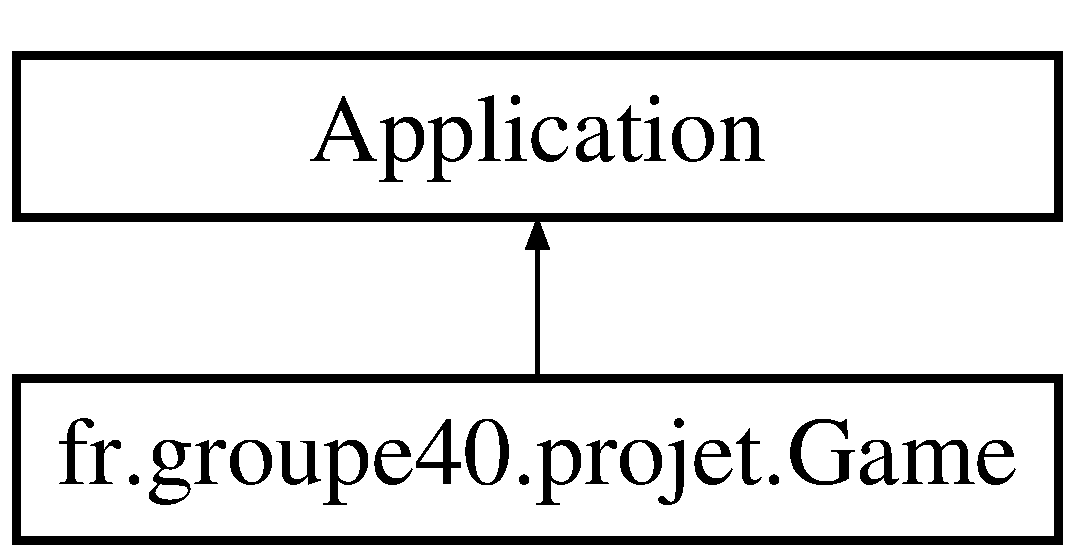
\includegraphics[height=2.000000cm]{classfr_1_1groupe40_1_1projet_1_1_game}
\end{center}
\end{figure}
\subsection*{Public Member Functions}
\begin{DoxyCompactItemize}
\item 
void \mbox{\hyperlink{classfr_1_1groupe40_1_1projet_1_1_game_a3700e488ecfb4fe5ff34bda5cb82b414}{start}} (Stage stage)
\end{DoxyCompactItemize}
\subsection*{Static Public Member Functions}
\begin{DoxyCompactItemize}
\item 
\mbox{\Hypertarget{classfr_1_1groupe40_1_1projet_1_1_game_a690e2c3a3122844e099ac0dd3c2f60d7}\label{classfr_1_1groupe40_1_1projet_1_1_game_a690e2c3a3122844e099ac0dd3c2f60d7}} 
static void {\bfseries main} (String\mbox{[}$\,$\mbox{]} args)
\end{DoxyCompactItemize}


\subsection{Member Function Documentation}
\mbox{\Hypertarget{classfr_1_1groupe40_1_1projet_1_1_game_a3700e488ecfb4fe5ff34bda5cb82b414}\label{classfr_1_1groupe40_1_1projet_1_1_game_a3700e488ecfb4fe5ff34bda5cb82b414}} 
\index{fr\+::groupe40\+::projet\+::\+Game@{fr\+::groupe40\+::projet\+::\+Game}!start@{start}}
\index{start@{start}!fr\+::groupe40\+::projet\+::\+Game@{fr\+::groupe40\+::projet\+::\+Game}}
\subsubsection{\texorpdfstring{start()}{start()}}
{\footnotesize\ttfamily void fr.\+groupe40.\+projet.\+Game.\+start (\begin{DoxyParamCaption}\item[{Stage}]{stage }\end{DoxyParamCaption})}

Window and game kernel creation ~\newline
~\newline
 Saver ~\newline
 Rendering 

The documentation for this class was generated from the following file\+:\begin{DoxyCompactItemize}
\item 
src/fr/groupe40/projet/Game.\+java\end{DoxyCompactItemize}

\hypertarget{classfr_1_1groupe40_1_1projet_1_1client_1_1handler_1_1_interaction_handler}{}\section{fr.\+groupe40.\+projet.\+client.\+handler.\+Interaction\+Handler Class Reference}
\label{classfr_1_1groupe40_1_1projet_1_1client_1_1handler_1_1_interaction_handler}\index{fr.\+groupe40.\+projet.\+client.\+handler.\+Interaction\+Handler@{fr.\+groupe40.\+projet.\+client.\+handler.\+Interaction\+Handler}}
Inheritance diagram for fr.\+groupe40.\+projet.\+client.\+handler.\+Interaction\+Handler\+:\begin{figure}[H]
\begin{center}
\leavevmode
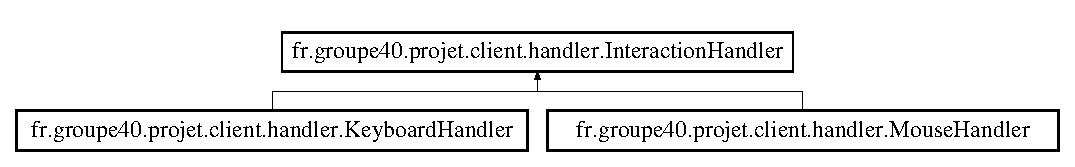
\includegraphics[height=1.794872cm]{classfr_1_1groupe40_1_1projet_1_1client_1_1handler_1_1_interaction_handler}
\end{center}
\end{figure}
\subsection*{Public Member Functions}
\begin{DoxyCompactItemize}
\item 
\mbox{\Hypertarget{classfr_1_1groupe40_1_1projet_1_1client_1_1handler_1_1_interaction_handler_a8dd863e883515616cc850b0bfdf739d6}\label{classfr_1_1groupe40_1_1projet_1_1client_1_1handler_1_1_interaction_handler_a8dd863e883515616cc850b0bfdf739d6}} 
{\bfseries Interaction\+Handler} (\hyperlink{classfr_1_1groupe40_1_1projet_1_1model_1_1board_1_1_galaxy}{Galaxy} galaxy)
\item 
\mbox{\Hypertarget{classfr_1_1groupe40_1_1projet_1_1client_1_1handler_1_1_interaction_handler_a5c28d18fd9bcfa863f40fcace497f9f3}\label{classfr_1_1groupe40_1_1projet_1_1client_1_1handler_1_1_interaction_handler_a5c28d18fd9bcfa863f40fcace497f9f3}} 
Event\+Handler$<$ Mouse\+Event $>$ {\bfseries get\+Mouse\+Pressed\+Event} ()
\item 
\mbox{\Hypertarget{classfr_1_1groupe40_1_1projet_1_1client_1_1handler_1_1_interaction_handler_ac57c4caa8e5e43adbc4e4eec4985bb1e}\label{classfr_1_1groupe40_1_1projet_1_1client_1_1handler_1_1_interaction_handler_ac57c4caa8e5e43adbc4e4eec4985bb1e}} 
void {\bfseries set\+Mouse\+Pressed\+Event} (Event\+Handler$<$ Mouse\+Event $>$ mouse\+Pressed\+Event)
\item 
\mbox{\Hypertarget{classfr_1_1groupe40_1_1projet_1_1client_1_1handler_1_1_interaction_handler_a06995a2ecf5e028168a3f6609b6f7474}\label{classfr_1_1groupe40_1_1projet_1_1client_1_1handler_1_1_interaction_handler_a06995a2ecf5e028168a3f6609b6f7474}} 
Event\+Handler$<$ Mouse\+Event $>$ {\bfseries get\+Mouse\+Dragged\+Event} ()
\item 
\mbox{\Hypertarget{classfr_1_1groupe40_1_1projet_1_1client_1_1handler_1_1_interaction_handler_ab79eaad9e04d563e63eda350e8a29fb2}\label{classfr_1_1groupe40_1_1projet_1_1client_1_1handler_1_1_interaction_handler_ab79eaad9e04d563e63eda350e8a29fb2}} 
void {\bfseries set\+Mouse\+Dragged\+Event} (Event\+Handler$<$ Mouse\+Event $>$ mouse\+Dragged\+Event)
\item 
\mbox{\Hypertarget{classfr_1_1groupe40_1_1projet_1_1client_1_1handler_1_1_interaction_handler_a2ded2c50060e147f219c8d0d1a371018}\label{classfr_1_1groupe40_1_1projet_1_1client_1_1handler_1_1_interaction_handler_a2ded2c50060e147f219c8d0d1a371018}} 
Event\+Handler$<$ Scroll\+Event $>$ {\bfseries get\+Scroll\+Event} ()
\item 
\mbox{\Hypertarget{classfr_1_1groupe40_1_1projet_1_1client_1_1handler_1_1_interaction_handler_a2f82e0247f4e7282c58435f778fd90cc}\label{classfr_1_1groupe40_1_1projet_1_1client_1_1handler_1_1_interaction_handler_a2f82e0247f4e7282c58435f778fd90cc}} 
void {\bfseries set\+Scroll\+Event} (Event\+Handler$<$ Scroll\+Event $>$ scroll\+Event)
\item 
\mbox{\Hypertarget{classfr_1_1groupe40_1_1projet_1_1client_1_1handler_1_1_interaction_handler_a1998207353f48dbf08bdbd58c301fb57}\label{classfr_1_1groupe40_1_1projet_1_1client_1_1handler_1_1_interaction_handler_a1998207353f48dbf08bdbd58c301fb57}} 
\hyperlink{classfr_1_1groupe40_1_1projet_1_1model_1_1board_1_1_galaxy}{Galaxy} {\bfseries get\+Galaxy} ()
\item 
\mbox{\Hypertarget{classfr_1_1groupe40_1_1projet_1_1client_1_1handler_1_1_interaction_handler_a0b8b96a543adcd6eba599d445891885d}\label{classfr_1_1groupe40_1_1projet_1_1client_1_1handler_1_1_interaction_handler_a0b8b96a543adcd6eba599d445891885d}} 
void {\bfseries set\+Galaxy} (\hyperlink{classfr_1_1groupe40_1_1projet_1_1model_1_1board_1_1_galaxy}{Galaxy} galaxy)
\end{DoxyCompactItemize}
\subsection*{Protected Attributes}
\begin{DoxyCompactItemize}
\item 
\mbox{\Hypertarget{classfr_1_1groupe40_1_1projet_1_1client_1_1handler_1_1_interaction_handler_a39d69fa50a2af5e3403d5ba85e08d354}\label{classfr_1_1groupe40_1_1projet_1_1client_1_1handler_1_1_interaction_handler_a39d69fa50a2af5e3403d5ba85e08d354}} 
\hyperlink{classfr_1_1groupe40_1_1projet_1_1model_1_1board_1_1_galaxy}{Galaxy} {\bfseries galaxy}
\end{DoxyCompactItemize}


The documentation for this class was generated from the following file\+:\begin{DoxyCompactItemize}
\item 
src/fr/groupe40/projet/client/handler/Interaction\+Handler.\+java\end{DoxyCompactItemize}

\hypertarget{classfr_1_1groupe40_1_1projet_1_1client_1_1handler_1_1_keyboard_handler}{}\section{fr.\+groupe40.\+projet.\+client.\+handler.\+Keyboard\+Handler Class Reference}
\label{classfr_1_1groupe40_1_1projet_1_1client_1_1handler_1_1_keyboard_handler}\index{fr.\+groupe40.\+projet.\+client.\+handler.\+Keyboard\+Handler@{fr.\+groupe40.\+projet.\+client.\+handler.\+Keyboard\+Handler}}


The documentation for this class was generated from the following file\+:\begin{DoxyCompactItemize}
\item 
src/fr/groupe40/projet/client/handler/Keyboard\+Handler.\+java\end{DoxyCompactItemize}

\hypertarget{classfr_1_1groupe40_1_1projet_1_1window_1_1_loading_screen}{}\section{fr.\+groupe40.\+projet.\+window.\+Loading\+Screen Class Reference}
\label{classfr_1_1groupe40_1_1projet_1_1window_1_1_loading_screen}\index{fr.\+groupe40.\+projet.\+window.\+Loading\+Screen@{fr.\+groupe40.\+projet.\+window.\+Loading\+Screen}}


The documentation for this class was generated from the following file\+:\begin{DoxyCompactItemize}
\item 
src/fr/groupe40/projet/window/Loading\+Screen.\+java\end{DoxyCompactItemize}

\hypertarget{classfr_1_1groupe40_1_1projet_1_1window_1_1_main_menu}{}\section{fr.\+groupe40.\+projet.\+window.\+Main\+Menu Class Reference}
\label{classfr_1_1groupe40_1_1projet_1_1window_1_1_main_menu}\index{fr.\+groupe40.\+projet.\+window.\+Main\+Menu@{fr.\+groupe40.\+projet.\+window.\+Main\+Menu}}


The documentation for this class was generated from the following file\+:\begin{DoxyCompactItemize}
\item 
src/fr/groupe40/projet/window/Main\+Menu.\+java\end{DoxyCompactItemize}

\hypertarget{classfr_1_1groupe40_1_1projet_1_1client_1_1handler_1_1_mouse_handler}{}\section{fr.\+groupe40.\+projet.\+client.\+handler.\+Mouse\+Handler Class Reference}
\label{classfr_1_1groupe40_1_1projet_1_1client_1_1handler_1_1_mouse_handler}\index{fr.\+groupe40.\+projet.\+client.\+handler.\+Mouse\+Handler@{fr.\+groupe40.\+projet.\+client.\+handler.\+Mouse\+Handler}}


The documentation for this class was generated from the following file\+:\begin{DoxyCompactItemize}
\item 
src/fr/groupe40/projet/client/handler/Mouse\+Handler.\+java\end{DoxyCompactItemize}

\hypertarget{classfr_1_1groupe40_1_1projet_1_1events_1_1_pirate_assault}{}\section{fr.\+groupe40.\+projet.\+events.\+Pirate\+Assault Class Reference}
\label{classfr_1_1groupe40_1_1projet_1_1events_1_1_pirate_assault}\index{fr.\+groupe40.\+projet.\+events.\+Pirate\+Assault@{fr.\+groupe40.\+projet.\+events.\+Pirate\+Assault}}


The documentation for this class was generated from the following file\+:\begin{DoxyCompactItemize}
\item 
src/fr/groupe40/projet/events/Pirate\+Assault.\+java\end{DoxyCompactItemize}

\hypertarget{classfr_1_1groupe40_1_1projet_1_1model_1_1planets_1_1_planet}{}\section{fr.\+groupe40.\+projet.\+model.\+planets.\+Planet Class Reference}
\label{classfr_1_1groupe40_1_1projet_1_1model_1_1planets_1_1_planet}\index{fr.\+groupe40.\+projet.\+model.\+planets.\+Planet@{fr.\+groupe40.\+projet.\+model.\+planets.\+Planet}}


Abstract class of the general type \char`\"{}planet\char`\"{}.  


Inheritance diagram for fr.\+groupe40.\+projet.\+model.\+planets.\+Planet\+:\begin{figure}[H]
\begin{center}
\leavevmode
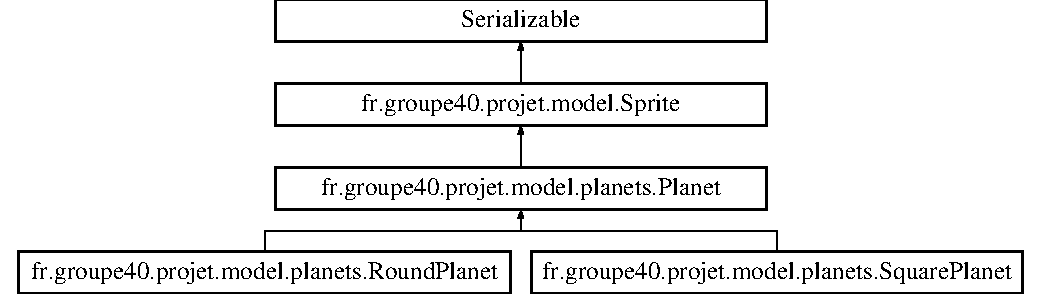
\includegraphics[height=3.957597cm]{classfr_1_1groupe40_1_1projet_1_1model_1_1planets_1_1_planet}
\end{center}
\end{figure}
\subsection*{Public Member Functions}
\begin{DoxyCompactItemize}
\item 
\hyperlink{classfr_1_1groupe40_1_1projet_1_1model_1_1planets_1_1_planet_a7cdf092f3e8443176362cf97ddcd11ae}{Planet} (String path, \hyperlink{classfr_1_1groupe40_1_1projet_1_1client_1_1_user}{User} ruler, int x, int y)
\begin{DoxyCompactList}\small\item\em Constructor of a planet. \end{DoxyCompactList}\item 
boolean \hyperlink{classfr_1_1groupe40_1_1projet_1_1model_1_1planets_1_1_planet_a14c09ad18bf0c963662ee45d0c6f07a1}{is\+Inside\+Planet} (double x, double y)
\begin{DoxyCompactList}\small\item\em check if a position is in a planet \end{DoxyCompactList}\item 
\mbox{\Hypertarget{classfr_1_1groupe40_1_1projet_1_1model_1_1planets_1_1_planet_a6db5bb259c3c2889b0285b0472fc6a76}\label{classfr_1_1groupe40_1_1projet_1_1model_1_1planets_1_1_planet_a6db5bb259c3c2889b0285b0472fc6a76}} 
void \hyperlink{classfr_1_1groupe40_1_1projet_1_1model_1_1planets_1_1_planet_a6db5bb259c3c2889b0285b0472fc6a76}{update\+Garrison} ()
\begin{DoxyCompactList}\small\item\em update the garrison value of this planet if not neutral \end{DoxyCompactList}\item 
int \hyperlink{classfr_1_1groupe40_1_1projet_1_1model_1_1planets_1_1_planet_a745df6537c22855fc854381c7ad2c029}{calculate\+Next\+Position} ()
\begin{DoxyCompactList}\small\item\em find his place in the universe \end{DoxyCompactList}\item 
int \hyperlink{classfr_1_1groupe40_1_1projet_1_1model_1_1planets_1_1_planet_a55af7887127afab452dec09d5d149d90}{update\+Planete\+Position} ()
\begin{DoxyCompactList}\small\item\em check new position for generation \end{DoxyCompactList}\item 
\mbox{\Hypertarget{classfr_1_1groupe40_1_1projet_1_1model_1_1planets_1_1_planet_af412d3420465e77b44fb404c1f2b2b09}\label{classfr_1_1groupe40_1_1projet_1_1model_1_1planets_1_1_planet_af412d3420465e77b44fb404c1f2b2b09}} 
String {\bfseries to\+String} ()
\item 
\mbox{\Hypertarget{classfr_1_1groupe40_1_1projet_1_1model_1_1planets_1_1_planet_aefe3771eb229fe25e8d09605057f6d00}\label{classfr_1_1groupe40_1_1projet_1_1model_1_1planets_1_1_planet_aefe3771eb229fe25e8d09605057f6d00}} 
int {\bfseries get\+Produce\+\_\+rate} ()
\item 
\mbox{\Hypertarget{classfr_1_1groupe40_1_1projet_1_1model_1_1planets_1_1_planet_ab725243f7aa413631c9dc428dee571de}\label{classfr_1_1groupe40_1_1projet_1_1model_1_1planets_1_1_planet_ab725243f7aa413631c9dc428dee571de}} 
void {\bfseries set\+Produce\+\_\+rate} (int produce\+\_\+rate)
\item 
\mbox{\Hypertarget{classfr_1_1groupe40_1_1projet_1_1model_1_1planets_1_1_planet_a3e88a9159386f7fd54ce7ef51144505b}\label{classfr_1_1groupe40_1_1projet_1_1model_1_1planets_1_1_planet_a3e88a9159386f7fd54ce7ef51144505b}} 
int {\bfseries get\+Troups} ()
\item 
\mbox{\Hypertarget{classfr_1_1groupe40_1_1projet_1_1model_1_1planets_1_1_planet_a4ca3243d99385baed5462d4478ee5e9b}\label{classfr_1_1groupe40_1_1projet_1_1model_1_1planets_1_1_planet_a4ca3243d99385baed5462d4478ee5e9b}} 
void {\bfseries set\+Troups} (int troups)
\item 
\mbox{\Hypertarget{classfr_1_1groupe40_1_1projet_1_1model_1_1planets_1_1_planet_a80f0d147f16e2ef34f3ee3addf05dabe}\label{classfr_1_1groupe40_1_1projet_1_1model_1_1planets_1_1_planet_a80f0d147f16e2ef34f3ee3addf05dabe}} 
\hyperlink{classfr_1_1groupe40_1_1projet_1_1model_1_1ships_1_1_ship_type}{Ship\+Type} {\bfseries get\+Ships\+\_\+type} ()
\item 
\mbox{\Hypertarget{classfr_1_1groupe40_1_1projet_1_1model_1_1planets_1_1_planet_a78187d3031a81c7cbd281b9aa6eac0bc}\label{classfr_1_1groupe40_1_1projet_1_1model_1_1planets_1_1_planet_a78187d3031a81c7cbd281b9aa6eac0bc}} 
void {\bfseries set\+Ships\+\_\+type} (\hyperlink{classfr_1_1groupe40_1_1projet_1_1model_1_1ships_1_1_ship_type}{Ship\+Type} ships\+\_\+type)
\item 
\mbox{\Hypertarget{classfr_1_1groupe40_1_1projet_1_1model_1_1planets_1_1_planet_a17d6b5e960300fe739ecb1e40f7a76b2}\label{classfr_1_1groupe40_1_1projet_1_1model_1_1planets_1_1_planet_a17d6b5e960300fe739ecb1e40f7a76b2}} 
boolean {\bfseries is\+Selected} ()
\item 
\mbox{\Hypertarget{classfr_1_1groupe40_1_1projet_1_1model_1_1planets_1_1_planet_ae3f4907ff4759f62887b055aaaa1c12e}\label{classfr_1_1groupe40_1_1projet_1_1model_1_1planets_1_1_planet_ae3f4907ff4759f62887b055aaaa1c12e}} 
void {\bfseries set\+Selected} (boolean selected)
\end{DoxyCompactItemize}


\subsection{Detailed Description}
Abstract class of the general type \char`\"{}planet\char`\"{}. 

\begin{DoxyAuthor}{Author}
Jordane Masson 

Sarah Portejoie 
\end{DoxyAuthor}


\subsection{Constructor \& Destructor Documentation}
\mbox{\Hypertarget{classfr_1_1groupe40_1_1projet_1_1model_1_1planets_1_1_planet_a7cdf092f3e8443176362cf97ddcd11ae}\label{classfr_1_1groupe40_1_1projet_1_1model_1_1planets_1_1_planet_a7cdf092f3e8443176362cf97ddcd11ae}} 
\index{fr\+::groupe40\+::projet\+::model\+::planets\+::\+Planet@{fr\+::groupe40\+::projet\+::model\+::planets\+::\+Planet}!Planet@{Planet}}
\index{Planet@{Planet}!fr\+::groupe40\+::projet\+::model\+::planets\+::\+Planet@{fr\+::groupe40\+::projet\+::model\+::planets\+::\+Planet}}
\subsubsection{\texorpdfstring{Planet()}{Planet()}}
{\footnotesize\ttfamily fr.\+groupe40.\+projet.\+model.\+planets.\+Planet.\+Planet (\begin{DoxyParamCaption}\item[{String}]{path,  }\item[{\hyperlink{classfr_1_1groupe40_1_1projet_1_1client_1_1_user}{User}}]{ruler,  }\item[{int}]{x,  }\item[{int}]{y }\end{DoxyParamCaption})}



Constructor of a planet. 


\begin{DoxyParams}{Parameters}
{\em path} & the string image path \\
\hline
{\em ruler} & the beginning ruler of this planet \\
\hline
{\em x} & top left x position \\
\hline
{\em y} & top left y position \\
\hline
\end{DoxyParams}


\subsection{Member Function Documentation}
\mbox{\Hypertarget{classfr_1_1groupe40_1_1projet_1_1model_1_1planets_1_1_planet_a745df6537c22855fc854381c7ad2c029}\label{classfr_1_1groupe40_1_1projet_1_1model_1_1planets_1_1_planet_a745df6537c22855fc854381c7ad2c029}} 
\index{fr\+::groupe40\+::projet\+::model\+::planets\+::\+Planet@{fr\+::groupe40\+::projet\+::model\+::planets\+::\+Planet}!calculate\+Next\+Position@{calculate\+Next\+Position}}
\index{calculate\+Next\+Position@{calculate\+Next\+Position}!fr\+::groupe40\+::projet\+::model\+::planets\+::\+Planet@{fr\+::groupe40\+::projet\+::model\+::planets\+::\+Planet}}
\subsubsection{\texorpdfstring{calculate\+Next\+Position()}{calculateNextPosition()}}
{\footnotesize\ttfamily int fr.\+groupe40.\+projet.\+model.\+planets.\+Planet.\+calculate\+Next\+Position (\begin{DoxyParamCaption}{ }\end{DoxyParamCaption})}



find his place in the universe 

\begin{DoxyReturn}{Returns}
0 if his position is correct, else error value 
\end{DoxyReturn}
\mbox{\Hypertarget{classfr_1_1groupe40_1_1projet_1_1model_1_1planets_1_1_planet_a14c09ad18bf0c963662ee45d0c6f07a1}\label{classfr_1_1groupe40_1_1projet_1_1model_1_1planets_1_1_planet_a14c09ad18bf0c963662ee45d0c6f07a1}} 
\index{fr\+::groupe40\+::projet\+::model\+::planets\+::\+Planet@{fr\+::groupe40\+::projet\+::model\+::planets\+::\+Planet}!is\+Inside\+Planet@{is\+Inside\+Planet}}
\index{is\+Inside\+Planet@{is\+Inside\+Planet}!fr\+::groupe40\+::projet\+::model\+::planets\+::\+Planet@{fr\+::groupe40\+::projet\+::model\+::planets\+::\+Planet}}
\subsubsection{\texorpdfstring{is\+Inside\+Planet()}{isInsidePlanet()}}
{\footnotesize\ttfamily boolean fr.\+groupe40.\+projet.\+model.\+planets.\+Planet.\+is\+Inside\+Planet (\begin{DoxyParamCaption}\item[{double}]{x,  }\item[{double}]{y }\end{DoxyParamCaption})}



check if a position is in a planet 


\begin{DoxyParams}{Parameters}
{\em x} & \\
\hline
{\em y} & \\
\hline
\end{DoxyParams}
\begin{DoxyReturn}{Returns}
true if inside, else false 
\end{DoxyReturn}
\mbox{\Hypertarget{classfr_1_1groupe40_1_1projet_1_1model_1_1planets_1_1_planet_a55af7887127afab452dec09d5d149d90}\label{classfr_1_1groupe40_1_1projet_1_1model_1_1planets_1_1_planet_a55af7887127afab452dec09d5d149d90}} 
\index{fr\+::groupe40\+::projet\+::model\+::planets\+::\+Planet@{fr\+::groupe40\+::projet\+::model\+::planets\+::\+Planet}!update\+Planete\+Position@{update\+Planete\+Position}}
\index{update\+Planete\+Position@{update\+Planete\+Position}!fr\+::groupe40\+::projet\+::model\+::planets\+::\+Planet@{fr\+::groupe40\+::projet\+::model\+::planets\+::\+Planet}}
\subsubsection{\texorpdfstring{update\+Planete\+Position()}{updatePlanetePosition()}}
{\footnotesize\ttfamily int fr.\+groupe40.\+projet.\+model.\+planets.\+Planet.\+update\+Planete\+Position (\begin{DoxyParamCaption}{ }\end{DoxyParamCaption})}



check new position for generation 

\begin{DoxyReturn}{Returns}
0 if ok. -\/1 if unable to generate 
\end{DoxyReturn}


The documentation for this class was generated from the following file\+:\begin{DoxyCompactItemize}
\item 
src/fr/groupe40/projet/model/planets/Planet.\+java\end{DoxyCompactItemize}

\hypertarget{classfr_1_1groupe40_1_1projet_1_1model_1_1planets_1_1_round_planet}{}\section{fr.\+groupe40.\+projet.\+model.\+planets.\+Round\+Planet Class Reference}
\label{classfr_1_1groupe40_1_1projet_1_1model_1_1planets_1_1_round_planet}\index{fr.\+groupe40.\+projet.\+model.\+planets.\+Round\+Planet@{fr.\+groupe40.\+projet.\+model.\+planets.\+Round\+Planet}}
Inheritance diagram for fr.\+groupe40.\+projet.\+model.\+planets.\+Round\+Planet\+:\begin{figure}[H]
\begin{center}
\leavevmode
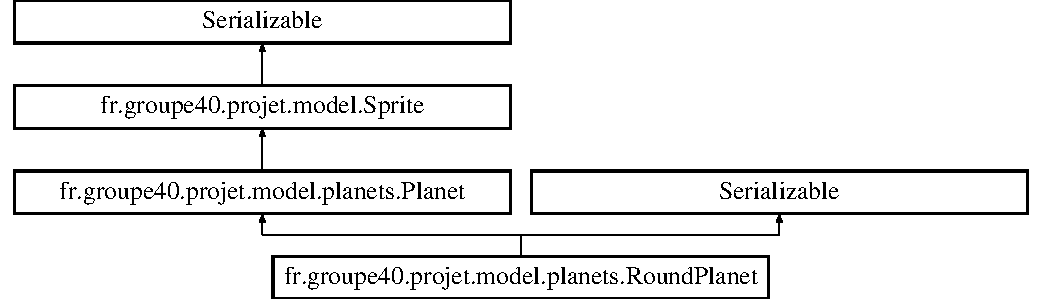
\includegraphics[height=4.000000cm]{classfr_1_1groupe40_1_1projet_1_1model_1_1planets_1_1_round_planet}
\end{center}
\end{figure}
\subsection*{Public Member Functions}
\begin{DoxyCompactItemize}
\item 
\mbox{\Hypertarget{classfr_1_1groupe40_1_1projet_1_1model_1_1planets_1_1_round_planet_a48bb1db2b253cfc635bf1c3a8a55df13}\label{classfr_1_1groupe40_1_1projet_1_1model_1_1planets_1_1_round_planet_a48bb1db2b253cfc635bf1c3a8a55df13}} 
{\bfseries Round\+Planet} (\mbox{\hyperlink{classfr_1_1groupe40_1_1projet_1_1client_1_1_user}{User}} ruler, boolean is\+Planet, int x, int y)
\end{DoxyCompactItemize}


The documentation for this class was generated from the following file\+:\begin{DoxyCompactItemize}
\item 
src/fr/groupe40/projet/model/planets/Round\+Planet.\+java\end{DoxyCompactItemize}

\hypertarget{classfr_1_1groupe40_1_1projet_1_1window_1_1_settings_menu}{}\section{fr.\+groupe40.\+projet.\+window.\+Settings\+Menu Class Reference}
\label{classfr_1_1groupe40_1_1projet_1_1window_1_1_settings_menu}\index{fr.\+groupe40.\+projet.\+window.\+Settings\+Menu@{fr.\+groupe40.\+projet.\+window.\+Settings\+Menu}}


The documentation for this class was generated from the following file\+:\begin{DoxyCompactItemize}
\item 
src/fr/groupe40/projet/window/Settings\+Menu.\+java\end{DoxyCompactItemize}

\hypertarget{classfr_1_1groupe40_1_1projet_1_1model_1_1ships_1_1_ship}{}\section{fr.\+groupe40.\+projet.\+model.\+ships.\+Ship Class Reference}
\label{classfr_1_1groupe40_1_1projet_1_1model_1_1ships_1_1_ship}\index{fr.\+groupe40.\+projet.\+model.\+ships.\+Ship@{fr.\+groupe40.\+projet.\+model.\+ships.\+Ship}}


\hyperlink{classfr_1_1groupe40_1_1projet_1_1model_1_1ships_1_1_ship}{Ship} of a squad, contains the destination, src, ...  


Inheritance diagram for fr.\+groupe40.\+projet.\+model.\+ships.\+Ship\+:\begin{figure}[H]
\begin{center}
\leavevmode
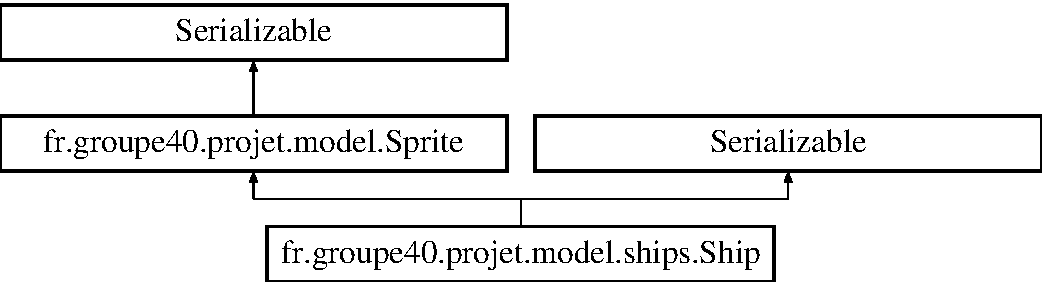
\includegraphics[height=3.000000cm]{classfr_1_1groupe40_1_1projet_1_1model_1_1ships_1_1_ship}
\end{center}
\end{figure}
\subsection*{Public Member Functions}
\begin{DoxyCompactItemize}
\item 
\hyperlink{classfr_1_1groupe40_1_1projet_1_1model_1_1ships_1_1_ship_a50b240c8ac54e3944b63208c5df4cb91}{Ship} (String path, \hyperlink{classfr_1_1groupe40_1_1projet_1_1client_1_1_user}{User} ruler, \hyperlink{classfr_1_1groupe40_1_1projet_1_1model_1_1planets_1_1_planet}{Planet} \hyperlink{classfr_1_1groupe40_1_1projet_1_1model_1_1ships_1_1_ship_a19eb504f8a0c0e263aff1e85e5e7557a}{destination}, \hyperlink{classfr_1_1groupe40_1_1projet_1_1model_1_1planets_1_1_planet}{Planet} source, double x\+\_\+init, double y\+\_\+init, \hyperlink{classfr_1_1groupe40_1_1projet_1_1model_1_1ships_1_1_ship_type}{Ship\+Type} ship\+\_\+type)
\begin{DoxyCompactList}\small\item\em constructor of the ship object \end{DoxyCompactList}\item 
\mbox{\Hypertarget{classfr_1_1groupe40_1_1projet_1_1model_1_1ships_1_1_ship_a4526f55c2d198ce47e0f64b924ec6b43}\label{classfr_1_1groupe40_1_1projet_1_1model_1_1ships_1_1_ship_a4526f55c2d198ce47e0f64b924ec6b43}} 
boolean \hyperlink{classfr_1_1groupe40_1_1projet_1_1model_1_1ships_1_1_ship_a4526f55c2d198ce47e0f64b924ec6b43}{reached\+\_\+destination} ()
\begin{DoxyCompactList}\small\item\em Check if the ship has reached his destination, and handle this case. \end{DoxyCompactList}\item 
void \hyperlink{classfr_1_1groupe40_1_1projet_1_1model_1_1ships_1_1_ship_adfd10eb0bb2fe81b8612a9da7acc8148}{calc\+\_\+next\+\_\+position} (List$<$ \hyperlink{classfr_1_1groupe40_1_1projet_1_1model_1_1planets_1_1_planet}{Planet} $>$ planets)
\begin{DoxyCompactList}\small\item\em Calculate the next position and provides collision handler. \end{DoxyCompactList}\item 
\hyperlink{enumfr_1_1groupe40_1_1projet_1_1util_1_1constants_1_1_collision}{Collision} \hyperlink{classfr_1_1groupe40_1_1projet_1_1model_1_1ships_1_1_ship_af8015208641d46aa77545db2cc71c149}{whereis\+\_\+collision} (double x, double y, double speed, List$<$ \hyperlink{classfr_1_1groupe40_1_1projet_1_1model_1_1planets_1_1_planet}{Planet} $>$ planets)
\begin{DoxyCompactList}\small\item\em return where is the collision between a ship and every planets of a list \end{DoxyCompactList}\item 
void \hyperlink{classfr_1_1groupe40_1_1projet_1_1model_1_1ships_1_1_ship_aab898b49dfc4d08d3b8ac7b08d936697}{top\+\_\+collision\+\_\+mover} (double x, double y, double centre\+\_\+x, double centre\+\_\+y, double speed)
\begin{DoxyCompactList}\small\item\em Next position calculation when there s a collision in the upper side. \end{DoxyCompactList}\item 
void \hyperlink{classfr_1_1groupe40_1_1projet_1_1model_1_1ships_1_1_ship_a88644a9fdb0c146f6f9ba556326e7122}{bottom\+\_\+collision\+\_\+mover} (double x, double y, double centre\+\_\+x, double centre\+\_\+y, double speed)
\begin{DoxyCompactList}\small\item\em Next position calculation when there s a collision in the bottom side. \end{DoxyCompactList}\item 
void \hyperlink{classfr_1_1groupe40_1_1projet_1_1model_1_1ships_1_1_ship_a2908d837a3d3515380ce728f42b43b52}{left\+\_\+collision\+\_\+mover} (double x, double y, double centre\+\_\+x, double centre\+\_\+y, double speed)
\begin{DoxyCompactList}\small\item\em Next position calculation when there s a collision in the left side. \end{DoxyCompactList}\item 
void \hyperlink{classfr_1_1groupe40_1_1projet_1_1model_1_1ships_1_1_ship_a1e045760991d3d6594a41348128f6bef}{right\+\_\+collision\+\_\+mover} (double x, double y, double centre\+\_\+x, double centre\+\_\+y, double speed)
\begin{DoxyCompactList}\small\item\em Next position calculation when there s a collision in the right side. \end{DoxyCompactList}\item 
double \hyperlink{classfr_1_1groupe40_1_1projet_1_1model_1_1ships_1_1_ship_aba9445d4839238bdb88b4e99229fdd89}{destination\+\_\+angle} ()
\begin{DoxyCompactList}\small\item\em calculate the angle between a ship and his destination \end{DoxyCompactList}\item 
void \hyperlink{classfr_1_1groupe40_1_1projet_1_1model_1_1ships_1_1_ship_af506b10fa38eae488d02c08fccb3d7df}{no\+\_\+collision\+\_\+mover} (double x, double y, double centre\+\_\+x, double centre\+\_\+y, double speed)
\begin{DoxyCompactList}\small\item\em case when there s no collision for a ship \end{DoxyCompactList}\item 
void \hyperlink{classfr_1_1groupe40_1_1projet_1_1model_1_1ships_1_1_ship_af4fcf4bf2b5fdad442d33491c69b2019}{update\+\_\+position} (List$<$ \hyperlink{classfr_1_1groupe40_1_1projet_1_1model_1_1planets_1_1_planet}{Planet} $>$ planets)
\begin{DoxyCompactList}\small\item\em Update the position of this ship. \end{DoxyCompactList}\item 
\mbox{\Hypertarget{classfr_1_1groupe40_1_1projet_1_1model_1_1ships_1_1_ship_a2d132d6ec4b6025f82cf687916bb7f95}\label{classfr_1_1groupe40_1_1projet_1_1model_1_1ships_1_1_ship_a2d132d6ec4b6025f82cf687916bb7f95}} 
void \hyperlink{classfr_1_1groupe40_1_1projet_1_1model_1_1ships_1_1_ship_a2d132d6ec4b6025f82cf687916bb7f95}{remove} ()
\begin{DoxyCompactList}\small\item\em prepare his removal from the squad list \end{DoxyCompactList}\item 
\hyperlink{classfr_1_1groupe40_1_1projet_1_1model_1_1ships_1_1_ship_type}{Ship\+Type} \hyperlink{classfr_1_1groupe40_1_1projet_1_1model_1_1ships_1_1_ship_af2ee5ad92b1137894f467076e158fc95}{get\+Ship\+\_\+type} ()
\item 
void \hyperlink{classfr_1_1groupe40_1_1projet_1_1model_1_1ships_1_1_ship_a7bbf63c47f60e88943422e04877c161f}{set\+Ship\+\_\+type} (\hyperlink{classfr_1_1groupe40_1_1projet_1_1model_1_1ships_1_1_ship_type}{Ship\+Type} ship\+\_\+type)
\item 
\hyperlink{classfr_1_1groupe40_1_1projet_1_1model_1_1planets_1_1_planet}{Planet} \hyperlink{classfr_1_1groupe40_1_1projet_1_1model_1_1ships_1_1_ship_ac4f24f0b83dfec2b15cf455c79b75e24}{get\+Destination} ()
\item 
void \hyperlink{classfr_1_1groupe40_1_1projet_1_1model_1_1ships_1_1_ship_abdc025f4461e7efd9a2ee6af93d9bef3}{set\+Destination} (\hyperlink{classfr_1_1groupe40_1_1projet_1_1model_1_1planets_1_1_planet}{Planet} \hyperlink{classfr_1_1groupe40_1_1projet_1_1model_1_1ships_1_1_ship_a19eb504f8a0c0e263aff1e85e5e7557a}{destination})
\item 
\hyperlink{classfr_1_1groupe40_1_1projet_1_1model_1_1planets_1_1_planet}{Planet} \hyperlink{classfr_1_1groupe40_1_1projet_1_1model_1_1ships_1_1_ship_a0bad8c1701c7a6bee319ae8671228d6f}{get\+Source} ()
\item 
void \hyperlink{classfr_1_1groupe40_1_1projet_1_1model_1_1ships_1_1_ship_aa48b0a9238306da4fcc27a37dfc50829}{set\+Source} (\hyperlink{classfr_1_1groupe40_1_1projet_1_1model_1_1planets_1_1_planet}{Planet} source)
\item 
boolean \hyperlink{classfr_1_1groupe40_1_1projet_1_1model_1_1ships_1_1_ship_a81d13eda5cf767c710e6d82407172d47}{is\+Reached} ()
\item 
void \hyperlink{classfr_1_1groupe40_1_1projet_1_1model_1_1ships_1_1_ship_a5a3e2ba94e01cce27b168365e53e0cde}{set\+Reached} (boolean \hyperlink{classfr_1_1groupe40_1_1projet_1_1model_1_1ships_1_1_ship_abd5ae4da4bce134894098a111d7378c3}{reached})
\item 
\hyperlink{classfr_1_1groupe40_1_1projet_1_1model_1_1planets_1_1_planet}{Planet} \hyperlink{classfr_1_1groupe40_1_1projet_1_1model_1_1ships_1_1_ship_a7fb131bafd7937973eecd26870796dd8}{get\+Collision} ()
\item 
void \hyperlink{classfr_1_1groupe40_1_1projet_1_1model_1_1ships_1_1_ship_aad6f47714d9aa1e212ce9ee5e1a8d22a}{set\+Collision} (\hyperlink{classfr_1_1groupe40_1_1projet_1_1model_1_1planets_1_1_planet}{Planet} collision)
\item 
double \hyperlink{classfr_1_1groupe40_1_1projet_1_1model_1_1ships_1_1_ship_aae0aceeef0cac73a3c384324e9d8b867}{get\+Speed} ()
\end{DoxyCompactItemize}
\subsection*{Protected Attributes}
\begin{DoxyCompactItemize}
\item 
\mbox{\Hypertarget{classfr_1_1groupe40_1_1projet_1_1model_1_1ships_1_1_ship_a19eb504f8a0c0e263aff1e85e5e7557a}\label{classfr_1_1groupe40_1_1projet_1_1model_1_1ships_1_1_ship_a19eb504f8a0c0e263aff1e85e5e7557a}} 
\hyperlink{classfr_1_1groupe40_1_1projet_1_1model_1_1planets_1_1_planet}{Planet} \hyperlink{classfr_1_1groupe40_1_1projet_1_1model_1_1ships_1_1_ship_a19eb504f8a0c0e263aff1e85e5e7557a}{destination}
\begin{DoxyCompactList}\small\item\em Source and Destination planets. \end{DoxyCompactList}\item 
\mbox{\Hypertarget{classfr_1_1groupe40_1_1projet_1_1model_1_1ships_1_1_ship_abd5ae4da4bce134894098a111d7378c3}\label{classfr_1_1groupe40_1_1projet_1_1model_1_1ships_1_1_ship_abd5ae4da4bce134894098a111d7378c3}} 
boolean \hyperlink{classfr_1_1groupe40_1_1projet_1_1model_1_1ships_1_1_ship_abd5ae4da4bce134894098a111d7378c3}{reached}
\begin{DoxyCompactList}\small\item\em If this ships has reacher or not his destination. \end{DoxyCompactList}\end{DoxyCompactItemize}


\subsection{Detailed Description}
\hyperlink{classfr_1_1groupe40_1_1projet_1_1model_1_1ships_1_1_ship}{Ship} of a squad, contains the destination, src, ... 

\begin{DoxyAuthor}{Author}
Jordane Masson 

Sarah Portejoie 
\end{DoxyAuthor}


\subsection{Constructor \& Destructor Documentation}
\mbox{\Hypertarget{classfr_1_1groupe40_1_1projet_1_1model_1_1ships_1_1_ship_a50b240c8ac54e3944b63208c5df4cb91}\label{classfr_1_1groupe40_1_1projet_1_1model_1_1ships_1_1_ship_a50b240c8ac54e3944b63208c5df4cb91}} 
\index{fr\+::groupe40\+::projet\+::model\+::ships\+::\+Ship@{fr\+::groupe40\+::projet\+::model\+::ships\+::\+Ship}!Ship@{Ship}}
\index{Ship@{Ship}!fr\+::groupe40\+::projet\+::model\+::ships\+::\+Ship@{fr\+::groupe40\+::projet\+::model\+::ships\+::\+Ship}}
\subsubsection{\texorpdfstring{Ship()}{Ship()}}
{\footnotesize\ttfamily fr.\+groupe40.\+projet.\+model.\+ships.\+Ship.\+Ship (\begin{DoxyParamCaption}\item[{String}]{path,  }\item[{\hyperlink{classfr_1_1groupe40_1_1projet_1_1client_1_1_user}{User}}]{ruler,  }\item[{\hyperlink{classfr_1_1groupe40_1_1projet_1_1model_1_1planets_1_1_planet}{Planet}}]{destination,  }\item[{\hyperlink{classfr_1_1groupe40_1_1projet_1_1model_1_1planets_1_1_planet}{Planet}}]{source,  }\item[{double}]{x\+\_\+init,  }\item[{double}]{y\+\_\+init,  }\item[{\hyperlink{classfr_1_1groupe40_1_1projet_1_1model_1_1ships_1_1_ship_type}{Ship\+Type}}]{ship\+\_\+type }\end{DoxyParamCaption})}



constructor of the ship object 


\begin{DoxyParams}{Parameters}
{\em path} & image path of this ship \\
\hline
{\em ruler} & ruler of this ship \\
\hline
{\em destination} & his destination planet \\
\hline
{\em source} & his source planet \\
\hline
{\em x\+\_\+init} & his initial x \\
\hline
{\em y\+\_\+init} & his initial y \\
\hline
{\em ship\+\_\+type} & ship\+\_\+type (speed, power, ...) \\
\hline
\end{DoxyParams}


\subsection{Member Function Documentation}
\mbox{\Hypertarget{classfr_1_1groupe40_1_1projet_1_1model_1_1ships_1_1_ship_a88644a9fdb0c146f6f9ba556326e7122}\label{classfr_1_1groupe40_1_1projet_1_1model_1_1ships_1_1_ship_a88644a9fdb0c146f6f9ba556326e7122}} 
\index{fr\+::groupe40\+::projet\+::model\+::ships\+::\+Ship@{fr\+::groupe40\+::projet\+::model\+::ships\+::\+Ship}!bottom\+\_\+collision\+\_\+mover@{bottom\+\_\+collision\+\_\+mover}}
\index{bottom\+\_\+collision\+\_\+mover@{bottom\+\_\+collision\+\_\+mover}!fr\+::groupe40\+::projet\+::model\+::ships\+::\+Ship@{fr\+::groupe40\+::projet\+::model\+::ships\+::\+Ship}}
\subsubsection{\texorpdfstring{bottom\+\_\+collision\+\_\+mover()}{bottom\_collision\_mover()}}
{\footnotesize\ttfamily void fr.\+groupe40.\+projet.\+model.\+ships.\+Ship.\+bottom\+\_\+collision\+\_\+mover (\begin{DoxyParamCaption}\item[{double}]{x,  }\item[{double}]{y,  }\item[{double}]{centre\+\_\+x,  }\item[{double}]{centre\+\_\+y,  }\item[{double}]{speed }\end{DoxyParamCaption})}



Next position calculation when there s a collision in the bottom side. 


\begin{DoxyParams}{Parameters}
{\em x} & current x position \\
\hline
{\em y} & current y position \\
\hline
{\em centre\+\_\+x} & destination x \\
\hline
{\em centre\+\_\+y} & destination y \\
\hline
{\em speed} & speed of this ship \\
\hline
\end{DoxyParams}
\mbox{\Hypertarget{classfr_1_1groupe40_1_1projet_1_1model_1_1ships_1_1_ship_adfd10eb0bb2fe81b8612a9da7acc8148}\label{classfr_1_1groupe40_1_1projet_1_1model_1_1ships_1_1_ship_adfd10eb0bb2fe81b8612a9da7acc8148}} 
\index{fr\+::groupe40\+::projet\+::model\+::ships\+::\+Ship@{fr\+::groupe40\+::projet\+::model\+::ships\+::\+Ship}!calc\+\_\+next\+\_\+position@{calc\+\_\+next\+\_\+position}}
\index{calc\+\_\+next\+\_\+position@{calc\+\_\+next\+\_\+position}!fr\+::groupe40\+::projet\+::model\+::ships\+::\+Ship@{fr\+::groupe40\+::projet\+::model\+::ships\+::\+Ship}}
\subsubsection{\texorpdfstring{calc\+\_\+next\+\_\+position()}{calc\_next\_position()}}
{\footnotesize\ttfamily void fr.\+groupe40.\+projet.\+model.\+ships.\+Ship.\+calc\+\_\+next\+\_\+position (\begin{DoxyParamCaption}\item[{List$<$ \hyperlink{classfr_1_1groupe40_1_1projet_1_1model_1_1planets_1_1_planet}{Planet} $>$}]{planets }\end{DoxyParamCaption})}



Calculate the next position and provides collision handler. 


\begin{DoxyParams}{Parameters}
{\em planets} & \\
\hline
\end{DoxyParams}
\mbox{\Hypertarget{classfr_1_1groupe40_1_1projet_1_1model_1_1ships_1_1_ship_aba9445d4839238bdb88b4e99229fdd89}\label{classfr_1_1groupe40_1_1projet_1_1model_1_1ships_1_1_ship_aba9445d4839238bdb88b4e99229fdd89}} 
\index{fr\+::groupe40\+::projet\+::model\+::ships\+::\+Ship@{fr\+::groupe40\+::projet\+::model\+::ships\+::\+Ship}!destination\+\_\+angle@{destination\+\_\+angle}}
\index{destination\+\_\+angle@{destination\+\_\+angle}!fr\+::groupe40\+::projet\+::model\+::ships\+::\+Ship@{fr\+::groupe40\+::projet\+::model\+::ships\+::\+Ship}}
\subsubsection{\texorpdfstring{destination\+\_\+angle()}{destination\_angle()}}
{\footnotesize\ttfamily double fr.\+groupe40.\+projet.\+model.\+ships.\+Ship.\+destination\+\_\+angle (\begin{DoxyParamCaption}{ }\end{DoxyParamCaption})}



calculate the angle between a ship and his destination 

\begin{DoxyReturn}{Returns}
angle in degrees 
\end{DoxyReturn}
\mbox{\Hypertarget{classfr_1_1groupe40_1_1projet_1_1model_1_1ships_1_1_ship_a7fb131bafd7937973eecd26870796dd8}\label{classfr_1_1groupe40_1_1projet_1_1model_1_1ships_1_1_ship_a7fb131bafd7937973eecd26870796dd8}} 
\index{fr\+::groupe40\+::projet\+::model\+::ships\+::\+Ship@{fr\+::groupe40\+::projet\+::model\+::ships\+::\+Ship}!get\+Collision@{get\+Collision}}
\index{get\+Collision@{get\+Collision}!fr\+::groupe40\+::projet\+::model\+::ships\+::\+Ship@{fr\+::groupe40\+::projet\+::model\+::ships\+::\+Ship}}
\subsubsection{\texorpdfstring{get\+Collision()}{getCollision()}}
{\footnotesize\ttfamily \hyperlink{classfr_1_1groupe40_1_1projet_1_1model_1_1planets_1_1_planet}{Planet} fr.\+groupe40.\+projet.\+model.\+ships.\+Ship.\+get\+Collision (\begin{DoxyParamCaption}{ }\end{DoxyParamCaption})}

\begin{DoxyReturn}{Returns}
the collision 
\end{DoxyReturn}
\mbox{\Hypertarget{classfr_1_1groupe40_1_1projet_1_1model_1_1ships_1_1_ship_ac4f24f0b83dfec2b15cf455c79b75e24}\label{classfr_1_1groupe40_1_1projet_1_1model_1_1ships_1_1_ship_ac4f24f0b83dfec2b15cf455c79b75e24}} 
\index{fr\+::groupe40\+::projet\+::model\+::ships\+::\+Ship@{fr\+::groupe40\+::projet\+::model\+::ships\+::\+Ship}!get\+Destination@{get\+Destination}}
\index{get\+Destination@{get\+Destination}!fr\+::groupe40\+::projet\+::model\+::ships\+::\+Ship@{fr\+::groupe40\+::projet\+::model\+::ships\+::\+Ship}}
\subsubsection{\texorpdfstring{get\+Destination()}{getDestination()}}
{\footnotesize\ttfamily \hyperlink{classfr_1_1groupe40_1_1projet_1_1model_1_1planets_1_1_planet}{Planet} fr.\+groupe40.\+projet.\+model.\+ships.\+Ship.\+get\+Destination (\begin{DoxyParamCaption}{ }\end{DoxyParamCaption})}

\begin{DoxyReturn}{Returns}
the destination 
\end{DoxyReturn}
\mbox{\Hypertarget{classfr_1_1groupe40_1_1projet_1_1model_1_1ships_1_1_ship_af2ee5ad92b1137894f467076e158fc95}\label{classfr_1_1groupe40_1_1projet_1_1model_1_1ships_1_1_ship_af2ee5ad92b1137894f467076e158fc95}} 
\index{fr\+::groupe40\+::projet\+::model\+::ships\+::\+Ship@{fr\+::groupe40\+::projet\+::model\+::ships\+::\+Ship}!get\+Ship\+\_\+type@{get\+Ship\+\_\+type}}
\index{get\+Ship\+\_\+type@{get\+Ship\+\_\+type}!fr\+::groupe40\+::projet\+::model\+::ships\+::\+Ship@{fr\+::groupe40\+::projet\+::model\+::ships\+::\+Ship}}
\subsubsection{\texorpdfstring{get\+Ship\+\_\+type()}{getShip\_type()}}
{\footnotesize\ttfamily \hyperlink{classfr_1_1groupe40_1_1projet_1_1model_1_1ships_1_1_ship_type}{Ship\+Type} fr.\+groupe40.\+projet.\+model.\+ships.\+Ship.\+get\+Ship\+\_\+type (\begin{DoxyParamCaption}{ }\end{DoxyParamCaption})}

\begin{DoxyReturn}{Returns}
the ship\+\_\+type 
\end{DoxyReturn}
\mbox{\Hypertarget{classfr_1_1groupe40_1_1projet_1_1model_1_1ships_1_1_ship_a0bad8c1701c7a6bee319ae8671228d6f}\label{classfr_1_1groupe40_1_1projet_1_1model_1_1ships_1_1_ship_a0bad8c1701c7a6bee319ae8671228d6f}} 
\index{fr\+::groupe40\+::projet\+::model\+::ships\+::\+Ship@{fr\+::groupe40\+::projet\+::model\+::ships\+::\+Ship}!get\+Source@{get\+Source}}
\index{get\+Source@{get\+Source}!fr\+::groupe40\+::projet\+::model\+::ships\+::\+Ship@{fr\+::groupe40\+::projet\+::model\+::ships\+::\+Ship}}
\subsubsection{\texorpdfstring{get\+Source()}{getSource()}}
{\footnotesize\ttfamily \hyperlink{classfr_1_1groupe40_1_1projet_1_1model_1_1planets_1_1_planet}{Planet} fr.\+groupe40.\+projet.\+model.\+ships.\+Ship.\+get\+Source (\begin{DoxyParamCaption}{ }\end{DoxyParamCaption})}

\begin{DoxyReturn}{Returns}
the source 
\end{DoxyReturn}
\mbox{\Hypertarget{classfr_1_1groupe40_1_1projet_1_1model_1_1ships_1_1_ship_aae0aceeef0cac73a3c384324e9d8b867}\label{classfr_1_1groupe40_1_1projet_1_1model_1_1ships_1_1_ship_aae0aceeef0cac73a3c384324e9d8b867}} 
\index{fr\+::groupe40\+::projet\+::model\+::ships\+::\+Ship@{fr\+::groupe40\+::projet\+::model\+::ships\+::\+Ship}!get\+Speed@{get\+Speed}}
\index{get\+Speed@{get\+Speed}!fr\+::groupe40\+::projet\+::model\+::ships\+::\+Ship@{fr\+::groupe40\+::projet\+::model\+::ships\+::\+Ship}}
\subsubsection{\texorpdfstring{get\+Speed()}{getSpeed()}}
{\footnotesize\ttfamily double fr.\+groupe40.\+projet.\+model.\+ships.\+Ship.\+get\+Speed (\begin{DoxyParamCaption}{ }\end{DoxyParamCaption})}

\begin{DoxyReturn}{Returns}
the speed 
\end{DoxyReturn}
\mbox{\Hypertarget{classfr_1_1groupe40_1_1projet_1_1model_1_1ships_1_1_ship_a81d13eda5cf767c710e6d82407172d47}\label{classfr_1_1groupe40_1_1projet_1_1model_1_1ships_1_1_ship_a81d13eda5cf767c710e6d82407172d47}} 
\index{fr\+::groupe40\+::projet\+::model\+::ships\+::\+Ship@{fr\+::groupe40\+::projet\+::model\+::ships\+::\+Ship}!is\+Reached@{is\+Reached}}
\index{is\+Reached@{is\+Reached}!fr\+::groupe40\+::projet\+::model\+::ships\+::\+Ship@{fr\+::groupe40\+::projet\+::model\+::ships\+::\+Ship}}
\subsubsection{\texorpdfstring{is\+Reached()}{isReached()}}
{\footnotesize\ttfamily boolean fr.\+groupe40.\+projet.\+model.\+ships.\+Ship.\+is\+Reached (\begin{DoxyParamCaption}{ }\end{DoxyParamCaption})}

\begin{DoxyReturn}{Returns}
the reached 
\end{DoxyReturn}
\mbox{\Hypertarget{classfr_1_1groupe40_1_1projet_1_1model_1_1ships_1_1_ship_a2908d837a3d3515380ce728f42b43b52}\label{classfr_1_1groupe40_1_1projet_1_1model_1_1ships_1_1_ship_a2908d837a3d3515380ce728f42b43b52}} 
\index{fr\+::groupe40\+::projet\+::model\+::ships\+::\+Ship@{fr\+::groupe40\+::projet\+::model\+::ships\+::\+Ship}!left\+\_\+collision\+\_\+mover@{left\+\_\+collision\+\_\+mover}}
\index{left\+\_\+collision\+\_\+mover@{left\+\_\+collision\+\_\+mover}!fr\+::groupe40\+::projet\+::model\+::ships\+::\+Ship@{fr\+::groupe40\+::projet\+::model\+::ships\+::\+Ship}}
\subsubsection{\texorpdfstring{left\+\_\+collision\+\_\+mover()}{left\_collision\_mover()}}
{\footnotesize\ttfamily void fr.\+groupe40.\+projet.\+model.\+ships.\+Ship.\+left\+\_\+collision\+\_\+mover (\begin{DoxyParamCaption}\item[{double}]{x,  }\item[{double}]{y,  }\item[{double}]{centre\+\_\+x,  }\item[{double}]{centre\+\_\+y,  }\item[{double}]{speed }\end{DoxyParamCaption})}



Next position calculation when there s a collision in the left side. 


\begin{DoxyParams}{Parameters}
{\em x} & current x position \\
\hline
{\em y} & current y position \\
\hline
{\em centre\+\_\+x} & destination x \\
\hline
{\em centre\+\_\+y} & destination y \\
\hline
{\em speed} & speed of this ship \\
\hline
\end{DoxyParams}
\mbox{\Hypertarget{classfr_1_1groupe40_1_1projet_1_1model_1_1ships_1_1_ship_af506b10fa38eae488d02c08fccb3d7df}\label{classfr_1_1groupe40_1_1projet_1_1model_1_1ships_1_1_ship_af506b10fa38eae488d02c08fccb3d7df}} 
\index{fr\+::groupe40\+::projet\+::model\+::ships\+::\+Ship@{fr\+::groupe40\+::projet\+::model\+::ships\+::\+Ship}!no\+\_\+collision\+\_\+mover@{no\+\_\+collision\+\_\+mover}}
\index{no\+\_\+collision\+\_\+mover@{no\+\_\+collision\+\_\+mover}!fr\+::groupe40\+::projet\+::model\+::ships\+::\+Ship@{fr\+::groupe40\+::projet\+::model\+::ships\+::\+Ship}}
\subsubsection{\texorpdfstring{no\+\_\+collision\+\_\+mover()}{no\_collision\_mover()}}
{\footnotesize\ttfamily void fr.\+groupe40.\+projet.\+model.\+ships.\+Ship.\+no\+\_\+collision\+\_\+mover (\begin{DoxyParamCaption}\item[{double}]{x,  }\item[{double}]{y,  }\item[{double}]{centre\+\_\+x,  }\item[{double}]{centre\+\_\+y,  }\item[{double}]{speed }\end{DoxyParamCaption})}



case when there s no collision for a ship 


\begin{DoxyParams}{Parameters}
{\em x} & current x position \\
\hline
{\em y} & current y position \\
\hline
{\em centre\+\_\+x} & destination x \\
\hline
{\em centre\+\_\+y} & destination y \\
\hline
{\em speed} & speed of this ship \\
\hline
\end{DoxyParams}
\mbox{\Hypertarget{classfr_1_1groupe40_1_1projet_1_1model_1_1ships_1_1_ship_a1e045760991d3d6594a41348128f6bef}\label{classfr_1_1groupe40_1_1projet_1_1model_1_1ships_1_1_ship_a1e045760991d3d6594a41348128f6bef}} 
\index{fr\+::groupe40\+::projet\+::model\+::ships\+::\+Ship@{fr\+::groupe40\+::projet\+::model\+::ships\+::\+Ship}!right\+\_\+collision\+\_\+mover@{right\+\_\+collision\+\_\+mover}}
\index{right\+\_\+collision\+\_\+mover@{right\+\_\+collision\+\_\+mover}!fr\+::groupe40\+::projet\+::model\+::ships\+::\+Ship@{fr\+::groupe40\+::projet\+::model\+::ships\+::\+Ship}}
\subsubsection{\texorpdfstring{right\+\_\+collision\+\_\+mover()}{right\_collision\_mover()}}
{\footnotesize\ttfamily void fr.\+groupe40.\+projet.\+model.\+ships.\+Ship.\+right\+\_\+collision\+\_\+mover (\begin{DoxyParamCaption}\item[{double}]{x,  }\item[{double}]{y,  }\item[{double}]{centre\+\_\+x,  }\item[{double}]{centre\+\_\+y,  }\item[{double}]{speed }\end{DoxyParamCaption})}



Next position calculation when there s a collision in the right side. 


\begin{DoxyParams}{Parameters}
{\em x} & current x position \\
\hline
{\em y} & current y position \\
\hline
{\em centre\+\_\+x} & destination x \\
\hline
{\em centre\+\_\+y} & destination y \\
\hline
{\em speed} & speed of this ship \\
\hline
\end{DoxyParams}
\mbox{\Hypertarget{classfr_1_1groupe40_1_1projet_1_1model_1_1ships_1_1_ship_aad6f47714d9aa1e212ce9ee5e1a8d22a}\label{classfr_1_1groupe40_1_1projet_1_1model_1_1ships_1_1_ship_aad6f47714d9aa1e212ce9ee5e1a8d22a}} 
\index{fr\+::groupe40\+::projet\+::model\+::ships\+::\+Ship@{fr\+::groupe40\+::projet\+::model\+::ships\+::\+Ship}!set\+Collision@{set\+Collision}}
\index{set\+Collision@{set\+Collision}!fr\+::groupe40\+::projet\+::model\+::ships\+::\+Ship@{fr\+::groupe40\+::projet\+::model\+::ships\+::\+Ship}}
\subsubsection{\texorpdfstring{set\+Collision()}{setCollision()}}
{\footnotesize\ttfamily void fr.\+groupe40.\+projet.\+model.\+ships.\+Ship.\+set\+Collision (\begin{DoxyParamCaption}\item[{\hyperlink{classfr_1_1groupe40_1_1projet_1_1model_1_1planets_1_1_planet}{Planet}}]{collision }\end{DoxyParamCaption})}


\begin{DoxyParams}{Parameters}
{\em collision} & the collision to set \\
\hline
\end{DoxyParams}
\mbox{\Hypertarget{classfr_1_1groupe40_1_1projet_1_1model_1_1ships_1_1_ship_abdc025f4461e7efd9a2ee6af93d9bef3}\label{classfr_1_1groupe40_1_1projet_1_1model_1_1ships_1_1_ship_abdc025f4461e7efd9a2ee6af93d9bef3}} 
\index{fr\+::groupe40\+::projet\+::model\+::ships\+::\+Ship@{fr\+::groupe40\+::projet\+::model\+::ships\+::\+Ship}!set\+Destination@{set\+Destination}}
\index{set\+Destination@{set\+Destination}!fr\+::groupe40\+::projet\+::model\+::ships\+::\+Ship@{fr\+::groupe40\+::projet\+::model\+::ships\+::\+Ship}}
\subsubsection{\texorpdfstring{set\+Destination()}{setDestination()}}
{\footnotesize\ttfamily void fr.\+groupe40.\+projet.\+model.\+ships.\+Ship.\+set\+Destination (\begin{DoxyParamCaption}\item[{\hyperlink{classfr_1_1groupe40_1_1projet_1_1model_1_1planets_1_1_planet}{Planet}}]{destination }\end{DoxyParamCaption})}


\begin{DoxyParams}{Parameters}
{\em destination} & the destination to set \\
\hline
\end{DoxyParams}
\mbox{\Hypertarget{classfr_1_1groupe40_1_1projet_1_1model_1_1ships_1_1_ship_a5a3e2ba94e01cce27b168365e53e0cde}\label{classfr_1_1groupe40_1_1projet_1_1model_1_1ships_1_1_ship_a5a3e2ba94e01cce27b168365e53e0cde}} 
\index{fr\+::groupe40\+::projet\+::model\+::ships\+::\+Ship@{fr\+::groupe40\+::projet\+::model\+::ships\+::\+Ship}!set\+Reached@{set\+Reached}}
\index{set\+Reached@{set\+Reached}!fr\+::groupe40\+::projet\+::model\+::ships\+::\+Ship@{fr\+::groupe40\+::projet\+::model\+::ships\+::\+Ship}}
\subsubsection{\texorpdfstring{set\+Reached()}{setReached()}}
{\footnotesize\ttfamily void fr.\+groupe40.\+projet.\+model.\+ships.\+Ship.\+set\+Reached (\begin{DoxyParamCaption}\item[{boolean}]{reached }\end{DoxyParamCaption})}


\begin{DoxyParams}{Parameters}
{\em reached} & the reached to set \\
\hline
\end{DoxyParams}
\mbox{\Hypertarget{classfr_1_1groupe40_1_1projet_1_1model_1_1ships_1_1_ship_a7bbf63c47f60e88943422e04877c161f}\label{classfr_1_1groupe40_1_1projet_1_1model_1_1ships_1_1_ship_a7bbf63c47f60e88943422e04877c161f}} 
\index{fr\+::groupe40\+::projet\+::model\+::ships\+::\+Ship@{fr\+::groupe40\+::projet\+::model\+::ships\+::\+Ship}!set\+Ship\+\_\+type@{set\+Ship\+\_\+type}}
\index{set\+Ship\+\_\+type@{set\+Ship\+\_\+type}!fr\+::groupe40\+::projet\+::model\+::ships\+::\+Ship@{fr\+::groupe40\+::projet\+::model\+::ships\+::\+Ship}}
\subsubsection{\texorpdfstring{set\+Ship\+\_\+type()}{setShip\_type()}}
{\footnotesize\ttfamily void fr.\+groupe40.\+projet.\+model.\+ships.\+Ship.\+set\+Ship\+\_\+type (\begin{DoxyParamCaption}\item[{\hyperlink{classfr_1_1groupe40_1_1projet_1_1model_1_1ships_1_1_ship_type}{Ship\+Type}}]{ship\+\_\+type }\end{DoxyParamCaption})}


\begin{DoxyParams}{Parameters}
{\em ship\+\_\+type} & the ship\+\_\+type to set \\
\hline
\end{DoxyParams}
\mbox{\Hypertarget{classfr_1_1groupe40_1_1projet_1_1model_1_1ships_1_1_ship_aa48b0a9238306da4fcc27a37dfc50829}\label{classfr_1_1groupe40_1_1projet_1_1model_1_1ships_1_1_ship_aa48b0a9238306da4fcc27a37dfc50829}} 
\index{fr\+::groupe40\+::projet\+::model\+::ships\+::\+Ship@{fr\+::groupe40\+::projet\+::model\+::ships\+::\+Ship}!set\+Source@{set\+Source}}
\index{set\+Source@{set\+Source}!fr\+::groupe40\+::projet\+::model\+::ships\+::\+Ship@{fr\+::groupe40\+::projet\+::model\+::ships\+::\+Ship}}
\subsubsection{\texorpdfstring{set\+Source()}{setSource()}}
{\footnotesize\ttfamily void fr.\+groupe40.\+projet.\+model.\+ships.\+Ship.\+set\+Source (\begin{DoxyParamCaption}\item[{\hyperlink{classfr_1_1groupe40_1_1projet_1_1model_1_1planets_1_1_planet}{Planet}}]{source }\end{DoxyParamCaption})}


\begin{DoxyParams}{Parameters}
{\em source} & the source to set \\
\hline
\end{DoxyParams}
\mbox{\Hypertarget{classfr_1_1groupe40_1_1projet_1_1model_1_1ships_1_1_ship_aab898b49dfc4d08d3b8ac7b08d936697}\label{classfr_1_1groupe40_1_1projet_1_1model_1_1ships_1_1_ship_aab898b49dfc4d08d3b8ac7b08d936697}} 
\index{fr\+::groupe40\+::projet\+::model\+::ships\+::\+Ship@{fr\+::groupe40\+::projet\+::model\+::ships\+::\+Ship}!top\+\_\+collision\+\_\+mover@{top\+\_\+collision\+\_\+mover}}
\index{top\+\_\+collision\+\_\+mover@{top\+\_\+collision\+\_\+mover}!fr\+::groupe40\+::projet\+::model\+::ships\+::\+Ship@{fr\+::groupe40\+::projet\+::model\+::ships\+::\+Ship}}
\subsubsection{\texorpdfstring{top\+\_\+collision\+\_\+mover()}{top\_collision\_mover()}}
{\footnotesize\ttfamily void fr.\+groupe40.\+projet.\+model.\+ships.\+Ship.\+top\+\_\+collision\+\_\+mover (\begin{DoxyParamCaption}\item[{double}]{x,  }\item[{double}]{y,  }\item[{double}]{centre\+\_\+x,  }\item[{double}]{centre\+\_\+y,  }\item[{double}]{speed }\end{DoxyParamCaption})}



Next position calculation when there s a collision in the upper side. 


\begin{DoxyParams}{Parameters}
{\em x} & current x position \\
\hline
{\em y} & current y position \\
\hline
{\em centre\+\_\+x} & destination x \\
\hline
{\em centre\+\_\+y} & destination y \\
\hline
{\em speed} & speed of this ship \\
\hline
\end{DoxyParams}
\mbox{\Hypertarget{classfr_1_1groupe40_1_1projet_1_1model_1_1ships_1_1_ship_af4fcf4bf2b5fdad442d33491c69b2019}\label{classfr_1_1groupe40_1_1projet_1_1model_1_1ships_1_1_ship_af4fcf4bf2b5fdad442d33491c69b2019}} 
\index{fr\+::groupe40\+::projet\+::model\+::ships\+::\+Ship@{fr\+::groupe40\+::projet\+::model\+::ships\+::\+Ship}!update\+\_\+position@{update\+\_\+position}}
\index{update\+\_\+position@{update\+\_\+position}!fr\+::groupe40\+::projet\+::model\+::ships\+::\+Ship@{fr\+::groupe40\+::projet\+::model\+::ships\+::\+Ship}}
\subsubsection{\texorpdfstring{update\+\_\+position()}{update\_position()}}
{\footnotesize\ttfamily void fr.\+groupe40.\+projet.\+model.\+ships.\+Ship.\+update\+\_\+position (\begin{DoxyParamCaption}\item[{List$<$ \hyperlink{classfr_1_1groupe40_1_1projet_1_1model_1_1planets_1_1_planet}{Planet} $>$}]{planets }\end{DoxyParamCaption})}



Update the position of this ship. 


\begin{DoxyParams}{Parameters}
{\em planets} & \\
\hline
\end{DoxyParams}
\mbox{\Hypertarget{classfr_1_1groupe40_1_1projet_1_1model_1_1ships_1_1_ship_af8015208641d46aa77545db2cc71c149}\label{classfr_1_1groupe40_1_1projet_1_1model_1_1ships_1_1_ship_af8015208641d46aa77545db2cc71c149}} 
\index{fr\+::groupe40\+::projet\+::model\+::ships\+::\+Ship@{fr\+::groupe40\+::projet\+::model\+::ships\+::\+Ship}!whereis\+\_\+collision@{whereis\+\_\+collision}}
\index{whereis\+\_\+collision@{whereis\+\_\+collision}!fr\+::groupe40\+::projet\+::model\+::ships\+::\+Ship@{fr\+::groupe40\+::projet\+::model\+::ships\+::\+Ship}}
\subsubsection{\texorpdfstring{whereis\+\_\+collision()}{whereis\_collision()}}
{\footnotesize\ttfamily \hyperlink{enumfr_1_1groupe40_1_1projet_1_1util_1_1constants_1_1_collision}{Collision} fr.\+groupe40.\+projet.\+model.\+ships.\+Ship.\+whereis\+\_\+collision (\begin{DoxyParamCaption}\item[{double}]{x,  }\item[{double}]{y,  }\item[{double}]{speed,  }\item[{List$<$ \hyperlink{classfr_1_1groupe40_1_1projet_1_1model_1_1planets_1_1_planet}{Planet} $>$}]{planets }\end{DoxyParamCaption})}



return where is the collision between a ship and every planets of a list 


\begin{DoxyParams}{Parameters}
{\em x} & horizontal position of the ship \\
\hline
{\em y} & vertical position of the ship \\
\hline
{\em speed} & speed of the sheep \\
\hline
{\em planets} & array with every planets of the board on it \\
\hline
\end{DoxyParams}
\begin{DoxyReturn}{Returns}
a Collision constante 
\end{DoxyReturn}


The documentation for this class was generated from the following file\+:\begin{DoxyCompactItemize}
\item 
src/fr/groupe40/projet/model/ships/Ship.\+java\end{DoxyCompactItemize}

\hypertarget{classfr_1_1groupe40_1_1projet_1_1model_1_1ships_1_1_ship_type}{}\section{fr.\+groupe40.\+projet.\+model.\+ships.\+Ship\+Type Class Reference}
\label{classfr_1_1groupe40_1_1projet_1_1model_1_1ships_1_1_ship_type}\index{fr.\+groupe40.\+projet.\+model.\+ships.\+Ship\+Type@{fr.\+groupe40.\+projet.\+model.\+ships.\+Ship\+Type}}
Inheritance diagram for fr.\+groupe40.\+projet.\+model.\+ships.\+Ship\+Type\+:\begin{figure}[H]
\begin{center}
\leavevmode
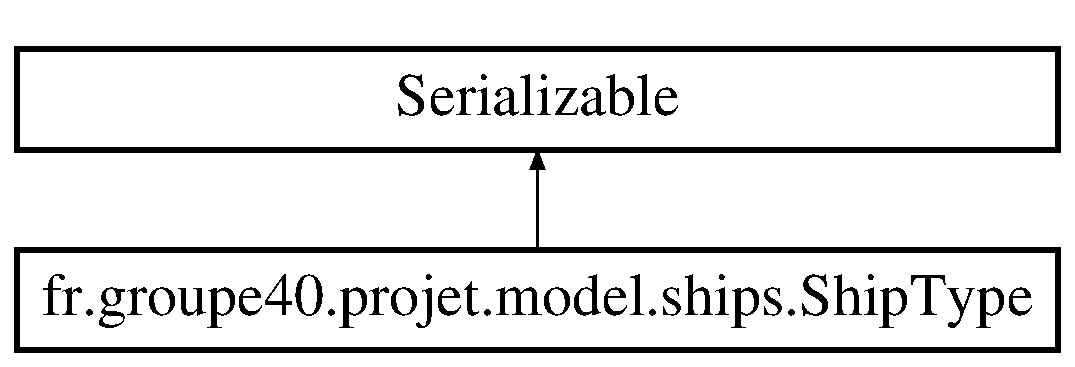
\includegraphics[height=2.000000cm]{classfr_1_1groupe40_1_1projet_1_1model_1_1ships_1_1_ship_type}
\end{center}
\end{figure}
\subsection*{Protected Attributes}
\begin{DoxyCompactItemize}
\item 
\mbox{\Hypertarget{classfr_1_1groupe40_1_1projet_1_1model_1_1ships_1_1_ship_type_a1b9a8c6f8feb78937126e77eee96fa4f}\label{classfr_1_1groupe40_1_1projet_1_1model_1_1ships_1_1_ship_type_a1b9a8c6f8feb78937126e77eee96fa4f}} 
double {\bfseries speed}
\end{DoxyCompactItemize}


The documentation for this class was generated from the following file\+:\begin{DoxyCompactItemize}
\item 
src/fr/groupe40/projet/model/ships/Ship\+Type.\+java\end{DoxyCompactItemize}

\hypertarget{classfr_1_1groupe40_1_1projet_1_1model_1_1_sprite}{}\section{fr.\+groupe40.\+projet.\+model.\+Sprite Class Reference}
\label{classfr_1_1groupe40_1_1projet_1_1model_1_1_sprite}\index{fr.\+groupe40.\+projet.\+model.\+Sprite@{fr.\+groupe40.\+projet.\+model.\+Sprite}}
Inheritance diagram for fr.\+groupe40.\+projet.\+model.\+Sprite\+:\begin{figure}[H]
\begin{center}
\leavevmode
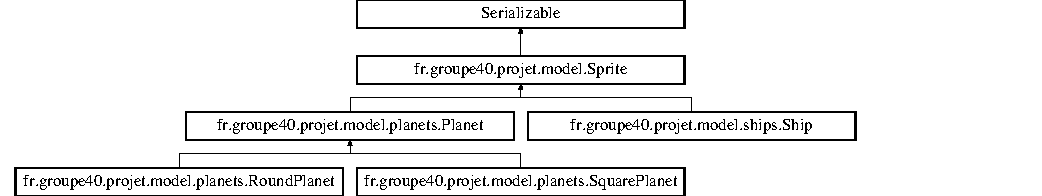
\includegraphics[height=2.638398cm]{classfr_1_1groupe40_1_1projet_1_1model_1_1_sprite}
\end{center}
\end{figure}
\subsection*{Public Member Functions}
\begin{DoxyCompactItemize}
\item 
\hyperlink{classfr_1_1groupe40_1_1projet_1_1model_1_1_sprite_acbe678213b404fd8ae1a77fe274fdca8}{Sprite} (String path, \hyperlink{classfr_1_1groupe40_1_1projet_1_1client_1_1_user}{User} ruler, boolean is\+Planet)
\begin{DoxyCompactList}\small\item\em Create a sprite from an image path, a ruler and if its a planets or not. \end{DoxyCompactList}\item 
\mbox{\Hypertarget{classfr_1_1groupe40_1_1projet_1_1model_1_1_sprite_a762bbcf4f03eecab8de2b05aa19a103a}\label{classfr_1_1groupe40_1_1projet_1_1model_1_1_sprite_a762bbcf4f03eecab8de2b05aa19a103a}} 
void \hyperlink{classfr_1_1groupe40_1_1projet_1_1model_1_1_sprite_a762bbcf4f03eecab8de2b05aa19a103a}{update\+Image} ()
\begin{DoxyCompactList}\small\item\em Update the image linked to a sprite. \end{DoxyCompactList}\item 
void \hyperlink{classfr_1_1groupe40_1_1projet_1_1model_1_1_sprite_ab3b2649df13b98ba229c292328e31b25}{set\+Position} (int x, int y)
\begin{DoxyCompactList}\small\item\em Set the x and y position of a sprite. \end{DoxyCompactList}\item 
double \hyperlink{classfr_1_1groupe40_1_1projet_1_1model_1_1_sprite_a4907c1229ac5b6a614e880649240ea7b}{distance} (double x, double y)
\begin{DoxyCompactList}\small\item\em Return the distance between a sprite and a 2d coord. \end{DoxyCompactList}\item 
double \hyperlink{classfr_1_1groupe40_1_1projet_1_1model_1_1_sprite_aa74fb93449c20a79f16edca9a7ae9482}{distance} (double x1, double y1, double x2, double y2)
\begin{DoxyCompactList}\small\item\em Return the distance between 2 dots. \end{DoxyCompactList}\item 
double \hyperlink{classfr_1_1groupe40_1_1projet_1_1model_1_1_sprite_af42e0eb11d2408ca1f4bbb17164e3b24}{distance} (\hyperlink{classfr_1_1groupe40_1_1projet_1_1model_1_1_sprite}{Sprite} p)
\begin{DoxyCompactList}\small\item\em Calculate the distance between 2 sprites. \end{DoxyCompactList}\item 
\mbox{\Hypertarget{classfr_1_1groupe40_1_1projet_1_1model_1_1_sprite_a38a7ee4fb45129e891b8a78a120ffe94}\label{classfr_1_1groupe40_1_1projet_1_1model_1_1_sprite_a38a7ee4fb45129e891b8a78a120ffe94}} 
void \hyperlink{classfr_1_1groupe40_1_1projet_1_1model_1_1_sprite_a38a7ee4fb45129e891b8a78a120ffe94}{validate\+Position} ()
\begin{DoxyCompactList}\small\item\em Verify if a sprite is not out of bounds. \end{DoxyCompactList}\item 
boolean \hyperlink{classfr_1_1groupe40_1_1projet_1_1model_1_1_sprite_a2a5da521a659f398efee6f2b0a45aa51}{intersect\+Circle} (double x\+\_\+left, double y\+\_\+top, double x\+\_\+right, double y\+\_\+bottom)
\begin{DoxyCompactList}\small\item\em Check if a rectangle intersect a circle. \end{DoxyCompactList}\item 
boolean \hyperlink{classfr_1_1groupe40_1_1projet_1_1model_1_1_sprite_a87346b18a5d8370e1f0634011698675b}{intersect\+Circle} (\hyperlink{classfr_1_1groupe40_1_1projet_1_1model_1_1_sprite}{Sprite} p)
\begin{DoxyCompactList}\small\item\em Check if a sprite intersect another circle from a sprite In fact, we\textquotesingle{}re generating a circle around a sprite to check the distance between each others. \end{DoxyCompactList}\item 
boolean \hyperlink{classfr_1_1groupe40_1_1projet_1_1model_1_1_sprite_a7c826b664373d244725751f74c057b12}{is\+Inside} (double x, double y, double width, double height)
\begin{DoxyCompactList}\small\item\em Check if a rectangle is inside another. \end{DoxyCompactList}\item 
boolean \hyperlink{classfr_1_1groupe40_1_1projet_1_1model_1_1_sprite_a2c39c997fa632f4d90807fdaa3a4a9b4}{is\+Inside} (\hyperlink{classfr_1_1groupe40_1_1projet_1_1model_1_1_sprite}{Sprite} s)
\begin{DoxyCompactList}\small\item\em Check if a sprite directly intersect another one. \end{DoxyCompactList}\item 
void \hyperlink{classfr_1_1groupe40_1_1projet_1_1model_1_1_sprite_a12305126f539c9403a9bb03a861aa9c0}{set\+Position} (double x, double y)
\begin{DoxyCompactList}\small\item\em Set the position of a sprite then validate his position. \end{DoxyCompactList}\item 
void \hyperlink{classfr_1_1groupe40_1_1projet_1_1model_1_1_sprite_adaa6c20253be22213e199b90d709f275}{render} (Graphics\+Context gc)
\begin{DoxyCompactList}\small\item\em Render the image of this sprite. \end{DoxyCompactList}\item 
\mbox{\Hypertarget{classfr_1_1groupe40_1_1projet_1_1model_1_1_sprite_a171e3b2a9d38864f6f4a5fef3e8efe49}\label{classfr_1_1groupe40_1_1projet_1_1model_1_1_sprite_a171e3b2a9d38864f6f4a5fef3e8efe49}} 
String \hyperlink{classfr_1_1groupe40_1_1projet_1_1model_1_1_sprite_a171e3b2a9d38864f6f4a5fef3e8efe49}{to\+String} ()
\begin{DoxyCompactList}\small\item\em convert the object to string with his 2D position \end{DoxyCompactList}\item 
Image \hyperlink{classfr_1_1groupe40_1_1projet_1_1model_1_1_sprite_ae978c58649b232749722a2c2c86e1f0d}{get\+Image} ()
\item 
void \hyperlink{classfr_1_1groupe40_1_1projet_1_1model_1_1_sprite_a79c8fe34e9f81804079ca381b589f6e3}{set\+Image} (Image image)
\item 
String \hyperlink{classfr_1_1groupe40_1_1projet_1_1model_1_1_sprite_a208906f75c02531120b4d0c78c59e7f9}{get\+Img\+\_\+path} ()
\item 
void \hyperlink{classfr_1_1groupe40_1_1projet_1_1model_1_1_sprite_a6d246968ec03152ee63d12696c6cd9a4}{set\+Img\+\_\+path} (String img\+\_\+path)
\item 
double \hyperlink{classfr_1_1groupe40_1_1projet_1_1model_1_1_sprite_a9c9d69c95176ab9663f7b2beb64d6a2d}{width} ()
\item 
void \hyperlink{classfr_1_1groupe40_1_1projet_1_1model_1_1_sprite_a600096893822f1625075033719653eb9}{set\+Width} (double width)
\item 
double \hyperlink{classfr_1_1groupe40_1_1projet_1_1model_1_1_sprite_aabcca84219036d2102c9308fbb7ed178}{height} ()
\item 
void \hyperlink{classfr_1_1groupe40_1_1projet_1_1model_1_1_sprite_a420a31eed0b03963f576f6f85678e786}{set\+Height} (double height)
\item 
double \hyperlink{classfr_1_1groupe40_1_1projet_1_1model_1_1_sprite_a4d47964ca6de87bfd8f604f76228d19e}{getX} ()
\item 
void \hyperlink{classfr_1_1groupe40_1_1projet_1_1model_1_1_sprite_ac4eeeae6da38d81fb352dff02446e10e}{setX} (double x)
\item 
double \hyperlink{classfr_1_1groupe40_1_1projet_1_1model_1_1_sprite_ac1741b13dc3196aef8d15dd34d7ad148}{getY} ()
\item 
void \hyperlink{classfr_1_1groupe40_1_1projet_1_1model_1_1_sprite_a95a46d20a0736d4d9138c2e865fd0c1d}{setY} (double y)
\item 
double \hyperlink{classfr_1_1groupe40_1_1projet_1_1model_1_1_sprite_a7cd8a84c600d9b6c4d1a274dde323798}{get\+MaxX} ()
\item 
void \hyperlink{classfr_1_1groupe40_1_1projet_1_1model_1_1_sprite_a078737a859b0efa95946ecd96122bf9d}{set\+MaxX} (double maxX)
\item 
double \hyperlink{classfr_1_1groupe40_1_1projet_1_1model_1_1_sprite_a34a9046a79de7a8eb37d7eac872c8266}{get\+MaxY} ()
\item 
void \hyperlink{classfr_1_1groupe40_1_1projet_1_1model_1_1_sprite_a27bc3277ad1dd83dd34dd493cc854d4d}{set\+MaxY} (double maxY)
\item 
double \hyperlink{classfr_1_1groupe40_1_1projet_1_1model_1_1_sprite_ac23be69d6ef6bd9edb52e2e2afe49a79}{get\+MinX} ()
\item 
void \hyperlink{classfr_1_1groupe40_1_1projet_1_1model_1_1_sprite_a41cb9d59bc9711494a898f6a6ffca6a1}{set\+MinX} (double minX)
\item 
double \hyperlink{classfr_1_1groupe40_1_1projet_1_1model_1_1_sprite_acea4638f2af1049a66467d338b587287}{get\+MinY} ()
\item 
void \hyperlink{classfr_1_1groupe40_1_1projet_1_1model_1_1_sprite_af3554a7ce1504869fecf6170e62996ab}{set\+MinY} (double minY)
\item 
\hyperlink{classfr_1_1groupe40_1_1projet_1_1client_1_1_user}{User} \hyperlink{classfr_1_1groupe40_1_1projet_1_1model_1_1_sprite_aeac1692f370ceb45e87685b3a97a5123}{get\+Ruler} ()
\item 
void \hyperlink{classfr_1_1groupe40_1_1projet_1_1model_1_1_sprite_a5821b7c642529666d029deb409d41457}{set\+Ruler} (\hyperlink{classfr_1_1groupe40_1_1projet_1_1client_1_1_user}{User} ruler)
\end{DoxyCompactItemize}


\subsection{Detailed Description}
\begin{DoxyAuthor}{Author}
Jordane Masson 

Sarah Portejoie 
\end{DoxyAuthor}


\subsection{Constructor \& Destructor Documentation}
\mbox{\Hypertarget{classfr_1_1groupe40_1_1projet_1_1model_1_1_sprite_acbe678213b404fd8ae1a77fe274fdca8}\label{classfr_1_1groupe40_1_1projet_1_1model_1_1_sprite_acbe678213b404fd8ae1a77fe274fdca8}} 
\index{fr\+::groupe40\+::projet\+::model\+::\+Sprite@{fr\+::groupe40\+::projet\+::model\+::\+Sprite}!Sprite@{Sprite}}
\index{Sprite@{Sprite}!fr\+::groupe40\+::projet\+::model\+::\+Sprite@{fr\+::groupe40\+::projet\+::model\+::\+Sprite}}
\subsubsection{\texorpdfstring{Sprite()}{Sprite()}}
{\footnotesize\ttfamily fr.\+groupe40.\+projet.\+model.\+Sprite.\+Sprite (\begin{DoxyParamCaption}\item[{String}]{path,  }\item[{\hyperlink{classfr_1_1groupe40_1_1projet_1_1client_1_1_user}{User}}]{ruler,  }\item[{boolean}]{is\+Planet }\end{DoxyParamCaption})}



Create a sprite from an image path, a ruler and if its a planets or not. 


\begin{DoxyParams}{Parameters}
{\em path} & Path to the image file \\
\hline
{\em ruler} & Ruler of this sprite \\
\hline
{\em is\+Planet} & Its a planet or not \\
\hline
\end{DoxyParams}


\subsection{Member Function Documentation}
\mbox{\Hypertarget{classfr_1_1groupe40_1_1projet_1_1model_1_1_sprite_a4907c1229ac5b6a614e880649240ea7b}\label{classfr_1_1groupe40_1_1projet_1_1model_1_1_sprite_a4907c1229ac5b6a614e880649240ea7b}} 
\index{fr\+::groupe40\+::projet\+::model\+::\+Sprite@{fr\+::groupe40\+::projet\+::model\+::\+Sprite}!distance@{distance}}
\index{distance@{distance}!fr\+::groupe40\+::projet\+::model\+::\+Sprite@{fr\+::groupe40\+::projet\+::model\+::\+Sprite}}
\subsubsection{\texorpdfstring{distance()}{distance()}\hspace{0.1cm}{\footnotesize\ttfamily [1/3]}}
{\footnotesize\ttfamily double fr.\+groupe40.\+projet.\+model.\+Sprite.\+distance (\begin{DoxyParamCaption}\item[{double}]{x,  }\item[{double}]{y }\end{DoxyParamCaption})}



Return the distance between a sprite and a 2d coord. 


\begin{DoxyParams}{Parameters}
{\em x} & \\
\hline
{\em y} & \\
\hline
\end{DoxyParams}
\begin{DoxyReturn}{Returns}
Distance between those 2 positions 
\end{DoxyReturn}
\mbox{\Hypertarget{classfr_1_1groupe40_1_1projet_1_1model_1_1_sprite_aa74fb93449c20a79f16edca9a7ae9482}\label{classfr_1_1groupe40_1_1projet_1_1model_1_1_sprite_aa74fb93449c20a79f16edca9a7ae9482}} 
\index{fr\+::groupe40\+::projet\+::model\+::\+Sprite@{fr\+::groupe40\+::projet\+::model\+::\+Sprite}!distance@{distance}}
\index{distance@{distance}!fr\+::groupe40\+::projet\+::model\+::\+Sprite@{fr\+::groupe40\+::projet\+::model\+::\+Sprite}}
\subsubsection{\texorpdfstring{distance()}{distance()}\hspace{0.1cm}{\footnotesize\ttfamily [2/3]}}
{\footnotesize\ttfamily double fr.\+groupe40.\+projet.\+model.\+Sprite.\+distance (\begin{DoxyParamCaption}\item[{double}]{x1,  }\item[{double}]{y1,  }\item[{double}]{x2,  }\item[{double}]{y2 }\end{DoxyParamCaption})}



Return the distance between 2 dots. 


\begin{DoxyParams}{Parameters}
{\em x1} & \\
\hline
{\em y1} & \\
\hline
{\em x2} & \\
\hline
{\em y2} & \\
\hline
\end{DoxyParams}
\begin{DoxyReturn}{Returns}
A distance 
\end{DoxyReturn}
\mbox{\Hypertarget{classfr_1_1groupe40_1_1projet_1_1model_1_1_sprite_af42e0eb11d2408ca1f4bbb17164e3b24}\label{classfr_1_1groupe40_1_1projet_1_1model_1_1_sprite_af42e0eb11d2408ca1f4bbb17164e3b24}} 
\index{fr\+::groupe40\+::projet\+::model\+::\+Sprite@{fr\+::groupe40\+::projet\+::model\+::\+Sprite}!distance@{distance}}
\index{distance@{distance}!fr\+::groupe40\+::projet\+::model\+::\+Sprite@{fr\+::groupe40\+::projet\+::model\+::\+Sprite}}
\subsubsection{\texorpdfstring{distance()}{distance()}\hspace{0.1cm}{\footnotesize\ttfamily [3/3]}}
{\footnotesize\ttfamily double fr.\+groupe40.\+projet.\+model.\+Sprite.\+distance (\begin{DoxyParamCaption}\item[{\hyperlink{classfr_1_1groupe40_1_1projet_1_1model_1_1_sprite}{Sprite}}]{p }\end{DoxyParamCaption})}



Calculate the distance between 2 sprites. 


\begin{DoxyParams}{Parameters}
{\em p} & Second sprite to compare with \\
\hline
\end{DoxyParams}
\begin{DoxyReturn}{Returns}
The distance 
\end{DoxyReturn}
\mbox{\Hypertarget{classfr_1_1groupe40_1_1projet_1_1model_1_1_sprite_ae978c58649b232749722a2c2c86e1f0d}\label{classfr_1_1groupe40_1_1projet_1_1model_1_1_sprite_ae978c58649b232749722a2c2c86e1f0d}} 
\index{fr\+::groupe40\+::projet\+::model\+::\+Sprite@{fr\+::groupe40\+::projet\+::model\+::\+Sprite}!get\+Image@{get\+Image}}
\index{get\+Image@{get\+Image}!fr\+::groupe40\+::projet\+::model\+::\+Sprite@{fr\+::groupe40\+::projet\+::model\+::\+Sprite}}
\subsubsection{\texorpdfstring{get\+Image()}{getImage()}}
{\footnotesize\ttfamily Image fr.\+groupe40.\+projet.\+model.\+Sprite.\+get\+Image (\begin{DoxyParamCaption}{ }\end{DoxyParamCaption})}

\begin{DoxyReturn}{Returns}
the image 
\end{DoxyReturn}
\mbox{\Hypertarget{classfr_1_1groupe40_1_1projet_1_1model_1_1_sprite_a208906f75c02531120b4d0c78c59e7f9}\label{classfr_1_1groupe40_1_1projet_1_1model_1_1_sprite_a208906f75c02531120b4d0c78c59e7f9}} 
\index{fr\+::groupe40\+::projet\+::model\+::\+Sprite@{fr\+::groupe40\+::projet\+::model\+::\+Sprite}!get\+Img\+\_\+path@{get\+Img\+\_\+path}}
\index{get\+Img\+\_\+path@{get\+Img\+\_\+path}!fr\+::groupe40\+::projet\+::model\+::\+Sprite@{fr\+::groupe40\+::projet\+::model\+::\+Sprite}}
\subsubsection{\texorpdfstring{get\+Img\+\_\+path()}{getImg\_path()}}
{\footnotesize\ttfamily String fr.\+groupe40.\+projet.\+model.\+Sprite.\+get\+Img\+\_\+path (\begin{DoxyParamCaption}{ }\end{DoxyParamCaption})}

\begin{DoxyReturn}{Returns}
the img\+\_\+path 
\end{DoxyReturn}
\mbox{\Hypertarget{classfr_1_1groupe40_1_1projet_1_1model_1_1_sprite_a7cd8a84c600d9b6c4d1a274dde323798}\label{classfr_1_1groupe40_1_1projet_1_1model_1_1_sprite_a7cd8a84c600d9b6c4d1a274dde323798}} 
\index{fr\+::groupe40\+::projet\+::model\+::\+Sprite@{fr\+::groupe40\+::projet\+::model\+::\+Sprite}!get\+MaxX@{get\+MaxX}}
\index{get\+MaxX@{get\+MaxX}!fr\+::groupe40\+::projet\+::model\+::\+Sprite@{fr\+::groupe40\+::projet\+::model\+::\+Sprite}}
\subsubsection{\texorpdfstring{get\+Max\+X()}{getMaxX()}}
{\footnotesize\ttfamily double fr.\+groupe40.\+projet.\+model.\+Sprite.\+get\+MaxX (\begin{DoxyParamCaption}{ }\end{DoxyParamCaption})}

\begin{DoxyReturn}{Returns}
the maxX 
\end{DoxyReturn}
\mbox{\Hypertarget{classfr_1_1groupe40_1_1projet_1_1model_1_1_sprite_a34a9046a79de7a8eb37d7eac872c8266}\label{classfr_1_1groupe40_1_1projet_1_1model_1_1_sprite_a34a9046a79de7a8eb37d7eac872c8266}} 
\index{fr\+::groupe40\+::projet\+::model\+::\+Sprite@{fr\+::groupe40\+::projet\+::model\+::\+Sprite}!get\+MaxY@{get\+MaxY}}
\index{get\+MaxY@{get\+MaxY}!fr\+::groupe40\+::projet\+::model\+::\+Sprite@{fr\+::groupe40\+::projet\+::model\+::\+Sprite}}
\subsubsection{\texorpdfstring{get\+Max\+Y()}{getMaxY()}}
{\footnotesize\ttfamily double fr.\+groupe40.\+projet.\+model.\+Sprite.\+get\+MaxY (\begin{DoxyParamCaption}{ }\end{DoxyParamCaption})}

\begin{DoxyReturn}{Returns}
the maxY 
\end{DoxyReturn}
\mbox{\Hypertarget{classfr_1_1groupe40_1_1projet_1_1model_1_1_sprite_ac23be69d6ef6bd9edb52e2e2afe49a79}\label{classfr_1_1groupe40_1_1projet_1_1model_1_1_sprite_ac23be69d6ef6bd9edb52e2e2afe49a79}} 
\index{fr\+::groupe40\+::projet\+::model\+::\+Sprite@{fr\+::groupe40\+::projet\+::model\+::\+Sprite}!get\+MinX@{get\+MinX}}
\index{get\+MinX@{get\+MinX}!fr\+::groupe40\+::projet\+::model\+::\+Sprite@{fr\+::groupe40\+::projet\+::model\+::\+Sprite}}
\subsubsection{\texorpdfstring{get\+Min\+X()}{getMinX()}}
{\footnotesize\ttfamily double fr.\+groupe40.\+projet.\+model.\+Sprite.\+get\+MinX (\begin{DoxyParamCaption}{ }\end{DoxyParamCaption})}

\begin{DoxyReturn}{Returns}
the minX 
\end{DoxyReturn}
\mbox{\Hypertarget{classfr_1_1groupe40_1_1projet_1_1model_1_1_sprite_acea4638f2af1049a66467d338b587287}\label{classfr_1_1groupe40_1_1projet_1_1model_1_1_sprite_acea4638f2af1049a66467d338b587287}} 
\index{fr\+::groupe40\+::projet\+::model\+::\+Sprite@{fr\+::groupe40\+::projet\+::model\+::\+Sprite}!get\+MinY@{get\+MinY}}
\index{get\+MinY@{get\+MinY}!fr\+::groupe40\+::projet\+::model\+::\+Sprite@{fr\+::groupe40\+::projet\+::model\+::\+Sprite}}
\subsubsection{\texorpdfstring{get\+Min\+Y()}{getMinY()}}
{\footnotesize\ttfamily double fr.\+groupe40.\+projet.\+model.\+Sprite.\+get\+MinY (\begin{DoxyParamCaption}{ }\end{DoxyParamCaption})}

\begin{DoxyReturn}{Returns}
the minY 
\end{DoxyReturn}
\mbox{\Hypertarget{classfr_1_1groupe40_1_1projet_1_1model_1_1_sprite_aeac1692f370ceb45e87685b3a97a5123}\label{classfr_1_1groupe40_1_1projet_1_1model_1_1_sprite_aeac1692f370ceb45e87685b3a97a5123}} 
\index{fr\+::groupe40\+::projet\+::model\+::\+Sprite@{fr\+::groupe40\+::projet\+::model\+::\+Sprite}!get\+Ruler@{get\+Ruler}}
\index{get\+Ruler@{get\+Ruler}!fr\+::groupe40\+::projet\+::model\+::\+Sprite@{fr\+::groupe40\+::projet\+::model\+::\+Sprite}}
\subsubsection{\texorpdfstring{get\+Ruler()}{getRuler()}}
{\footnotesize\ttfamily \hyperlink{classfr_1_1groupe40_1_1projet_1_1client_1_1_user}{User} fr.\+groupe40.\+projet.\+model.\+Sprite.\+get\+Ruler (\begin{DoxyParamCaption}{ }\end{DoxyParamCaption})}

\begin{DoxyReturn}{Returns}
the ruler 
\end{DoxyReturn}
\mbox{\Hypertarget{classfr_1_1groupe40_1_1projet_1_1model_1_1_sprite_a4d47964ca6de87bfd8f604f76228d19e}\label{classfr_1_1groupe40_1_1projet_1_1model_1_1_sprite_a4d47964ca6de87bfd8f604f76228d19e}} 
\index{fr\+::groupe40\+::projet\+::model\+::\+Sprite@{fr\+::groupe40\+::projet\+::model\+::\+Sprite}!getX@{getX}}
\index{getX@{getX}!fr\+::groupe40\+::projet\+::model\+::\+Sprite@{fr\+::groupe40\+::projet\+::model\+::\+Sprite}}
\subsubsection{\texorpdfstring{get\+X()}{getX()}}
{\footnotesize\ttfamily double fr.\+groupe40.\+projet.\+model.\+Sprite.\+getX (\begin{DoxyParamCaption}{ }\end{DoxyParamCaption})}

\begin{DoxyReturn}{Returns}
the x 
\end{DoxyReturn}
\mbox{\Hypertarget{classfr_1_1groupe40_1_1projet_1_1model_1_1_sprite_ac1741b13dc3196aef8d15dd34d7ad148}\label{classfr_1_1groupe40_1_1projet_1_1model_1_1_sprite_ac1741b13dc3196aef8d15dd34d7ad148}} 
\index{fr\+::groupe40\+::projet\+::model\+::\+Sprite@{fr\+::groupe40\+::projet\+::model\+::\+Sprite}!getY@{getY}}
\index{getY@{getY}!fr\+::groupe40\+::projet\+::model\+::\+Sprite@{fr\+::groupe40\+::projet\+::model\+::\+Sprite}}
\subsubsection{\texorpdfstring{get\+Y()}{getY()}}
{\footnotesize\ttfamily double fr.\+groupe40.\+projet.\+model.\+Sprite.\+getY (\begin{DoxyParamCaption}{ }\end{DoxyParamCaption})}

\begin{DoxyReturn}{Returns}
the y 
\end{DoxyReturn}
\mbox{\Hypertarget{classfr_1_1groupe40_1_1projet_1_1model_1_1_sprite_aabcca84219036d2102c9308fbb7ed178}\label{classfr_1_1groupe40_1_1projet_1_1model_1_1_sprite_aabcca84219036d2102c9308fbb7ed178}} 
\index{fr\+::groupe40\+::projet\+::model\+::\+Sprite@{fr\+::groupe40\+::projet\+::model\+::\+Sprite}!height@{height}}
\index{height@{height}!fr\+::groupe40\+::projet\+::model\+::\+Sprite@{fr\+::groupe40\+::projet\+::model\+::\+Sprite}}
\subsubsection{\texorpdfstring{height()}{height()}}
{\footnotesize\ttfamily double fr.\+groupe40.\+projet.\+model.\+Sprite.\+height (\begin{DoxyParamCaption}{ }\end{DoxyParamCaption})}

\begin{DoxyReturn}{Returns}
the height 
\end{DoxyReturn}
\mbox{\Hypertarget{classfr_1_1groupe40_1_1projet_1_1model_1_1_sprite_a2a5da521a659f398efee6f2b0a45aa51}\label{classfr_1_1groupe40_1_1projet_1_1model_1_1_sprite_a2a5da521a659f398efee6f2b0a45aa51}} 
\index{fr\+::groupe40\+::projet\+::model\+::\+Sprite@{fr\+::groupe40\+::projet\+::model\+::\+Sprite}!intersect\+Circle@{intersect\+Circle}}
\index{intersect\+Circle@{intersect\+Circle}!fr\+::groupe40\+::projet\+::model\+::\+Sprite@{fr\+::groupe40\+::projet\+::model\+::\+Sprite}}
\subsubsection{\texorpdfstring{intersect\+Circle()}{intersectCircle()}\hspace{0.1cm}{\footnotesize\ttfamily [1/2]}}
{\footnotesize\ttfamily boolean fr.\+groupe40.\+projet.\+model.\+Sprite.\+intersect\+Circle (\begin{DoxyParamCaption}\item[{double}]{x\+\_\+left,  }\item[{double}]{y\+\_\+top,  }\item[{double}]{x\+\_\+right,  }\item[{double}]{y\+\_\+bottom }\end{DoxyParamCaption})}



Check if a rectangle intersect a circle. 


\begin{DoxyParams}{Parameters}
{\em x\+\_\+left} & \\
\hline
{\em y\+\_\+top} & \\
\hline
{\em x\+\_\+right} & \\
\hline
{\em y\+\_\+bottom} & \\
\hline
\end{DoxyParams}
\begin{DoxyReturn}{Returns}
true if there s a collision, else false 
\end{DoxyReturn}
\mbox{\Hypertarget{classfr_1_1groupe40_1_1projet_1_1model_1_1_sprite_a87346b18a5d8370e1f0634011698675b}\label{classfr_1_1groupe40_1_1projet_1_1model_1_1_sprite_a87346b18a5d8370e1f0634011698675b}} 
\index{fr\+::groupe40\+::projet\+::model\+::\+Sprite@{fr\+::groupe40\+::projet\+::model\+::\+Sprite}!intersect\+Circle@{intersect\+Circle}}
\index{intersect\+Circle@{intersect\+Circle}!fr\+::groupe40\+::projet\+::model\+::\+Sprite@{fr\+::groupe40\+::projet\+::model\+::\+Sprite}}
\subsubsection{\texorpdfstring{intersect\+Circle()}{intersectCircle()}\hspace{0.1cm}{\footnotesize\ttfamily [2/2]}}
{\footnotesize\ttfamily boolean fr.\+groupe40.\+projet.\+model.\+Sprite.\+intersect\+Circle (\begin{DoxyParamCaption}\item[{\hyperlink{classfr_1_1groupe40_1_1projet_1_1model_1_1_sprite}{Sprite}}]{p }\end{DoxyParamCaption})}



Check if a sprite intersect another circle from a sprite In fact, we\textquotesingle{}re generating a circle around a sprite to check the distance between each others. 


\begin{DoxyParams}{Parameters}
{\em p} & a sprite \\
\hline
\end{DoxyParams}
\begin{DoxyReturn}{Returns}
true if the sprite is in the circle else false 
\end{DoxyReturn}
\mbox{\Hypertarget{classfr_1_1groupe40_1_1projet_1_1model_1_1_sprite_a7c826b664373d244725751f74c057b12}\label{classfr_1_1groupe40_1_1projet_1_1model_1_1_sprite_a7c826b664373d244725751f74c057b12}} 
\index{fr\+::groupe40\+::projet\+::model\+::\+Sprite@{fr\+::groupe40\+::projet\+::model\+::\+Sprite}!is\+Inside@{is\+Inside}}
\index{is\+Inside@{is\+Inside}!fr\+::groupe40\+::projet\+::model\+::\+Sprite@{fr\+::groupe40\+::projet\+::model\+::\+Sprite}}
\subsubsection{\texorpdfstring{is\+Inside()}{isInside()}\hspace{0.1cm}{\footnotesize\ttfamily [1/2]}}
{\footnotesize\ttfamily boolean fr.\+groupe40.\+projet.\+model.\+Sprite.\+is\+Inside (\begin{DoxyParamCaption}\item[{double}]{x,  }\item[{double}]{y,  }\item[{double}]{width,  }\item[{double}]{height }\end{DoxyParamCaption})}



Check if a rectangle is inside another. 


\begin{DoxyParams}{Parameters}
{\em x} & the x-\/top corner \\
\hline
{\em y} & the y-\/top corner \\
\hline
{\em width} & the width of the rectangle \\
\hline
{\em height} & the height of the rectangle \\
\hline
\end{DoxyParams}
\begin{DoxyReturn}{Returns}
true if inside else false 
\end{DoxyReturn}
\mbox{\Hypertarget{classfr_1_1groupe40_1_1projet_1_1model_1_1_sprite_a2c39c997fa632f4d90807fdaa3a4a9b4}\label{classfr_1_1groupe40_1_1projet_1_1model_1_1_sprite_a2c39c997fa632f4d90807fdaa3a4a9b4}} 
\index{fr\+::groupe40\+::projet\+::model\+::\+Sprite@{fr\+::groupe40\+::projet\+::model\+::\+Sprite}!is\+Inside@{is\+Inside}}
\index{is\+Inside@{is\+Inside}!fr\+::groupe40\+::projet\+::model\+::\+Sprite@{fr\+::groupe40\+::projet\+::model\+::\+Sprite}}
\subsubsection{\texorpdfstring{is\+Inside()}{isInside()}\hspace{0.1cm}{\footnotesize\ttfamily [2/2]}}
{\footnotesize\ttfamily boolean fr.\+groupe40.\+projet.\+model.\+Sprite.\+is\+Inside (\begin{DoxyParamCaption}\item[{\hyperlink{classfr_1_1groupe40_1_1projet_1_1model_1_1_sprite}{Sprite}}]{s }\end{DoxyParamCaption})}



Check if a sprite directly intersect another one. 


\begin{DoxyParams}{Parameters}
{\em s} & the sprite to compare with \\
\hline
\end{DoxyParams}
\begin{DoxyReturn}{Returns}
true if the sprite is inside, else false 
\end{DoxyReturn}
\mbox{\Hypertarget{classfr_1_1groupe40_1_1projet_1_1model_1_1_sprite_adaa6c20253be22213e199b90d709f275}\label{classfr_1_1groupe40_1_1projet_1_1model_1_1_sprite_adaa6c20253be22213e199b90d709f275}} 
\index{fr\+::groupe40\+::projet\+::model\+::\+Sprite@{fr\+::groupe40\+::projet\+::model\+::\+Sprite}!render@{render}}
\index{render@{render}!fr\+::groupe40\+::projet\+::model\+::\+Sprite@{fr\+::groupe40\+::projet\+::model\+::\+Sprite}}
\subsubsection{\texorpdfstring{render()}{render()}}
{\footnotesize\ttfamily void fr.\+groupe40.\+projet.\+model.\+Sprite.\+render (\begin{DoxyParamCaption}\item[{Graphics\+Context}]{gc }\end{DoxyParamCaption})}



Render the image of this sprite. 


\begin{DoxyParams}{Parameters}
{\em gc} & \\
\hline
\end{DoxyParams}
\mbox{\Hypertarget{classfr_1_1groupe40_1_1projet_1_1model_1_1_sprite_a420a31eed0b03963f576f6f85678e786}\label{classfr_1_1groupe40_1_1projet_1_1model_1_1_sprite_a420a31eed0b03963f576f6f85678e786}} 
\index{fr\+::groupe40\+::projet\+::model\+::\+Sprite@{fr\+::groupe40\+::projet\+::model\+::\+Sprite}!set\+Height@{set\+Height}}
\index{set\+Height@{set\+Height}!fr\+::groupe40\+::projet\+::model\+::\+Sprite@{fr\+::groupe40\+::projet\+::model\+::\+Sprite}}
\subsubsection{\texorpdfstring{set\+Height()}{setHeight()}}
{\footnotesize\ttfamily void fr.\+groupe40.\+projet.\+model.\+Sprite.\+set\+Height (\begin{DoxyParamCaption}\item[{double}]{height }\end{DoxyParamCaption})}


\begin{DoxyParams}{Parameters}
{\em height} & the height to set \\
\hline
\end{DoxyParams}
\mbox{\Hypertarget{classfr_1_1groupe40_1_1projet_1_1model_1_1_sprite_a79c8fe34e9f81804079ca381b589f6e3}\label{classfr_1_1groupe40_1_1projet_1_1model_1_1_sprite_a79c8fe34e9f81804079ca381b589f6e3}} 
\index{fr\+::groupe40\+::projet\+::model\+::\+Sprite@{fr\+::groupe40\+::projet\+::model\+::\+Sprite}!set\+Image@{set\+Image}}
\index{set\+Image@{set\+Image}!fr\+::groupe40\+::projet\+::model\+::\+Sprite@{fr\+::groupe40\+::projet\+::model\+::\+Sprite}}
\subsubsection{\texorpdfstring{set\+Image()}{setImage()}}
{\footnotesize\ttfamily void fr.\+groupe40.\+projet.\+model.\+Sprite.\+set\+Image (\begin{DoxyParamCaption}\item[{Image}]{image }\end{DoxyParamCaption})}


\begin{DoxyParams}{Parameters}
{\em image} & the image to set \\
\hline
\end{DoxyParams}
\mbox{\Hypertarget{classfr_1_1groupe40_1_1projet_1_1model_1_1_sprite_a6d246968ec03152ee63d12696c6cd9a4}\label{classfr_1_1groupe40_1_1projet_1_1model_1_1_sprite_a6d246968ec03152ee63d12696c6cd9a4}} 
\index{fr\+::groupe40\+::projet\+::model\+::\+Sprite@{fr\+::groupe40\+::projet\+::model\+::\+Sprite}!set\+Img\+\_\+path@{set\+Img\+\_\+path}}
\index{set\+Img\+\_\+path@{set\+Img\+\_\+path}!fr\+::groupe40\+::projet\+::model\+::\+Sprite@{fr\+::groupe40\+::projet\+::model\+::\+Sprite}}
\subsubsection{\texorpdfstring{set\+Img\+\_\+path()}{setImg\_path()}}
{\footnotesize\ttfamily void fr.\+groupe40.\+projet.\+model.\+Sprite.\+set\+Img\+\_\+path (\begin{DoxyParamCaption}\item[{String}]{img\+\_\+path }\end{DoxyParamCaption})}


\begin{DoxyParams}{Parameters}
{\em img\+\_\+path} & the img\+\_\+path to set \\
\hline
\end{DoxyParams}
\mbox{\Hypertarget{classfr_1_1groupe40_1_1projet_1_1model_1_1_sprite_a078737a859b0efa95946ecd96122bf9d}\label{classfr_1_1groupe40_1_1projet_1_1model_1_1_sprite_a078737a859b0efa95946ecd96122bf9d}} 
\index{fr\+::groupe40\+::projet\+::model\+::\+Sprite@{fr\+::groupe40\+::projet\+::model\+::\+Sprite}!set\+MaxX@{set\+MaxX}}
\index{set\+MaxX@{set\+MaxX}!fr\+::groupe40\+::projet\+::model\+::\+Sprite@{fr\+::groupe40\+::projet\+::model\+::\+Sprite}}
\subsubsection{\texorpdfstring{set\+Max\+X()}{setMaxX()}}
{\footnotesize\ttfamily void fr.\+groupe40.\+projet.\+model.\+Sprite.\+set\+MaxX (\begin{DoxyParamCaption}\item[{double}]{maxX }\end{DoxyParamCaption})}


\begin{DoxyParams}{Parameters}
{\em maxX} & the maxX to set \\
\hline
\end{DoxyParams}
\mbox{\Hypertarget{classfr_1_1groupe40_1_1projet_1_1model_1_1_sprite_a27bc3277ad1dd83dd34dd493cc854d4d}\label{classfr_1_1groupe40_1_1projet_1_1model_1_1_sprite_a27bc3277ad1dd83dd34dd493cc854d4d}} 
\index{fr\+::groupe40\+::projet\+::model\+::\+Sprite@{fr\+::groupe40\+::projet\+::model\+::\+Sprite}!set\+MaxY@{set\+MaxY}}
\index{set\+MaxY@{set\+MaxY}!fr\+::groupe40\+::projet\+::model\+::\+Sprite@{fr\+::groupe40\+::projet\+::model\+::\+Sprite}}
\subsubsection{\texorpdfstring{set\+Max\+Y()}{setMaxY()}}
{\footnotesize\ttfamily void fr.\+groupe40.\+projet.\+model.\+Sprite.\+set\+MaxY (\begin{DoxyParamCaption}\item[{double}]{maxY }\end{DoxyParamCaption})}


\begin{DoxyParams}{Parameters}
{\em maxY} & the maxY to set \\
\hline
\end{DoxyParams}
\mbox{\Hypertarget{classfr_1_1groupe40_1_1projet_1_1model_1_1_sprite_a41cb9d59bc9711494a898f6a6ffca6a1}\label{classfr_1_1groupe40_1_1projet_1_1model_1_1_sprite_a41cb9d59bc9711494a898f6a6ffca6a1}} 
\index{fr\+::groupe40\+::projet\+::model\+::\+Sprite@{fr\+::groupe40\+::projet\+::model\+::\+Sprite}!set\+MinX@{set\+MinX}}
\index{set\+MinX@{set\+MinX}!fr\+::groupe40\+::projet\+::model\+::\+Sprite@{fr\+::groupe40\+::projet\+::model\+::\+Sprite}}
\subsubsection{\texorpdfstring{set\+Min\+X()}{setMinX()}}
{\footnotesize\ttfamily void fr.\+groupe40.\+projet.\+model.\+Sprite.\+set\+MinX (\begin{DoxyParamCaption}\item[{double}]{minX }\end{DoxyParamCaption})}


\begin{DoxyParams}{Parameters}
{\em minX} & the minX to set \\
\hline
\end{DoxyParams}
\mbox{\Hypertarget{classfr_1_1groupe40_1_1projet_1_1model_1_1_sprite_af3554a7ce1504869fecf6170e62996ab}\label{classfr_1_1groupe40_1_1projet_1_1model_1_1_sprite_af3554a7ce1504869fecf6170e62996ab}} 
\index{fr\+::groupe40\+::projet\+::model\+::\+Sprite@{fr\+::groupe40\+::projet\+::model\+::\+Sprite}!set\+MinY@{set\+MinY}}
\index{set\+MinY@{set\+MinY}!fr\+::groupe40\+::projet\+::model\+::\+Sprite@{fr\+::groupe40\+::projet\+::model\+::\+Sprite}}
\subsubsection{\texorpdfstring{set\+Min\+Y()}{setMinY()}}
{\footnotesize\ttfamily void fr.\+groupe40.\+projet.\+model.\+Sprite.\+set\+MinY (\begin{DoxyParamCaption}\item[{double}]{minY }\end{DoxyParamCaption})}


\begin{DoxyParams}{Parameters}
{\em minY} & the minY to set \\
\hline
\end{DoxyParams}
\mbox{\Hypertarget{classfr_1_1groupe40_1_1projet_1_1model_1_1_sprite_ab3b2649df13b98ba229c292328e31b25}\label{classfr_1_1groupe40_1_1projet_1_1model_1_1_sprite_ab3b2649df13b98ba229c292328e31b25}} 
\index{fr\+::groupe40\+::projet\+::model\+::\+Sprite@{fr\+::groupe40\+::projet\+::model\+::\+Sprite}!set\+Position@{set\+Position}}
\index{set\+Position@{set\+Position}!fr\+::groupe40\+::projet\+::model\+::\+Sprite@{fr\+::groupe40\+::projet\+::model\+::\+Sprite}}
\subsubsection{\texorpdfstring{set\+Position()}{setPosition()}\hspace{0.1cm}{\footnotesize\ttfamily [1/2]}}
{\footnotesize\ttfamily void fr.\+groupe40.\+projet.\+model.\+Sprite.\+set\+Position (\begin{DoxyParamCaption}\item[{int}]{x,  }\item[{int}]{y }\end{DoxyParamCaption})}



Set the x and y position of a sprite. 


\begin{DoxyParams}{Parameters}
{\em x} & New x position \\
\hline
{\em y} & New y position \\
\hline
\end{DoxyParams}
\mbox{\Hypertarget{classfr_1_1groupe40_1_1projet_1_1model_1_1_sprite_a12305126f539c9403a9bb03a861aa9c0}\label{classfr_1_1groupe40_1_1projet_1_1model_1_1_sprite_a12305126f539c9403a9bb03a861aa9c0}} 
\index{fr\+::groupe40\+::projet\+::model\+::\+Sprite@{fr\+::groupe40\+::projet\+::model\+::\+Sprite}!set\+Position@{set\+Position}}
\index{set\+Position@{set\+Position}!fr\+::groupe40\+::projet\+::model\+::\+Sprite@{fr\+::groupe40\+::projet\+::model\+::\+Sprite}}
\subsubsection{\texorpdfstring{set\+Position()}{setPosition()}\hspace{0.1cm}{\footnotesize\ttfamily [2/2]}}
{\footnotesize\ttfamily void fr.\+groupe40.\+projet.\+model.\+Sprite.\+set\+Position (\begin{DoxyParamCaption}\item[{double}]{x,  }\item[{double}]{y }\end{DoxyParamCaption})}



Set the position of a sprite then validate his position. 


\begin{DoxyParams}{Parameters}
{\em x} & \\
\hline
{\em y} & \\
\hline
\end{DoxyParams}
\mbox{\Hypertarget{classfr_1_1groupe40_1_1projet_1_1model_1_1_sprite_a5821b7c642529666d029deb409d41457}\label{classfr_1_1groupe40_1_1projet_1_1model_1_1_sprite_a5821b7c642529666d029deb409d41457}} 
\index{fr\+::groupe40\+::projet\+::model\+::\+Sprite@{fr\+::groupe40\+::projet\+::model\+::\+Sprite}!set\+Ruler@{set\+Ruler}}
\index{set\+Ruler@{set\+Ruler}!fr\+::groupe40\+::projet\+::model\+::\+Sprite@{fr\+::groupe40\+::projet\+::model\+::\+Sprite}}
\subsubsection{\texorpdfstring{set\+Ruler()}{setRuler()}}
{\footnotesize\ttfamily void fr.\+groupe40.\+projet.\+model.\+Sprite.\+set\+Ruler (\begin{DoxyParamCaption}\item[{\hyperlink{classfr_1_1groupe40_1_1projet_1_1client_1_1_user}{User}}]{ruler }\end{DoxyParamCaption})}


\begin{DoxyParams}{Parameters}
{\em ruler} & the ruler to set \\
\hline
\end{DoxyParams}
\mbox{\Hypertarget{classfr_1_1groupe40_1_1projet_1_1model_1_1_sprite_a600096893822f1625075033719653eb9}\label{classfr_1_1groupe40_1_1projet_1_1model_1_1_sprite_a600096893822f1625075033719653eb9}} 
\index{fr\+::groupe40\+::projet\+::model\+::\+Sprite@{fr\+::groupe40\+::projet\+::model\+::\+Sprite}!set\+Width@{set\+Width}}
\index{set\+Width@{set\+Width}!fr\+::groupe40\+::projet\+::model\+::\+Sprite@{fr\+::groupe40\+::projet\+::model\+::\+Sprite}}
\subsubsection{\texorpdfstring{set\+Width()}{setWidth()}}
{\footnotesize\ttfamily void fr.\+groupe40.\+projet.\+model.\+Sprite.\+set\+Width (\begin{DoxyParamCaption}\item[{double}]{width }\end{DoxyParamCaption})}


\begin{DoxyParams}{Parameters}
{\em width} & the width to set \\
\hline
\end{DoxyParams}
\mbox{\Hypertarget{classfr_1_1groupe40_1_1projet_1_1model_1_1_sprite_ac4eeeae6da38d81fb352dff02446e10e}\label{classfr_1_1groupe40_1_1projet_1_1model_1_1_sprite_ac4eeeae6da38d81fb352dff02446e10e}} 
\index{fr\+::groupe40\+::projet\+::model\+::\+Sprite@{fr\+::groupe40\+::projet\+::model\+::\+Sprite}!setX@{setX}}
\index{setX@{setX}!fr\+::groupe40\+::projet\+::model\+::\+Sprite@{fr\+::groupe40\+::projet\+::model\+::\+Sprite}}
\subsubsection{\texorpdfstring{set\+X()}{setX()}}
{\footnotesize\ttfamily void fr.\+groupe40.\+projet.\+model.\+Sprite.\+setX (\begin{DoxyParamCaption}\item[{double}]{x }\end{DoxyParamCaption})}


\begin{DoxyParams}{Parameters}
{\em x} & the x to set \\
\hline
\end{DoxyParams}
\mbox{\Hypertarget{classfr_1_1groupe40_1_1projet_1_1model_1_1_sprite_a95a46d20a0736d4d9138c2e865fd0c1d}\label{classfr_1_1groupe40_1_1projet_1_1model_1_1_sprite_a95a46d20a0736d4d9138c2e865fd0c1d}} 
\index{fr\+::groupe40\+::projet\+::model\+::\+Sprite@{fr\+::groupe40\+::projet\+::model\+::\+Sprite}!setY@{setY}}
\index{setY@{setY}!fr\+::groupe40\+::projet\+::model\+::\+Sprite@{fr\+::groupe40\+::projet\+::model\+::\+Sprite}}
\subsubsection{\texorpdfstring{set\+Y()}{setY()}}
{\footnotesize\ttfamily void fr.\+groupe40.\+projet.\+model.\+Sprite.\+setY (\begin{DoxyParamCaption}\item[{double}]{y }\end{DoxyParamCaption})}


\begin{DoxyParams}{Parameters}
{\em y} & the y to set \\
\hline
\end{DoxyParams}
\mbox{\Hypertarget{classfr_1_1groupe40_1_1projet_1_1model_1_1_sprite_a9c9d69c95176ab9663f7b2beb64d6a2d}\label{classfr_1_1groupe40_1_1projet_1_1model_1_1_sprite_a9c9d69c95176ab9663f7b2beb64d6a2d}} 
\index{fr\+::groupe40\+::projet\+::model\+::\+Sprite@{fr\+::groupe40\+::projet\+::model\+::\+Sprite}!width@{width}}
\index{width@{width}!fr\+::groupe40\+::projet\+::model\+::\+Sprite@{fr\+::groupe40\+::projet\+::model\+::\+Sprite}}
\subsubsection{\texorpdfstring{width()}{width()}}
{\footnotesize\ttfamily double fr.\+groupe40.\+projet.\+model.\+Sprite.\+width (\begin{DoxyParamCaption}{ }\end{DoxyParamCaption})}

\begin{DoxyReturn}{Returns}
the width 
\end{DoxyReturn}


The documentation for this class was generated from the following file\+:\begin{DoxyCompactItemize}
\item 
src/fr/groupe40/projet/model/Sprite.\+java\end{DoxyCompactItemize}

\hypertarget{classfr_1_1groupe40_1_1projet_1_1model_1_1ships_1_1_squad}{}\section{fr.\+groupe40.\+projet.\+model.\+ships.\+Squad Class Reference}
\label{classfr_1_1groupe40_1_1projet_1_1model_1_1ships_1_1_squad}\index{fr.\+groupe40.\+projet.\+model.\+ships.\+Squad@{fr.\+groupe40.\+projet.\+model.\+ships.\+Squad}}


\hyperlink{classfr_1_1groupe40_1_1projet_1_1model_1_1ships_1_1_squad}{Squad} object.  


Inheritance diagram for fr.\+groupe40.\+projet.\+model.\+ships.\+Squad\+:\begin{figure}[H]
\begin{center}
\leavevmode
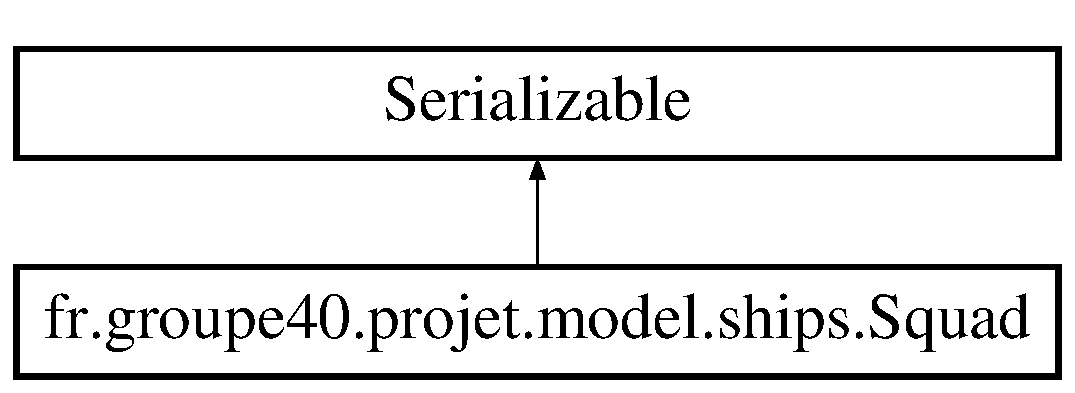
\includegraphics[height=2.000000cm]{classfr_1_1groupe40_1_1projet_1_1model_1_1ships_1_1_squad}
\end{center}
\end{figure}
\subsection*{Public Member Functions}
\begin{DoxyCompactItemize}
\item 
\hyperlink{classfr_1_1groupe40_1_1projet_1_1model_1_1ships_1_1_squad_abf5b8c63d624452536a1fbde111c6424}{Squad} (double percent, \hyperlink{classfr_1_1groupe40_1_1projet_1_1model_1_1planets_1_1_planet}{Planet} src, \hyperlink{classfr_1_1groupe40_1_1projet_1_1model_1_1planets_1_1_planet}{Planet} dest)
\begin{DoxyCompactList}\small\item\em constructor of this squad \end{DoxyCompactList}\item 
\mbox{\Hypertarget{classfr_1_1groupe40_1_1projet_1_1model_1_1ships_1_1_squad_a3f0632de419eece4428900cd090d5ed7}\label{classfr_1_1groupe40_1_1projet_1_1model_1_1ships_1_1_squad_a3f0632de419eece4428900cd090d5ed7}} 
void \hyperlink{classfr_1_1groupe40_1_1projet_1_1model_1_1ships_1_1_squad_a3f0632de419eece4428900cd090d5ed7}{send\+Fleet} ()
\begin{DoxyCompactList}\small\item\em send a fleet, summoned when there s ships that had to be sent \end{DoxyCompactList}\item 
boolean \hyperlink{classfr_1_1groupe40_1_1projet_1_1model_1_1ships_1_1_squad_a16258df054fffdf1acb534665f4d14f4}{squad\+\_\+selected} (double x, double y)
\begin{DoxyCompactList}\small\item\em check if a squad has been selected or not \end{DoxyCompactList}\item 
void \hyperlink{classfr_1_1groupe40_1_1projet_1_1model_1_1ships_1_1_squad_ae4a39cb93983806cdb45e1edee771ecb}{render\+\_\+ships} (Graphics\+Context gc)
\begin{DoxyCompactList}\small\item\em Render every ships of this squad. \end{DoxyCompactList}\item 
void \hyperlink{classfr_1_1groupe40_1_1projet_1_1model_1_1ships_1_1_squad_a3aa04cec78a61156de500c0ffe244745}{update\+\_\+destination} (\hyperlink{classfr_1_1groupe40_1_1projet_1_1model_1_1planets_1_1_planet}{Planet} destination)
\begin{DoxyCompactList}\small\item\em update destination planet of every ships of this squads \end{DoxyCompactList}\item 
\mbox{\Hypertarget{classfr_1_1groupe40_1_1projet_1_1model_1_1ships_1_1_squad_a19aab0462859c2b4d3f3e4f7eba55fb0}\label{classfr_1_1groupe40_1_1projet_1_1model_1_1ships_1_1_squad_a19aab0462859c2b4d3f3e4f7eba55fb0}} 
void \hyperlink{classfr_1_1groupe40_1_1projet_1_1model_1_1ships_1_1_squad_a19aab0462859c2b4d3f3e4f7eba55fb0}{update\+\_\+all\+\_\+positions} (List$<$ \hyperlink{classfr_1_1groupe40_1_1projet_1_1model_1_1planets_1_1_planet}{Planet} $>$ planets)
\begin{DoxyCompactList}\small\item\em Update the position of every ships of this squad. \end{DoxyCompactList}\item 
\mbox{\Hypertarget{classfr_1_1groupe40_1_1projet_1_1model_1_1ships_1_1_squad_ae76aa52a5a5892f28e2b5a89ccc98fa6}\label{classfr_1_1groupe40_1_1projet_1_1model_1_1ships_1_1_squad_ae76aa52a5a5892f28e2b5a89ccc98fa6}} 
void \hyperlink{classfr_1_1groupe40_1_1projet_1_1model_1_1ships_1_1_squad_ae76aa52a5a5892f28e2b5a89ccc98fa6}{update\+Image} ()
\begin{DoxyCompactList}\small\item\em update\+Image of every ships of this squad \end{DoxyCompactList}\item 
void \hyperlink{classfr_1_1groupe40_1_1projet_1_1model_1_1ships_1_1_squad_adaf147d0fd3649c1bf3172c9fd77f096}{update\+\_\+ruler} (\hyperlink{classfr_1_1groupe40_1_1projet_1_1client_1_1_user}{User} ruler)
\begin{DoxyCompactList}\small\item\em update ruler of every ships of this squads \end{DoxyCompactList}\item 
Array\+List$<$ \hyperlink{classfr_1_1groupe40_1_1projet_1_1model_1_1ships_1_1_ship}{Ship} $>$ \hyperlink{classfr_1_1groupe40_1_1projet_1_1model_1_1ships_1_1_squad_a1f5eb0f3d75a52d9f9aeb356eedf603f}{get\+Ships} ()
\item 
void \hyperlink{classfr_1_1groupe40_1_1projet_1_1model_1_1ships_1_1_squad_ab3984439f95320352b71008c4fecce60}{set\+Ships} (Array\+List$<$ \hyperlink{classfr_1_1groupe40_1_1projet_1_1model_1_1ships_1_1_ship}{Ship} $>$ ships)
\item 
int \hyperlink{classfr_1_1groupe40_1_1projet_1_1model_1_1ships_1_1_squad_a7f03812afcb6e3af4cfd589d2557d0ee}{get\+Nb\+\_\+ship} ()
\item 
void \hyperlink{classfr_1_1groupe40_1_1projet_1_1model_1_1ships_1_1_squad_a29e74f6cf438ed28a58fdab135d978e3}{set\+Nb\+\_\+ship} (int nb\+\_\+ship)
\item 
\hyperlink{classfr_1_1groupe40_1_1projet_1_1model_1_1planets_1_1_planet}{Planet} \hyperlink{classfr_1_1groupe40_1_1projet_1_1model_1_1ships_1_1_squad_a12e9417052015e2c3044096372cadc2f}{get\+Source} ()
\item 
void \hyperlink{classfr_1_1groupe40_1_1projet_1_1model_1_1ships_1_1_squad_a748fbe03fce93a59390d5d61b663de53}{set\+Source} (\hyperlink{classfr_1_1groupe40_1_1projet_1_1model_1_1planets_1_1_planet}{Planet} source)
\item 
\hyperlink{classfr_1_1groupe40_1_1projet_1_1model_1_1planets_1_1_planet}{Planet} \hyperlink{classfr_1_1groupe40_1_1projet_1_1model_1_1ships_1_1_squad_a0549670e981d1ed577dec3e84045b00d}{get\+Destination} ()
\item 
void \hyperlink{classfr_1_1groupe40_1_1projet_1_1model_1_1ships_1_1_squad_a7d622ac0b8ba3ec378ca5dd47c7b6dbb}{set\+Destination} (\hyperlink{classfr_1_1groupe40_1_1projet_1_1model_1_1planets_1_1_planet}{Planet} destination)
\item 
int \hyperlink{classfr_1_1groupe40_1_1projet_1_1model_1_1ships_1_1_squad_a7cffe0e2640eae0fff70b9b5b43988e7}{get\+SummonX} ()
\item 
void \hyperlink{classfr_1_1groupe40_1_1projet_1_1model_1_1ships_1_1_squad_a955c5bdf17a95f1dd4a4475bc7426064}{set\+SummonX} (int summonX)
\item 
int \hyperlink{classfr_1_1groupe40_1_1projet_1_1model_1_1ships_1_1_squad_a1957d0d7169c10681d14ade61d8d54ac}{get\+SummonY} ()
\item 
void \hyperlink{classfr_1_1groupe40_1_1projet_1_1model_1_1ships_1_1_squad_a01a24bb024e2c708d192d07f7d89b118}{set\+SummonY} (int summonY)
\item 
boolean \hyperlink{classfr_1_1groupe40_1_1projet_1_1model_1_1ships_1_1_squad_a01723d42948743eb312fdd8ee95eb98d}{is\+Summoning} ()
\item 
void \hyperlink{classfr_1_1groupe40_1_1projet_1_1model_1_1ships_1_1_squad_a5be215f7c74369e01957d51ca5b1e89c}{set\+Summoning} (boolean summoning)
\item 
\mbox{\Hypertarget{classfr_1_1groupe40_1_1projet_1_1model_1_1ships_1_1_squad_a38e7cd0ba4ab8456d9773028cbdad254}\label{classfr_1_1groupe40_1_1projet_1_1model_1_1ships_1_1_squad_a38e7cd0ba4ab8456d9773028cbdad254}} 
\hyperlink{classfr_1_1groupe40_1_1projet_1_1client_1_1_user}{User} {\bfseries get\+Ruler} ()
\end{DoxyCompactItemize}


\subsection{Detailed Description}
\hyperlink{classfr_1_1groupe40_1_1projet_1_1model_1_1ships_1_1_squad}{Squad} object. 

\begin{DoxyAuthor}{Author}
Jordane Masson 

Sarah Portejoie 
\end{DoxyAuthor}


\subsection{Constructor \& Destructor Documentation}
\mbox{\Hypertarget{classfr_1_1groupe40_1_1projet_1_1model_1_1ships_1_1_squad_abf5b8c63d624452536a1fbde111c6424}\label{classfr_1_1groupe40_1_1projet_1_1model_1_1ships_1_1_squad_abf5b8c63d624452536a1fbde111c6424}} 
\index{fr\+::groupe40\+::projet\+::model\+::ships\+::\+Squad@{fr\+::groupe40\+::projet\+::model\+::ships\+::\+Squad}!Squad@{Squad}}
\index{Squad@{Squad}!fr\+::groupe40\+::projet\+::model\+::ships\+::\+Squad@{fr\+::groupe40\+::projet\+::model\+::ships\+::\+Squad}}
\subsubsection{\texorpdfstring{Squad()}{Squad()}}
{\footnotesize\ttfamily fr.\+groupe40.\+projet.\+model.\+ships.\+Squad.\+Squad (\begin{DoxyParamCaption}\item[{double}]{percent,  }\item[{\hyperlink{classfr_1_1groupe40_1_1projet_1_1model_1_1planets_1_1_planet}{Planet}}]{src,  }\item[{\hyperlink{classfr_1_1groupe40_1_1projet_1_1model_1_1planets_1_1_planet}{Planet}}]{dest }\end{DoxyParamCaption})}



constructor of this squad 


\begin{DoxyParams}{Parameters}
{\em percent} & the percent of troups from a planet to send \\
\hline
{\em src} & source planet \\
\hline
{\em dest} & destination planet \\
\hline
\end{DoxyParams}


\subsection{Member Function Documentation}
\mbox{\Hypertarget{classfr_1_1groupe40_1_1projet_1_1model_1_1ships_1_1_squad_a0549670e981d1ed577dec3e84045b00d}\label{classfr_1_1groupe40_1_1projet_1_1model_1_1ships_1_1_squad_a0549670e981d1ed577dec3e84045b00d}} 
\index{fr\+::groupe40\+::projet\+::model\+::ships\+::\+Squad@{fr\+::groupe40\+::projet\+::model\+::ships\+::\+Squad}!get\+Destination@{get\+Destination}}
\index{get\+Destination@{get\+Destination}!fr\+::groupe40\+::projet\+::model\+::ships\+::\+Squad@{fr\+::groupe40\+::projet\+::model\+::ships\+::\+Squad}}
\subsubsection{\texorpdfstring{get\+Destination()}{getDestination()}}
{\footnotesize\ttfamily \hyperlink{classfr_1_1groupe40_1_1projet_1_1model_1_1planets_1_1_planet}{Planet} fr.\+groupe40.\+projet.\+model.\+ships.\+Squad.\+get\+Destination (\begin{DoxyParamCaption}{ }\end{DoxyParamCaption})}

\begin{DoxyReturn}{Returns}
the destination 
\end{DoxyReturn}
\mbox{\Hypertarget{classfr_1_1groupe40_1_1projet_1_1model_1_1ships_1_1_squad_a7f03812afcb6e3af4cfd589d2557d0ee}\label{classfr_1_1groupe40_1_1projet_1_1model_1_1ships_1_1_squad_a7f03812afcb6e3af4cfd589d2557d0ee}} 
\index{fr\+::groupe40\+::projet\+::model\+::ships\+::\+Squad@{fr\+::groupe40\+::projet\+::model\+::ships\+::\+Squad}!get\+Nb\+\_\+ship@{get\+Nb\+\_\+ship}}
\index{get\+Nb\+\_\+ship@{get\+Nb\+\_\+ship}!fr\+::groupe40\+::projet\+::model\+::ships\+::\+Squad@{fr\+::groupe40\+::projet\+::model\+::ships\+::\+Squad}}
\subsubsection{\texorpdfstring{get\+Nb\+\_\+ship()}{getNb\_ship()}}
{\footnotesize\ttfamily int fr.\+groupe40.\+projet.\+model.\+ships.\+Squad.\+get\+Nb\+\_\+ship (\begin{DoxyParamCaption}{ }\end{DoxyParamCaption})}

\begin{DoxyReturn}{Returns}
the nb\+\_\+ship 
\end{DoxyReturn}
\mbox{\Hypertarget{classfr_1_1groupe40_1_1projet_1_1model_1_1ships_1_1_squad_a1f5eb0f3d75a52d9f9aeb356eedf603f}\label{classfr_1_1groupe40_1_1projet_1_1model_1_1ships_1_1_squad_a1f5eb0f3d75a52d9f9aeb356eedf603f}} 
\index{fr\+::groupe40\+::projet\+::model\+::ships\+::\+Squad@{fr\+::groupe40\+::projet\+::model\+::ships\+::\+Squad}!get\+Ships@{get\+Ships}}
\index{get\+Ships@{get\+Ships}!fr\+::groupe40\+::projet\+::model\+::ships\+::\+Squad@{fr\+::groupe40\+::projet\+::model\+::ships\+::\+Squad}}
\subsubsection{\texorpdfstring{get\+Ships()}{getShips()}}
{\footnotesize\ttfamily Array\+List$<$\hyperlink{classfr_1_1groupe40_1_1projet_1_1model_1_1ships_1_1_ship}{Ship}$>$ fr.\+groupe40.\+projet.\+model.\+ships.\+Squad.\+get\+Ships (\begin{DoxyParamCaption}{ }\end{DoxyParamCaption})}

\begin{DoxyReturn}{Returns}
the ships 
\end{DoxyReturn}
\mbox{\Hypertarget{classfr_1_1groupe40_1_1projet_1_1model_1_1ships_1_1_squad_a12e9417052015e2c3044096372cadc2f}\label{classfr_1_1groupe40_1_1projet_1_1model_1_1ships_1_1_squad_a12e9417052015e2c3044096372cadc2f}} 
\index{fr\+::groupe40\+::projet\+::model\+::ships\+::\+Squad@{fr\+::groupe40\+::projet\+::model\+::ships\+::\+Squad}!get\+Source@{get\+Source}}
\index{get\+Source@{get\+Source}!fr\+::groupe40\+::projet\+::model\+::ships\+::\+Squad@{fr\+::groupe40\+::projet\+::model\+::ships\+::\+Squad}}
\subsubsection{\texorpdfstring{get\+Source()}{getSource()}}
{\footnotesize\ttfamily \hyperlink{classfr_1_1groupe40_1_1projet_1_1model_1_1planets_1_1_planet}{Planet} fr.\+groupe40.\+projet.\+model.\+ships.\+Squad.\+get\+Source (\begin{DoxyParamCaption}{ }\end{DoxyParamCaption})}

\begin{DoxyReturn}{Returns}
the source 
\end{DoxyReturn}
\mbox{\Hypertarget{classfr_1_1groupe40_1_1projet_1_1model_1_1ships_1_1_squad_a7cffe0e2640eae0fff70b9b5b43988e7}\label{classfr_1_1groupe40_1_1projet_1_1model_1_1ships_1_1_squad_a7cffe0e2640eae0fff70b9b5b43988e7}} 
\index{fr\+::groupe40\+::projet\+::model\+::ships\+::\+Squad@{fr\+::groupe40\+::projet\+::model\+::ships\+::\+Squad}!get\+SummonX@{get\+SummonX}}
\index{get\+SummonX@{get\+SummonX}!fr\+::groupe40\+::projet\+::model\+::ships\+::\+Squad@{fr\+::groupe40\+::projet\+::model\+::ships\+::\+Squad}}
\subsubsection{\texorpdfstring{get\+Summon\+X()}{getSummonX()}}
{\footnotesize\ttfamily int fr.\+groupe40.\+projet.\+model.\+ships.\+Squad.\+get\+SummonX (\begin{DoxyParamCaption}{ }\end{DoxyParamCaption})}

\begin{DoxyReturn}{Returns}
the summonX 
\end{DoxyReturn}
\mbox{\Hypertarget{classfr_1_1groupe40_1_1projet_1_1model_1_1ships_1_1_squad_a1957d0d7169c10681d14ade61d8d54ac}\label{classfr_1_1groupe40_1_1projet_1_1model_1_1ships_1_1_squad_a1957d0d7169c10681d14ade61d8d54ac}} 
\index{fr\+::groupe40\+::projet\+::model\+::ships\+::\+Squad@{fr\+::groupe40\+::projet\+::model\+::ships\+::\+Squad}!get\+SummonY@{get\+SummonY}}
\index{get\+SummonY@{get\+SummonY}!fr\+::groupe40\+::projet\+::model\+::ships\+::\+Squad@{fr\+::groupe40\+::projet\+::model\+::ships\+::\+Squad}}
\subsubsection{\texorpdfstring{get\+Summon\+Y()}{getSummonY()}}
{\footnotesize\ttfamily int fr.\+groupe40.\+projet.\+model.\+ships.\+Squad.\+get\+SummonY (\begin{DoxyParamCaption}{ }\end{DoxyParamCaption})}

\begin{DoxyReturn}{Returns}
the summonY 
\end{DoxyReturn}
\mbox{\Hypertarget{classfr_1_1groupe40_1_1projet_1_1model_1_1ships_1_1_squad_a01723d42948743eb312fdd8ee95eb98d}\label{classfr_1_1groupe40_1_1projet_1_1model_1_1ships_1_1_squad_a01723d42948743eb312fdd8ee95eb98d}} 
\index{fr\+::groupe40\+::projet\+::model\+::ships\+::\+Squad@{fr\+::groupe40\+::projet\+::model\+::ships\+::\+Squad}!is\+Summoning@{is\+Summoning}}
\index{is\+Summoning@{is\+Summoning}!fr\+::groupe40\+::projet\+::model\+::ships\+::\+Squad@{fr\+::groupe40\+::projet\+::model\+::ships\+::\+Squad}}
\subsubsection{\texorpdfstring{is\+Summoning()}{isSummoning()}}
{\footnotesize\ttfamily boolean fr.\+groupe40.\+projet.\+model.\+ships.\+Squad.\+is\+Summoning (\begin{DoxyParamCaption}{ }\end{DoxyParamCaption})}

\begin{DoxyReturn}{Returns}
the summoning 
\end{DoxyReturn}
\mbox{\Hypertarget{classfr_1_1groupe40_1_1projet_1_1model_1_1ships_1_1_squad_ae4a39cb93983806cdb45e1edee771ecb}\label{classfr_1_1groupe40_1_1projet_1_1model_1_1ships_1_1_squad_ae4a39cb93983806cdb45e1edee771ecb}} 
\index{fr\+::groupe40\+::projet\+::model\+::ships\+::\+Squad@{fr\+::groupe40\+::projet\+::model\+::ships\+::\+Squad}!render\+\_\+ships@{render\+\_\+ships}}
\index{render\+\_\+ships@{render\+\_\+ships}!fr\+::groupe40\+::projet\+::model\+::ships\+::\+Squad@{fr\+::groupe40\+::projet\+::model\+::ships\+::\+Squad}}
\subsubsection{\texorpdfstring{render\+\_\+ships()}{render\_ships()}}
{\footnotesize\ttfamily void fr.\+groupe40.\+projet.\+model.\+ships.\+Squad.\+render\+\_\+ships (\begin{DoxyParamCaption}\item[{Graphics\+Context}]{gc }\end{DoxyParamCaption})}



Render every ships of this squad. 


\begin{DoxyParams}{Parameters}
{\em gc} & Graphics\+Context \\
\hline
\end{DoxyParams}
\mbox{\Hypertarget{classfr_1_1groupe40_1_1projet_1_1model_1_1ships_1_1_squad_a7d622ac0b8ba3ec378ca5dd47c7b6dbb}\label{classfr_1_1groupe40_1_1projet_1_1model_1_1ships_1_1_squad_a7d622ac0b8ba3ec378ca5dd47c7b6dbb}} 
\index{fr\+::groupe40\+::projet\+::model\+::ships\+::\+Squad@{fr\+::groupe40\+::projet\+::model\+::ships\+::\+Squad}!set\+Destination@{set\+Destination}}
\index{set\+Destination@{set\+Destination}!fr\+::groupe40\+::projet\+::model\+::ships\+::\+Squad@{fr\+::groupe40\+::projet\+::model\+::ships\+::\+Squad}}
\subsubsection{\texorpdfstring{set\+Destination()}{setDestination()}}
{\footnotesize\ttfamily void fr.\+groupe40.\+projet.\+model.\+ships.\+Squad.\+set\+Destination (\begin{DoxyParamCaption}\item[{\hyperlink{classfr_1_1groupe40_1_1projet_1_1model_1_1planets_1_1_planet}{Planet}}]{destination }\end{DoxyParamCaption})}


\begin{DoxyParams}{Parameters}
{\em destination} & the destination to set \\
\hline
\end{DoxyParams}
\mbox{\Hypertarget{classfr_1_1groupe40_1_1projet_1_1model_1_1ships_1_1_squad_a29e74f6cf438ed28a58fdab135d978e3}\label{classfr_1_1groupe40_1_1projet_1_1model_1_1ships_1_1_squad_a29e74f6cf438ed28a58fdab135d978e3}} 
\index{fr\+::groupe40\+::projet\+::model\+::ships\+::\+Squad@{fr\+::groupe40\+::projet\+::model\+::ships\+::\+Squad}!set\+Nb\+\_\+ship@{set\+Nb\+\_\+ship}}
\index{set\+Nb\+\_\+ship@{set\+Nb\+\_\+ship}!fr\+::groupe40\+::projet\+::model\+::ships\+::\+Squad@{fr\+::groupe40\+::projet\+::model\+::ships\+::\+Squad}}
\subsubsection{\texorpdfstring{set\+Nb\+\_\+ship()}{setNb\_ship()}}
{\footnotesize\ttfamily void fr.\+groupe40.\+projet.\+model.\+ships.\+Squad.\+set\+Nb\+\_\+ship (\begin{DoxyParamCaption}\item[{int}]{nb\+\_\+ship }\end{DoxyParamCaption})}


\begin{DoxyParams}{Parameters}
{\em nb\+\_\+ship} & the nb\+\_\+ship to set \\
\hline
\end{DoxyParams}
\mbox{\Hypertarget{classfr_1_1groupe40_1_1projet_1_1model_1_1ships_1_1_squad_ab3984439f95320352b71008c4fecce60}\label{classfr_1_1groupe40_1_1projet_1_1model_1_1ships_1_1_squad_ab3984439f95320352b71008c4fecce60}} 
\index{fr\+::groupe40\+::projet\+::model\+::ships\+::\+Squad@{fr\+::groupe40\+::projet\+::model\+::ships\+::\+Squad}!set\+Ships@{set\+Ships}}
\index{set\+Ships@{set\+Ships}!fr\+::groupe40\+::projet\+::model\+::ships\+::\+Squad@{fr\+::groupe40\+::projet\+::model\+::ships\+::\+Squad}}
\subsubsection{\texorpdfstring{set\+Ships()}{setShips()}}
{\footnotesize\ttfamily void fr.\+groupe40.\+projet.\+model.\+ships.\+Squad.\+set\+Ships (\begin{DoxyParamCaption}\item[{Array\+List$<$ \hyperlink{classfr_1_1groupe40_1_1projet_1_1model_1_1ships_1_1_ship}{Ship} $>$}]{ships }\end{DoxyParamCaption})}


\begin{DoxyParams}{Parameters}
{\em ships} & the ships to set \\
\hline
\end{DoxyParams}
\mbox{\Hypertarget{classfr_1_1groupe40_1_1projet_1_1model_1_1ships_1_1_squad_a748fbe03fce93a59390d5d61b663de53}\label{classfr_1_1groupe40_1_1projet_1_1model_1_1ships_1_1_squad_a748fbe03fce93a59390d5d61b663de53}} 
\index{fr\+::groupe40\+::projet\+::model\+::ships\+::\+Squad@{fr\+::groupe40\+::projet\+::model\+::ships\+::\+Squad}!set\+Source@{set\+Source}}
\index{set\+Source@{set\+Source}!fr\+::groupe40\+::projet\+::model\+::ships\+::\+Squad@{fr\+::groupe40\+::projet\+::model\+::ships\+::\+Squad}}
\subsubsection{\texorpdfstring{set\+Source()}{setSource()}}
{\footnotesize\ttfamily void fr.\+groupe40.\+projet.\+model.\+ships.\+Squad.\+set\+Source (\begin{DoxyParamCaption}\item[{\hyperlink{classfr_1_1groupe40_1_1projet_1_1model_1_1planets_1_1_planet}{Planet}}]{source }\end{DoxyParamCaption})}


\begin{DoxyParams}{Parameters}
{\em source} & the source to set \\
\hline
\end{DoxyParams}
\mbox{\Hypertarget{classfr_1_1groupe40_1_1projet_1_1model_1_1ships_1_1_squad_a5be215f7c74369e01957d51ca5b1e89c}\label{classfr_1_1groupe40_1_1projet_1_1model_1_1ships_1_1_squad_a5be215f7c74369e01957d51ca5b1e89c}} 
\index{fr\+::groupe40\+::projet\+::model\+::ships\+::\+Squad@{fr\+::groupe40\+::projet\+::model\+::ships\+::\+Squad}!set\+Summoning@{set\+Summoning}}
\index{set\+Summoning@{set\+Summoning}!fr\+::groupe40\+::projet\+::model\+::ships\+::\+Squad@{fr\+::groupe40\+::projet\+::model\+::ships\+::\+Squad}}
\subsubsection{\texorpdfstring{set\+Summoning()}{setSummoning()}}
{\footnotesize\ttfamily void fr.\+groupe40.\+projet.\+model.\+ships.\+Squad.\+set\+Summoning (\begin{DoxyParamCaption}\item[{boolean}]{summoning }\end{DoxyParamCaption})}


\begin{DoxyParams}{Parameters}
{\em summoning} & the summoning to set \\
\hline
\end{DoxyParams}
\mbox{\Hypertarget{classfr_1_1groupe40_1_1projet_1_1model_1_1ships_1_1_squad_a955c5bdf17a95f1dd4a4475bc7426064}\label{classfr_1_1groupe40_1_1projet_1_1model_1_1ships_1_1_squad_a955c5bdf17a95f1dd4a4475bc7426064}} 
\index{fr\+::groupe40\+::projet\+::model\+::ships\+::\+Squad@{fr\+::groupe40\+::projet\+::model\+::ships\+::\+Squad}!set\+SummonX@{set\+SummonX}}
\index{set\+SummonX@{set\+SummonX}!fr\+::groupe40\+::projet\+::model\+::ships\+::\+Squad@{fr\+::groupe40\+::projet\+::model\+::ships\+::\+Squad}}
\subsubsection{\texorpdfstring{set\+Summon\+X()}{setSummonX()}}
{\footnotesize\ttfamily void fr.\+groupe40.\+projet.\+model.\+ships.\+Squad.\+set\+SummonX (\begin{DoxyParamCaption}\item[{int}]{summonX }\end{DoxyParamCaption})}


\begin{DoxyParams}{Parameters}
{\em summonX} & the summonX to set \\
\hline
\end{DoxyParams}
\mbox{\Hypertarget{classfr_1_1groupe40_1_1projet_1_1model_1_1ships_1_1_squad_a01a24bb024e2c708d192d07f7d89b118}\label{classfr_1_1groupe40_1_1projet_1_1model_1_1ships_1_1_squad_a01a24bb024e2c708d192d07f7d89b118}} 
\index{fr\+::groupe40\+::projet\+::model\+::ships\+::\+Squad@{fr\+::groupe40\+::projet\+::model\+::ships\+::\+Squad}!set\+SummonY@{set\+SummonY}}
\index{set\+SummonY@{set\+SummonY}!fr\+::groupe40\+::projet\+::model\+::ships\+::\+Squad@{fr\+::groupe40\+::projet\+::model\+::ships\+::\+Squad}}
\subsubsection{\texorpdfstring{set\+Summon\+Y()}{setSummonY()}}
{\footnotesize\ttfamily void fr.\+groupe40.\+projet.\+model.\+ships.\+Squad.\+set\+SummonY (\begin{DoxyParamCaption}\item[{int}]{summonY }\end{DoxyParamCaption})}


\begin{DoxyParams}{Parameters}
{\em summonY} & the summonY to set \\
\hline
\end{DoxyParams}
\mbox{\Hypertarget{classfr_1_1groupe40_1_1projet_1_1model_1_1ships_1_1_squad_a16258df054fffdf1acb534665f4d14f4}\label{classfr_1_1groupe40_1_1projet_1_1model_1_1ships_1_1_squad_a16258df054fffdf1acb534665f4d14f4}} 
\index{fr\+::groupe40\+::projet\+::model\+::ships\+::\+Squad@{fr\+::groupe40\+::projet\+::model\+::ships\+::\+Squad}!squad\+\_\+selected@{squad\+\_\+selected}}
\index{squad\+\_\+selected@{squad\+\_\+selected}!fr\+::groupe40\+::projet\+::model\+::ships\+::\+Squad@{fr\+::groupe40\+::projet\+::model\+::ships\+::\+Squad}}
\subsubsection{\texorpdfstring{squad\+\_\+selected()}{squad\_selected()}}
{\footnotesize\ttfamily boolean fr.\+groupe40.\+projet.\+model.\+ships.\+Squad.\+squad\+\_\+selected (\begin{DoxyParamCaption}\item[{double}]{x,  }\item[{double}]{y }\end{DoxyParamCaption})}



check if a squad has been selected or not 


\begin{DoxyParams}{Parameters}
{\em x} & position to check \\
\hline
{\em y} & position to check \\
\hline
\end{DoxyParams}
\begin{DoxyReturn}{Returns}
true if a squad has been selected 
\end{DoxyReturn}
\mbox{\Hypertarget{classfr_1_1groupe40_1_1projet_1_1model_1_1ships_1_1_squad_a3aa04cec78a61156de500c0ffe244745}\label{classfr_1_1groupe40_1_1projet_1_1model_1_1ships_1_1_squad_a3aa04cec78a61156de500c0ffe244745}} 
\index{fr\+::groupe40\+::projet\+::model\+::ships\+::\+Squad@{fr\+::groupe40\+::projet\+::model\+::ships\+::\+Squad}!update\+\_\+destination@{update\+\_\+destination}}
\index{update\+\_\+destination@{update\+\_\+destination}!fr\+::groupe40\+::projet\+::model\+::ships\+::\+Squad@{fr\+::groupe40\+::projet\+::model\+::ships\+::\+Squad}}
\subsubsection{\texorpdfstring{update\+\_\+destination()}{update\_destination()}}
{\footnotesize\ttfamily void fr.\+groupe40.\+projet.\+model.\+ships.\+Squad.\+update\+\_\+destination (\begin{DoxyParamCaption}\item[{\hyperlink{classfr_1_1groupe40_1_1projet_1_1model_1_1planets_1_1_planet}{Planet}}]{destination }\end{DoxyParamCaption})}



update destination planet of every ships of this squads 


\begin{DoxyParams}{Parameters}
{\em destination} & the new destination \\
\hline
\end{DoxyParams}
\mbox{\Hypertarget{classfr_1_1groupe40_1_1projet_1_1model_1_1ships_1_1_squad_adaf147d0fd3649c1bf3172c9fd77f096}\label{classfr_1_1groupe40_1_1projet_1_1model_1_1ships_1_1_squad_adaf147d0fd3649c1bf3172c9fd77f096}} 
\index{fr\+::groupe40\+::projet\+::model\+::ships\+::\+Squad@{fr\+::groupe40\+::projet\+::model\+::ships\+::\+Squad}!update\+\_\+ruler@{update\+\_\+ruler}}
\index{update\+\_\+ruler@{update\+\_\+ruler}!fr\+::groupe40\+::projet\+::model\+::ships\+::\+Squad@{fr\+::groupe40\+::projet\+::model\+::ships\+::\+Squad}}
\subsubsection{\texorpdfstring{update\+\_\+ruler()}{update\_ruler()}}
{\footnotesize\ttfamily void fr.\+groupe40.\+projet.\+model.\+ships.\+Squad.\+update\+\_\+ruler (\begin{DoxyParamCaption}\item[{\hyperlink{classfr_1_1groupe40_1_1projet_1_1client_1_1_user}{User}}]{ruler }\end{DoxyParamCaption})}



update ruler of every ships of this squads 


\begin{DoxyParams}{Parameters}
{\em ruler} & the new ruler \\
\hline
\end{DoxyParams}


The documentation for this class was generated from the following file\+:\begin{DoxyCompactItemize}
\item 
src/fr/groupe40/projet/model/ships/Squad.\+java\end{DoxyCompactItemize}

\hypertarget{classfr_1_1groupe40_1_1projet_1_1model_1_1planets_1_1_square_planet}{}\section{fr.\+groupe40.\+projet.\+model.\+planets.\+Square\+Planet Class Reference}
\label{classfr_1_1groupe40_1_1projet_1_1model_1_1planets_1_1_square_planet}\index{fr.\+groupe40.\+projet.\+model.\+planets.\+Square\+Planet@{fr.\+groupe40.\+projet.\+model.\+planets.\+Square\+Planet}}


Square planet T\+O\+DO.  


Inheritance diagram for fr.\+groupe40.\+projet.\+model.\+planets.\+Square\+Planet\+:\begin{figure}[H]
\begin{center}
\leavevmode
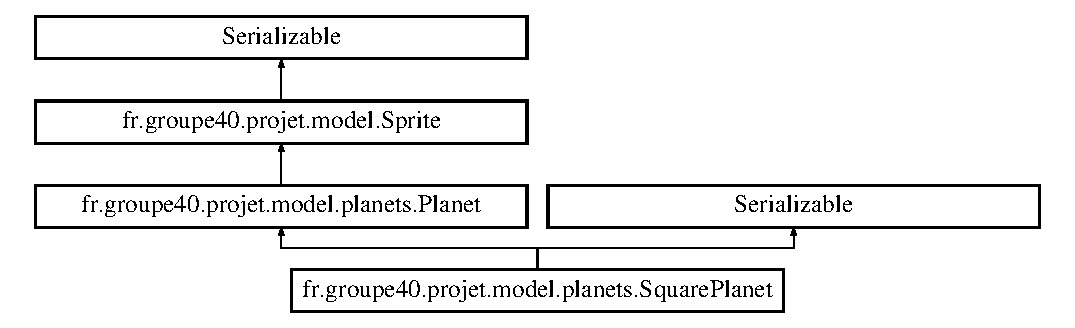
\includegraphics[height=3.957597cm]{classfr_1_1groupe40_1_1projet_1_1model_1_1planets_1_1_square_planet}
\end{center}
\end{figure}
\subsection*{Public Member Functions}
\begin{DoxyCompactItemize}
\item 
\mbox{\Hypertarget{classfr_1_1groupe40_1_1projet_1_1model_1_1planets_1_1_square_planet_af5c59fb2f1bbd57745396640f074f3af}\label{classfr_1_1groupe40_1_1projet_1_1model_1_1planets_1_1_square_planet_af5c59fb2f1bbd57745396640f074f3af}} 
{\bfseries Square\+Planet} (String path, \hyperlink{classfr_1_1groupe40_1_1projet_1_1client_1_1_user}{User} ruler, boolean is\+Planet, int x, int y)
\end{DoxyCompactItemize}


\subsection{Detailed Description}
Square planet T\+O\+DO. 

\begin{DoxyAuthor}{Author}
Jordane Masson 

Sarah Portejoie 
\end{DoxyAuthor}


The documentation for this class was generated from the following file\+:\begin{DoxyCompactItemize}
\item 
src/fr/groupe40/projet/model/planets/Square\+Planet.\+java\end{DoxyCompactItemize}

\hypertarget{classfr_1_1groupe40_1_1projet_1_1client_1_1_user}{}\section{fr.\+groupe40.\+projet.\+client.\+User Class Reference}
\label{classfr_1_1groupe40_1_1projet_1_1client_1_1_user}\index{fr.\+groupe40.\+projet.\+client.\+User@{fr.\+groupe40.\+projet.\+client.\+User}}
Inheritance diagram for fr.\+groupe40.\+projet.\+client.\+User\+:\begin{figure}[H]
\begin{center}
\leavevmode
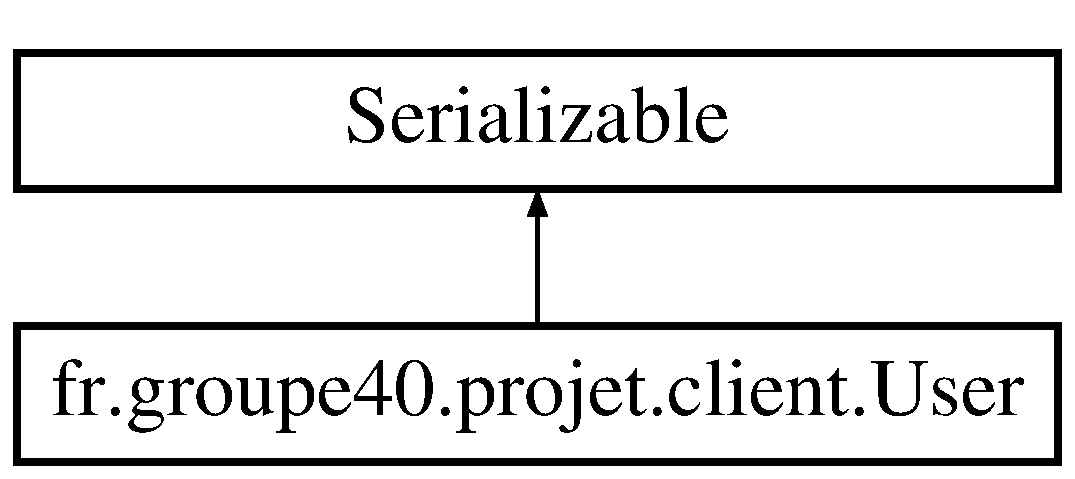
\includegraphics[height=2.000000cm]{classfr_1_1groupe40_1_1projet_1_1client_1_1_user}
\end{center}
\end{figure}
\subsection*{Public Member Functions}
\begin{DoxyCompactItemize}
\item 
\hyperlink{classfr_1_1groupe40_1_1projet_1_1client_1_1_user_acd2d859d7679c886c0445aa8d18f177f}{User} (int faction, int id)
\begin{DoxyCompactList}\small\item\em Create a new user from a faction and an id. \end{DoxyCompactList}\item 
\hyperlink{classfr_1_1groupe40_1_1projet_1_1client_1_1_user_ae3f43ec29e7b599c4f203bc0fa9c5fd5}{User} (int faction)
\begin{DoxyCompactList}\small\item\em Create a user only from his id. \end{DoxyCompactList}\item 
\hyperlink{classfr_1_1groupe40_1_1projet_1_1client_1_1_user_aadb257aeb0ed9544df923a83f8ed1e61}{User} (\hyperlink{classfr_1_1groupe40_1_1projet_1_1client_1_1_user}{User} user)
\begin{DoxyCompactList}\small\item\em create an user from an user \end{DoxyCompactList}\item 
\hyperlink{classfr_1_1groupe40_1_1projet_1_1model_1_1ships_1_1_squad}{Squad} \hyperlink{classfr_1_1groupe40_1_1projet_1_1client_1_1_user_a32007a7692972de524c9a03c813b97d1}{send\+Fleet\+AI} (\hyperlink{classfr_1_1groupe40_1_1projet_1_1model_1_1planets_1_1_planet}{Planet} source, \hyperlink{classfr_1_1groupe40_1_1projet_1_1model_1_1planets_1_1_planet}{Planet} destination)
\begin{DoxyCompactList}\small\item\em send fleet automatization for ai user \end{DoxyCompactList}\item 
int \hyperlink{classfr_1_1groupe40_1_1projet_1_1client_1_1_user_a32446cf36b262fc03f5dc96a207a5375}{get\+Faction} ()
\begin{DoxyCompactList}\small\item\em return the faction of an user \end{DoxyCompactList}\item 
void \hyperlink{classfr_1_1groupe40_1_1projet_1_1client_1_1_user_af10956b4173a0bcd31fe89d450aa1cf1}{set\+Faction} (int faction)
\begin{DoxyCompactList}\small\item\em set the faction of an user \end{DoxyCompactList}\item 
int \hyperlink{classfr_1_1groupe40_1_1projet_1_1client_1_1_user_a43318df463de36284d68071ec0a59f34}{get\+Id} ()
\begin{DoxyCompactList}\small\item\em return the id of an user \end{DoxyCompactList}\item 
void \hyperlink{classfr_1_1groupe40_1_1projet_1_1client_1_1_user_a81fb7ded5bdecebd2ddce5d03999f568}{set\+Id} (int id)
\begin{DoxyCompactList}\small\item\em set a new id for an user \end{DoxyCompactList}\item 
int \hyperlink{classfr_1_1groupe40_1_1projet_1_1client_1_1_user_aa1a898620fe07e7b13579cb9f9e7b865}{get\+Percent\+\_\+of\+\_\+troups\+\_\+to\+\_\+send} ()
\item 
void \hyperlink{classfr_1_1groupe40_1_1projet_1_1client_1_1_user_adcf16120e83f73eb8ac0be34fce57b7b}{set\+Percent\+\_\+of\+\_\+troups\+\_\+to\+\_\+send} (int percent\+\_\+of\+\_\+troups\+\_\+to\+\_\+send)
\item 
\hyperlink{classfr_1_1groupe40_1_1projet_1_1model_1_1planets_1_1_planet}{Planet} \hyperlink{classfr_1_1groupe40_1_1projet_1_1client_1_1_user_a1a8f8f74a34b5e4745f23089a223f6d6}{get\+Destination} ()
\item 
void \hyperlink{classfr_1_1groupe40_1_1projet_1_1client_1_1_user_a4b36462569cbce5ac7c47ea1394f9a4c}{set\+Destination} (\hyperlink{classfr_1_1groupe40_1_1projet_1_1model_1_1planets_1_1_planet}{Planet} destination)
\item 
\hyperlink{classfr_1_1groupe40_1_1projet_1_1model_1_1planets_1_1_planet}{Planet} \hyperlink{classfr_1_1groupe40_1_1projet_1_1client_1_1_user_a8d5a9ada62388f690f9dd9d70d4f4d1c}{get\+Source} ()
\item 
void \hyperlink{classfr_1_1groupe40_1_1projet_1_1client_1_1_user_a3da3fb9206c4e00df7700940bd69f601}{set\+Source} (\hyperlink{classfr_1_1groupe40_1_1projet_1_1model_1_1planets_1_1_planet}{Planet} source)
\item 
boolean \hyperlink{classfr_1_1groupe40_1_1projet_1_1client_1_1_user_a0e846e067a87f2cedcc43f25968f000f}{is\+Lost} ()
\begin{DoxyCompactList}\small\item\em return if this user has lost or not \end{DoxyCompactList}\item 
void \hyperlink{classfr_1_1groupe40_1_1projet_1_1client_1_1_user_af0d8095643e7901ef0320d4245da0771}{set\+Lost} (boolean lost)
\begin{DoxyCompactList}\small\item\em set the lost state of an user \end{DoxyCompactList}\item 
boolean \hyperlink{classfr_1_1groupe40_1_1projet_1_1client_1_1_user_a9ef8e41efa22dad7be2e4b9966ff7818}{equals} (\hyperlink{classfr_1_1groupe40_1_1projet_1_1client_1_1_user}{User} u)
\begin{DoxyCompactList}\small\item\em compare two user \end{DoxyCompactList}\end{DoxyCompactItemize}


\subsection{Detailed Description}
\begin{DoxyAuthor}{Author}
Jordane Masson 

Sarah Portejoie 
\end{DoxyAuthor}


\subsection{Constructor \& Destructor Documentation}
\mbox{\Hypertarget{classfr_1_1groupe40_1_1projet_1_1client_1_1_user_acd2d859d7679c886c0445aa8d18f177f}\label{classfr_1_1groupe40_1_1projet_1_1client_1_1_user_acd2d859d7679c886c0445aa8d18f177f}} 
\index{fr\+::groupe40\+::projet\+::client\+::\+User@{fr\+::groupe40\+::projet\+::client\+::\+User}!User@{User}}
\index{User@{User}!fr\+::groupe40\+::projet\+::client\+::\+User@{fr\+::groupe40\+::projet\+::client\+::\+User}}
\subsubsection{\texorpdfstring{User()}{User()}\hspace{0.1cm}{\footnotesize\ttfamily [1/3]}}
{\footnotesize\ttfamily fr.\+groupe40.\+projet.\+client.\+User.\+User (\begin{DoxyParamCaption}\item[{int}]{faction,  }\item[{int}]{id }\end{DoxyParamCaption})}



Create a new user from a faction and an id. 


\begin{DoxyParams}{Parameters}
{\em faction} & the faction of this user \\
\hline
{\em id} & the id of this user \\
\hline
\end{DoxyParams}
\mbox{\Hypertarget{classfr_1_1groupe40_1_1projet_1_1client_1_1_user_ae3f43ec29e7b599c4f203bc0fa9c5fd5}\label{classfr_1_1groupe40_1_1projet_1_1client_1_1_user_ae3f43ec29e7b599c4f203bc0fa9c5fd5}} 
\index{fr\+::groupe40\+::projet\+::client\+::\+User@{fr\+::groupe40\+::projet\+::client\+::\+User}!User@{User}}
\index{User@{User}!fr\+::groupe40\+::projet\+::client\+::\+User@{fr\+::groupe40\+::projet\+::client\+::\+User}}
\subsubsection{\texorpdfstring{User()}{User()}\hspace{0.1cm}{\footnotesize\ttfamily [2/3]}}
{\footnotesize\ttfamily fr.\+groupe40.\+projet.\+client.\+User.\+User (\begin{DoxyParamCaption}\item[{int}]{faction }\end{DoxyParamCaption})}



Create a user only from his id. 


\begin{DoxyParams}{Parameters}
{\em faction} & the faction of this player \\
\hline
\end{DoxyParams}
\mbox{\Hypertarget{classfr_1_1groupe40_1_1projet_1_1client_1_1_user_aadb257aeb0ed9544df923a83f8ed1e61}\label{classfr_1_1groupe40_1_1projet_1_1client_1_1_user_aadb257aeb0ed9544df923a83f8ed1e61}} 
\index{fr\+::groupe40\+::projet\+::client\+::\+User@{fr\+::groupe40\+::projet\+::client\+::\+User}!User@{User}}
\index{User@{User}!fr\+::groupe40\+::projet\+::client\+::\+User@{fr\+::groupe40\+::projet\+::client\+::\+User}}
\subsubsection{\texorpdfstring{User()}{User()}\hspace{0.1cm}{\footnotesize\ttfamily [3/3]}}
{\footnotesize\ttfamily fr.\+groupe40.\+projet.\+client.\+User.\+User (\begin{DoxyParamCaption}\item[{\hyperlink{classfr_1_1groupe40_1_1projet_1_1client_1_1_user}{User}}]{user }\end{DoxyParamCaption})}



create an user from an user 


\begin{DoxyParams}{Parameters}
{\em user} & to copy parameters from \\
\hline
\end{DoxyParams}


\subsection{Member Function Documentation}
\mbox{\Hypertarget{classfr_1_1groupe40_1_1projet_1_1client_1_1_user_a9ef8e41efa22dad7be2e4b9966ff7818}\label{classfr_1_1groupe40_1_1projet_1_1client_1_1_user_a9ef8e41efa22dad7be2e4b9966ff7818}} 
\index{fr\+::groupe40\+::projet\+::client\+::\+User@{fr\+::groupe40\+::projet\+::client\+::\+User}!equals@{equals}}
\index{equals@{equals}!fr\+::groupe40\+::projet\+::client\+::\+User@{fr\+::groupe40\+::projet\+::client\+::\+User}}
\subsubsection{\texorpdfstring{equals()}{equals()}}
{\footnotesize\ttfamily boolean fr.\+groupe40.\+projet.\+client.\+User.\+equals (\begin{DoxyParamCaption}\item[{\hyperlink{classfr_1_1groupe40_1_1projet_1_1client_1_1_user}{User}}]{u }\end{DoxyParamCaption})}



compare two user 


\begin{DoxyParams}{Parameters}
{\em u} & \\
\hline
\end{DoxyParams}
\begin{DoxyReturn}{Returns}
true if they\textquotesingle{}re both equals, else false 
\end{DoxyReturn}
\mbox{\Hypertarget{classfr_1_1groupe40_1_1projet_1_1client_1_1_user_a1a8f8f74a34b5e4745f23089a223f6d6}\label{classfr_1_1groupe40_1_1projet_1_1client_1_1_user_a1a8f8f74a34b5e4745f23089a223f6d6}} 
\index{fr\+::groupe40\+::projet\+::client\+::\+User@{fr\+::groupe40\+::projet\+::client\+::\+User}!get\+Destination@{get\+Destination}}
\index{get\+Destination@{get\+Destination}!fr\+::groupe40\+::projet\+::client\+::\+User@{fr\+::groupe40\+::projet\+::client\+::\+User}}
\subsubsection{\texorpdfstring{get\+Destination()}{getDestination()}}
{\footnotesize\ttfamily \hyperlink{classfr_1_1groupe40_1_1projet_1_1model_1_1planets_1_1_planet}{Planet} fr.\+groupe40.\+projet.\+client.\+User.\+get\+Destination (\begin{DoxyParamCaption}{ }\end{DoxyParamCaption})}

\begin{DoxyReturn}{Returns}
the destination 
\end{DoxyReturn}
\mbox{\Hypertarget{classfr_1_1groupe40_1_1projet_1_1client_1_1_user_a32446cf36b262fc03f5dc96a207a5375}\label{classfr_1_1groupe40_1_1projet_1_1client_1_1_user_a32446cf36b262fc03f5dc96a207a5375}} 
\index{fr\+::groupe40\+::projet\+::client\+::\+User@{fr\+::groupe40\+::projet\+::client\+::\+User}!get\+Faction@{get\+Faction}}
\index{get\+Faction@{get\+Faction}!fr\+::groupe40\+::projet\+::client\+::\+User@{fr\+::groupe40\+::projet\+::client\+::\+User}}
\subsubsection{\texorpdfstring{get\+Faction()}{getFaction()}}
{\footnotesize\ttfamily int fr.\+groupe40.\+projet.\+client.\+User.\+get\+Faction (\begin{DoxyParamCaption}{ }\end{DoxyParamCaption})}



return the faction of an user 

\begin{DoxyReturn}{Returns}
faction 
\end{DoxyReturn}
\mbox{\Hypertarget{classfr_1_1groupe40_1_1projet_1_1client_1_1_user_a43318df463de36284d68071ec0a59f34}\label{classfr_1_1groupe40_1_1projet_1_1client_1_1_user_a43318df463de36284d68071ec0a59f34}} 
\index{fr\+::groupe40\+::projet\+::client\+::\+User@{fr\+::groupe40\+::projet\+::client\+::\+User}!get\+Id@{get\+Id}}
\index{get\+Id@{get\+Id}!fr\+::groupe40\+::projet\+::client\+::\+User@{fr\+::groupe40\+::projet\+::client\+::\+User}}
\subsubsection{\texorpdfstring{get\+Id()}{getId()}}
{\footnotesize\ttfamily int fr.\+groupe40.\+projet.\+client.\+User.\+get\+Id (\begin{DoxyParamCaption}{ }\end{DoxyParamCaption})}



return the id of an user 

\begin{DoxyReturn}{Returns}
id 
\end{DoxyReturn}
\mbox{\Hypertarget{classfr_1_1groupe40_1_1projet_1_1client_1_1_user_aa1a898620fe07e7b13579cb9f9e7b865}\label{classfr_1_1groupe40_1_1projet_1_1client_1_1_user_aa1a898620fe07e7b13579cb9f9e7b865}} 
\index{fr\+::groupe40\+::projet\+::client\+::\+User@{fr\+::groupe40\+::projet\+::client\+::\+User}!get\+Percent\+\_\+of\+\_\+troups\+\_\+to\+\_\+send@{get\+Percent\+\_\+of\+\_\+troups\+\_\+to\+\_\+send}}
\index{get\+Percent\+\_\+of\+\_\+troups\+\_\+to\+\_\+send@{get\+Percent\+\_\+of\+\_\+troups\+\_\+to\+\_\+send}!fr\+::groupe40\+::projet\+::client\+::\+User@{fr\+::groupe40\+::projet\+::client\+::\+User}}
\subsubsection{\texorpdfstring{get\+Percent\+\_\+of\+\_\+troups\+\_\+to\+\_\+send()}{getPercent\_of\_troups\_to\_send()}}
{\footnotesize\ttfamily int fr.\+groupe40.\+projet.\+client.\+User.\+get\+Percent\+\_\+of\+\_\+troups\+\_\+to\+\_\+send (\begin{DoxyParamCaption}{ }\end{DoxyParamCaption})}

\begin{DoxyReturn}{Returns}
the percent\+\_\+of\+\_\+troups\+\_\+to\+\_\+send 
\end{DoxyReturn}
\mbox{\Hypertarget{classfr_1_1groupe40_1_1projet_1_1client_1_1_user_a8d5a9ada62388f690f9dd9d70d4f4d1c}\label{classfr_1_1groupe40_1_1projet_1_1client_1_1_user_a8d5a9ada62388f690f9dd9d70d4f4d1c}} 
\index{fr\+::groupe40\+::projet\+::client\+::\+User@{fr\+::groupe40\+::projet\+::client\+::\+User}!get\+Source@{get\+Source}}
\index{get\+Source@{get\+Source}!fr\+::groupe40\+::projet\+::client\+::\+User@{fr\+::groupe40\+::projet\+::client\+::\+User}}
\subsubsection{\texorpdfstring{get\+Source()}{getSource()}}
{\footnotesize\ttfamily \hyperlink{classfr_1_1groupe40_1_1projet_1_1model_1_1planets_1_1_planet}{Planet} fr.\+groupe40.\+projet.\+client.\+User.\+get\+Source (\begin{DoxyParamCaption}{ }\end{DoxyParamCaption})}

\begin{DoxyReturn}{Returns}
the source 
\end{DoxyReturn}
\mbox{\Hypertarget{classfr_1_1groupe40_1_1projet_1_1client_1_1_user_a0e846e067a87f2cedcc43f25968f000f}\label{classfr_1_1groupe40_1_1projet_1_1client_1_1_user_a0e846e067a87f2cedcc43f25968f000f}} 
\index{fr\+::groupe40\+::projet\+::client\+::\+User@{fr\+::groupe40\+::projet\+::client\+::\+User}!is\+Lost@{is\+Lost}}
\index{is\+Lost@{is\+Lost}!fr\+::groupe40\+::projet\+::client\+::\+User@{fr\+::groupe40\+::projet\+::client\+::\+User}}
\subsubsection{\texorpdfstring{is\+Lost()}{isLost()}}
{\footnotesize\ttfamily boolean fr.\+groupe40.\+projet.\+client.\+User.\+is\+Lost (\begin{DoxyParamCaption}{ }\end{DoxyParamCaption})}



return if this user has lost or not 

\begin{DoxyReturn}{Returns}
lost 
\end{DoxyReturn}
\mbox{\Hypertarget{classfr_1_1groupe40_1_1projet_1_1client_1_1_user_a32007a7692972de524c9a03c813b97d1}\label{classfr_1_1groupe40_1_1projet_1_1client_1_1_user_a32007a7692972de524c9a03c813b97d1}} 
\index{fr\+::groupe40\+::projet\+::client\+::\+User@{fr\+::groupe40\+::projet\+::client\+::\+User}!send\+Fleet\+AI@{send\+Fleet\+AI}}
\index{send\+Fleet\+AI@{send\+Fleet\+AI}!fr\+::groupe40\+::projet\+::client\+::\+User@{fr\+::groupe40\+::projet\+::client\+::\+User}}
\subsubsection{\texorpdfstring{send\+Fleet\+A\+I()}{sendFleetAI()}}
{\footnotesize\ttfamily \hyperlink{classfr_1_1groupe40_1_1projet_1_1model_1_1ships_1_1_squad}{Squad} fr.\+groupe40.\+projet.\+client.\+User.\+send\+Fleet\+AI (\begin{DoxyParamCaption}\item[{\hyperlink{classfr_1_1groupe40_1_1projet_1_1model_1_1planets_1_1_planet}{Planet}}]{source,  }\item[{\hyperlink{classfr_1_1groupe40_1_1projet_1_1model_1_1planets_1_1_planet}{Planet}}]{destination }\end{DoxyParamCaption})}



send fleet automatization for ai user 


\begin{DoxyParams}{Parameters}
{\em source} & the source planet \\
\hline
{\em destination} & the destination planet \\
\hline
\end{DoxyParams}
\begin{DoxyReturn}{Returns}
the squad that has been send, else null 
\end{DoxyReturn}
\mbox{\Hypertarget{classfr_1_1groupe40_1_1projet_1_1client_1_1_user_a4b36462569cbce5ac7c47ea1394f9a4c}\label{classfr_1_1groupe40_1_1projet_1_1client_1_1_user_a4b36462569cbce5ac7c47ea1394f9a4c}} 
\index{fr\+::groupe40\+::projet\+::client\+::\+User@{fr\+::groupe40\+::projet\+::client\+::\+User}!set\+Destination@{set\+Destination}}
\index{set\+Destination@{set\+Destination}!fr\+::groupe40\+::projet\+::client\+::\+User@{fr\+::groupe40\+::projet\+::client\+::\+User}}
\subsubsection{\texorpdfstring{set\+Destination()}{setDestination()}}
{\footnotesize\ttfamily void fr.\+groupe40.\+projet.\+client.\+User.\+set\+Destination (\begin{DoxyParamCaption}\item[{\hyperlink{classfr_1_1groupe40_1_1projet_1_1model_1_1planets_1_1_planet}{Planet}}]{destination }\end{DoxyParamCaption})}


\begin{DoxyParams}{Parameters}
{\em destination} & the destination to set \\
\hline
\end{DoxyParams}
\mbox{\Hypertarget{classfr_1_1groupe40_1_1projet_1_1client_1_1_user_af10956b4173a0bcd31fe89d450aa1cf1}\label{classfr_1_1groupe40_1_1projet_1_1client_1_1_user_af10956b4173a0bcd31fe89d450aa1cf1}} 
\index{fr\+::groupe40\+::projet\+::client\+::\+User@{fr\+::groupe40\+::projet\+::client\+::\+User}!set\+Faction@{set\+Faction}}
\index{set\+Faction@{set\+Faction}!fr\+::groupe40\+::projet\+::client\+::\+User@{fr\+::groupe40\+::projet\+::client\+::\+User}}
\subsubsection{\texorpdfstring{set\+Faction()}{setFaction()}}
{\footnotesize\ttfamily void fr.\+groupe40.\+projet.\+client.\+User.\+set\+Faction (\begin{DoxyParamCaption}\item[{int}]{faction }\end{DoxyParamCaption})}



set the faction of an user 


\begin{DoxyParams}{Parameters}
{\em faction} & his new faction \\
\hline
\end{DoxyParams}
\mbox{\Hypertarget{classfr_1_1groupe40_1_1projet_1_1client_1_1_user_a81fb7ded5bdecebd2ddce5d03999f568}\label{classfr_1_1groupe40_1_1projet_1_1client_1_1_user_a81fb7ded5bdecebd2ddce5d03999f568}} 
\index{fr\+::groupe40\+::projet\+::client\+::\+User@{fr\+::groupe40\+::projet\+::client\+::\+User}!set\+Id@{set\+Id}}
\index{set\+Id@{set\+Id}!fr\+::groupe40\+::projet\+::client\+::\+User@{fr\+::groupe40\+::projet\+::client\+::\+User}}
\subsubsection{\texorpdfstring{set\+Id()}{setId()}}
{\footnotesize\ttfamily void fr.\+groupe40.\+projet.\+client.\+User.\+set\+Id (\begin{DoxyParamCaption}\item[{int}]{id }\end{DoxyParamCaption})}



set a new id for an user 


\begin{DoxyParams}{Parameters}
{\em id} & \\
\hline
\end{DoxyParams}
\mbox{\Hypertarget{classfr_1_1groupe40_1_1projet_1_1client_1_1_user_af0d8095643e7901ef0320d4245da0771}\label{classfr_1_1groupe40_1_1projet_1_1client_1_1_user_af0d8095643e7901ef0320d4245da0771}} 
\index{fr\+::groupe40\+::projet\+::client\+::\+User@{fr\+::groupe40\+::projet\+::client\+::\+User}!set\+Lost@{set\+Lost}}
\index{set\+Lost@{set\+Lost}!fr\+::groupe40\+::projet\+::client\+::\+User@{fr\+::groupe40\+::projet\+::client\+::\+User}}
\subsubsection{\texorpdfstring{set\+Lost()}{setLost()}}
{\footnotesize\ttfamily void fr.\+groupe40.\+projet.\+client.\+User.\+set\+Lost (\begin{DoxyParamCaption}\item[{boolean}]{lost }\end{DoxyParamCaption})}



set the lost state of an user 


\begin{DoxyParams}{Parameters}
{\em lost} & \\
\hline
\end{DoxyParams}
\mbox{\Hypertarget{classfr_1_1groupe40_1_1projet_1_1client_1_1_user_adcf16120e83f73eb8ac0be34fce57b7b}\label{classfr_1_1groupe40_1_1projet_1_1client_1_1_user_adcf16120e83f73eb8ac0be34fce57b7b}} 
\index{fr\+::groupe40\+::projet\+::client\+::\+User@{fr\+::groupe40\+::projet\+::client\+::\+User}!set\+Percent\+\_\+of\+\_\+troups\+\_\+to\+\_\+send@{set\+Percent\+\_\+of\+\_\+troups\+\_\+to\+\_\+send}}
\index{set\+Percent\+\_\+of\+\_\+troups\+\_\+to\+\_\+send@{set\+Percent\+\_\+of\+\_\+troups\+\_\+to\+\_\+send}!fr\+::groupe40\+::projet\+::client\+::\+User@{fr\+::groupe40\+::projet\+::client\+::\+User}}
\subsubsection{\texorpdfstring{set\+Percent\+\_\+of\+\_\+troups\+\_\+to\+\_\+send()}{setPercent\_of\_troups\_to\_send()}}
{\footnotesize\ttfamily void fr.\+groupe40.\+projet.\+client.\+User.\+set\+Percent\+\_\+of\+\_\+troups\+\_\+to\+\_\+send (\begin{DoxyParamCaption}\item[{int}]{percent\+\_\+of\+\_\+troups\+\_\+to\+\_\+send }\end{DoxyParamCaption})}


\begin{DoxyParams}{Parameters}
{\em percent\+\_\+of\+\_\+troups\+\_\+to\+\_\+send} & the percent\+\_\+of\+\_\+troups\+\_\+to\+\_\+send to set \\
\hline
\end{DoxyParams}
\mbox{\Hypertarget{classfr_1_1groupe40_1_1projet_1_1client_1_1_user_a3da3fb9206c4e00df7700940bd69f601}\label{classfr_1_1groupe40_1_1projet_1_1client_1_1_user_a3da3fb9206c4e00df7700940bd69f601}} 
\index{fr\+::groupe40\+::projet\+::client\+::\+User@{fr\+::groupe40\+::projet\+::client\+::\+User}!set\+Source@{set\+Source}}
\index{set\+Source@{set\+Source}!fr\+::groupe40\+::projet\+::client\+::\+User@{fr\+::groupe40\+::projet\+::client\+::\+User}}
\subsubsection{\texorpdfstring{set\+Source()}{setSource()}}
{\footnotesize\ttfamily void fr.\+groupe40.\+projet.\+client.\+User.\+set\+Source (\begin{DoxyParamCaption}\item[{\hyperlink{classfr_1_1groupe40_1_1projet_1_1model_1_1planets_1_1_planet}{Planet}}]{source }\end{DoxyParamCaption})}


\begin{DoxyParams}{Parameters}
{\em source} & the source to set \\
\hline
\end{DoxyParams}


The documentation for this class was generated from the following file\+:\begin{DoxyCompactItemize}
\item 
src/fr/groupe40/projet/client/User.\+java\end{DoxyCompactItemize}

%--- End generated contents ---

% Index
\backmatter
\newpage
\phantomsection
\clearemptydoublepage
\addcontentsline{toc}{chapter}{Index}
\printindex

\end{document}
